\documentclass{beamer}
\usetheme{Madrid}
\usecolortheme{default}
\usepackage{amsmath,amssymb,lmodern}
\usepackage[thicklines]{cancel}
\usepackage{caption}
\usepackage{listings}
\usepackage{animate}
\usepackage{subcaption}
\usepackage{xcolor}
\usepackage{graphicx} %Loading the package

\graphicspath{{figures/}} %Setting the graphicspath
\title[Machine Learning]
{Treinamento de Machine Learning e Deep Learning}

\subtitle{Do Básico ao Avançado}

\author[Mafalda, Salomão] % (optional, for multiple authors)
{Salomão Machado Mafalda\inst{1}}

\institute[PAVIC] % (optional)
{
  \inst{1}%
  Universidade Federal do Acre\\
  PAVIC

}

\date[2023] % (optional)
{2023}

\logo{
\includegraphics[height=0.8cm]{ente}}

\definecolor{uoftblue}{RGB}{6,41,88}
\setbeamercolor{titlelike}{bg=uoftblue}
\setbeamerfont{title}{series=\bfseries}

\begin{document}

\frame{\titlepage}

\begin{frame}
\frametitle{Agenda}
\tableofcontents
\end{frame}



%==========================================================================================
\section{Pytorch Workflow}

\begin{frame}
	\frametitle{Pytorch Workflow}
	\begin{block}{Pytorch Workflow}
		Agora vamos fazer tudo o que fizemos anteriormente no pytorch! \\
		Os passos básicos que sempre faremos daqui pra frente serão: 
		\begin{itemize}
			\item Escolher e Adquirir os dados
			\item Pytorch:
			\begin{itemize}
				\item Escolher modelo pre-treinado ou construir um modelo
				\item Escolher função de custo e otimizador
				\item Construir laço de treinamento
			\end{itemize}
			\item Treinar o modelo e fazer predições
			\item Avaliar o modelo
			\item Melhorar o modelo
			\item Salvar e Recarregar o modelo
		\end{itemize}
	\end{block}
\end{frame}
%==========================================================================================
\begin{frame}
	\frametitle{Pytorch Workflow}
	\begin{block}{Pytorch Workflow}
		Normalmente, os dados usados em Machine Learning são obtidos a partir de: Tabelas de Excel, Imagens de alguma coisa, Vídeos, Áudios, DNA, Texto, Etc.
	Machine Learning funciona em duas partes: \\
	1. Adquirir os dados em uma representação numérica. \\
	2. Construir um modelo capaz de aprender padrões na representação numérica.
	\begin{figure}
		\centering
		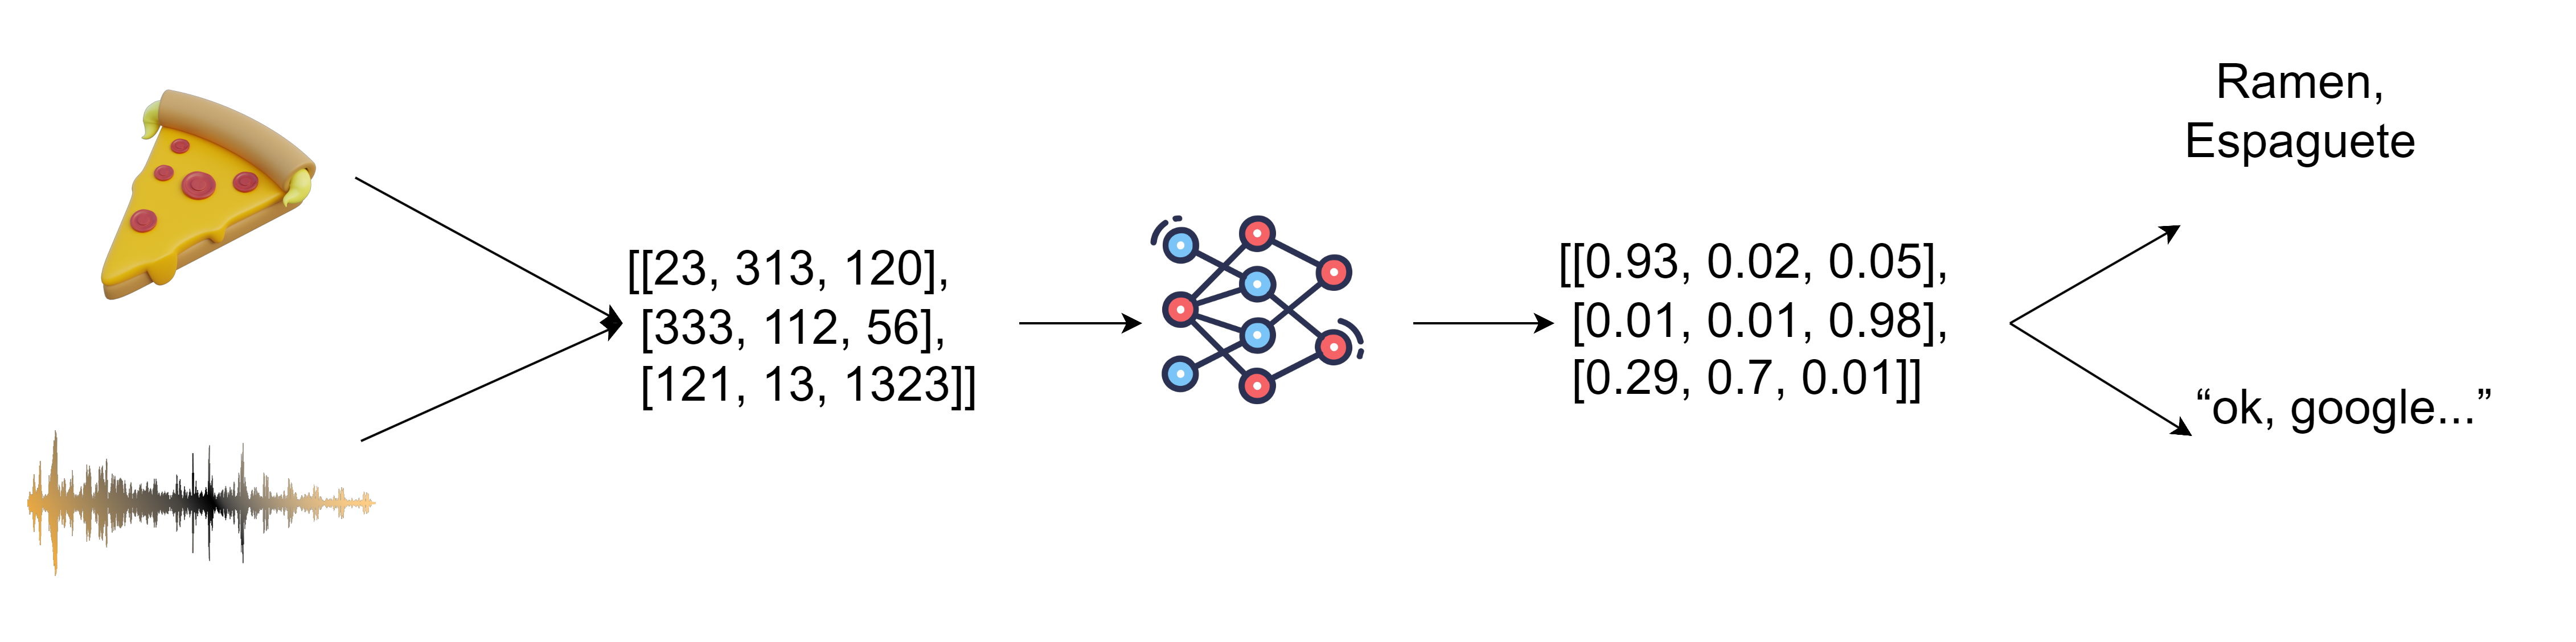
\includegraphics[width=1\linewidth]{figures/workflow_nn}
	\end{figure}
	
	\end{block}
\end{frame}

%==========================================================================================
\section{Pytorch Regressão Linear}

\begin{frame}
	\frametitle{Pytorch Regressão Linear}
	\begin{block}{Pytorch Regressão Linear}
		
		Se recordam da fórmula da função linear? 
		$$y = a + b*X$$
		
		Vamos ver isso diretamente no notebook enquanto acompanhamos os slides! \\
		Agora vamos avançar para a construção de um modelo que pode aprender a relação entre X (features) e y (labels).
	\end{block}
\begin{alertblock}{Nota}
	Vamos usar o notebook 08
\end{alertblock}
\end{frame}
%==========================================================================================

\begin{frame}
	\frametitle{Pytorch Regressão Linear}
	\begin{block}{Divida os dados em conjuntos de treinamento e teste}
		Temos alguns dados. 
		
		Mas antes de construirmos um modelo, precisamos dividi-lo. 
		
		Uma das etapas mais importantes em um projeto de aprendizado de máquina é criar um conjunto de treinamento e teste (e, quando necessário, um conjunto de validação). 
		
		Cada divisão do conjunto de dados serve a um propósito específico:
		\begin{table}[]
			\resizebox{\textwidth}{!}{%
				\begin{tabular}{|l|l|l|l|}
					\hline
					Divisão &
					Objetivo &
					Qtd. de dados &
					Frequência \\ \hline
					Treinamento &
					\begin{tabular}[c]{@{}l@{}}O modelo aprende com esses dados\\ (como os materiais do curso que você estuda durante o semestre).\end{tabular} &
					$\sim$60-80\% &
					Sempre \\ \hline
					Validação &
					\begin{tabular}[c]{@{}l@{}}O modelo é ajustado nesses dados\\ (como o exame simulado que você faz antes do exame final).\end{tabular} &
					$\sim$10-20\% &
					\begin{tabular}[c]{@{}l@{}}Muitas vezes\\ mas nem sempre\end{tabular} \\ \hline
					Teste &
					\begin{tabular}[c]{@{}l@{}}O modelo é avaliado com base nesses dados para testar o que aprendeu\\ (como o exame final que você faz no final do semestre)\end{tabular} &
					$\sim$10-20\% &
					Sempre \\ \hline
				\end{tabular}%
			}
		\end{table}
		Por enquanto, usaremos apenas um conjunto de treinamento e teste, o que significa que teremos um conjunto de dados para nosso modelo aprender e também ser avaliado.
	\end{block}
\end{frame}
%==========================================================================================
\begin{frame}
	\frametitle{Pytorch Regressão Linear}
	\begin{block}{Divida os dados em conjuntos de treinamento e teste}
		
		Podemos criá-los dividindo nossos tensores $X$ e $y$.
		
		\textbf{Observação:} Ao lidar com dados do mundo real, esta etapa normalmente é realizada logo no início de um projeto (o conjunto de teste sempre deve ser mantido separado de todos os outros dados). Queremos que nosso modelo aprenda com os dados de treinamento e depois os avalie com os dados de teste para obter uma indicação de quão bem ele \textbf{generaliza} para exemplos não vistos.
		
		O modelo que criamos vai tentar aprender a relação entre X\_train e y\_train e então avaliaremos o que ele aprende em X\_test e y\_test.
		
		Mas agora nossos dados são apenas números em uma página.
		
		Vamos criar uma função para visualizá-lo.
	\end{block}
\end{frame}
%==========================================================================================

\begin{frame}
	\frametitle{Pytorch Regressão Linear}
	\begin{block}{Vizualize, vizualize, vizualize!}
		Observação: agora é um bom momento para apresentar a você o lema do explorador de dados... "visualize, visualize, visualize!"
		
		Pense nisso sempre que estiver trabalhando com dados e transformando-os em números, se você pode visualizar algo, pode fazer maravilhas para a compreensão.
		
		As máquinas adoram números e nós, humanos, também gostamos de números, mas também gostamos de olhar para as coisas.
	\end{block}
\end{frame}
%==========================================================================================
\begin{frame}
	\frametitle{Pytorch Regressão Linear - Construção do Modelo}
	\begin{block}{Fundamentos da construção de modelos PyTorch}
		PyTorch tem quatro (mais ou menos) módulos essenciais que você pode usar para criar quase qualquer tipo de rede neural que você possa imaginar.
		
		Eles são torch.nn, torch.optim, torch.utils.data.Dataset e torch.utils.data.DataLoader. Por enquanto, vamos nos concentrar nos dois primeiros e chegar aos outros dois mais tarde (embora você possa adivinhar o que eles fazem).
		
		% Please add the following required packages to your document preamble:
		% \usepackage{graphicx}
		\begin{table}[]
			\resizebox{\textwidth}{!}{%
				\begin{tabular}{|l|l|}
					\hline
					\textbf{Módulo PyTorch} &
					\textbf{Objetivo} \\ \hline
					torch.nn &
					\begin{tabular}[c]{@{}l@{}}Contém todos os blocos de construção para gráficos computacionais\\ (essencialmente uma série de cálculos executados de uma maneira particular).\end{tabular} \\ \hline
					torch.nn.Parameter &
					\begin{tabular}[c]{@{}l@{}}Armazena tensores que podem ser usados com nn.Module. Se os gradientes requires\_grad=True\\ (usados para atualizar os parâmetros do modelo por meio de gradient descent) forem calculados automaticamente,\\ isso é muitas vezes referido como "autogrado".\end{tabular} \\ \hline
					torch.nn.Module &
					\begin{tabular}[c]{@{}l@{}}A classe base para todos os módulos de rede neural, todos os blocos de construção para redes neurais são subclasses.\\ Se você estiver construindo uma rede neural no PyTorch, seus modelos devem subclassificar nn.Module.\\ Requer que um método forward() seja implementado.\end{tabular} \\ \hline
					torch.optim &
					\begin{tabular}[c]{@{}l@{}}Contém vários algoritmos de otimização (estes dizem aos parâmetros do modelo armazenados em\\ nn.Parameter como alterar melhor para melhorar a descida do gradiente e, por sua vez, reduzir a perda).\end{tabular} \\ \hline
					def forward() &
					\begin{tabular}[c]{@{}l@{}}Todas as subclasses nn.Module requerem um método forward(), que define a computação que ocorrerá\\ nos dados passados para o nn.Module específico (por exemplo, a fórmula de regressão linear acima).\end{tabular} \\ \hline
				\end{tabular}%
			}
		\end{table}
	\end{block}
\end{frame}
%==========================================================================================
\begin{frame}
	\frametitle{Pytorch Regressão Linear - Construção do Modelo}
	\begin{block}{Fundamentos da construção de modelos PyTorch}
		\begin{figure}
			\centering
			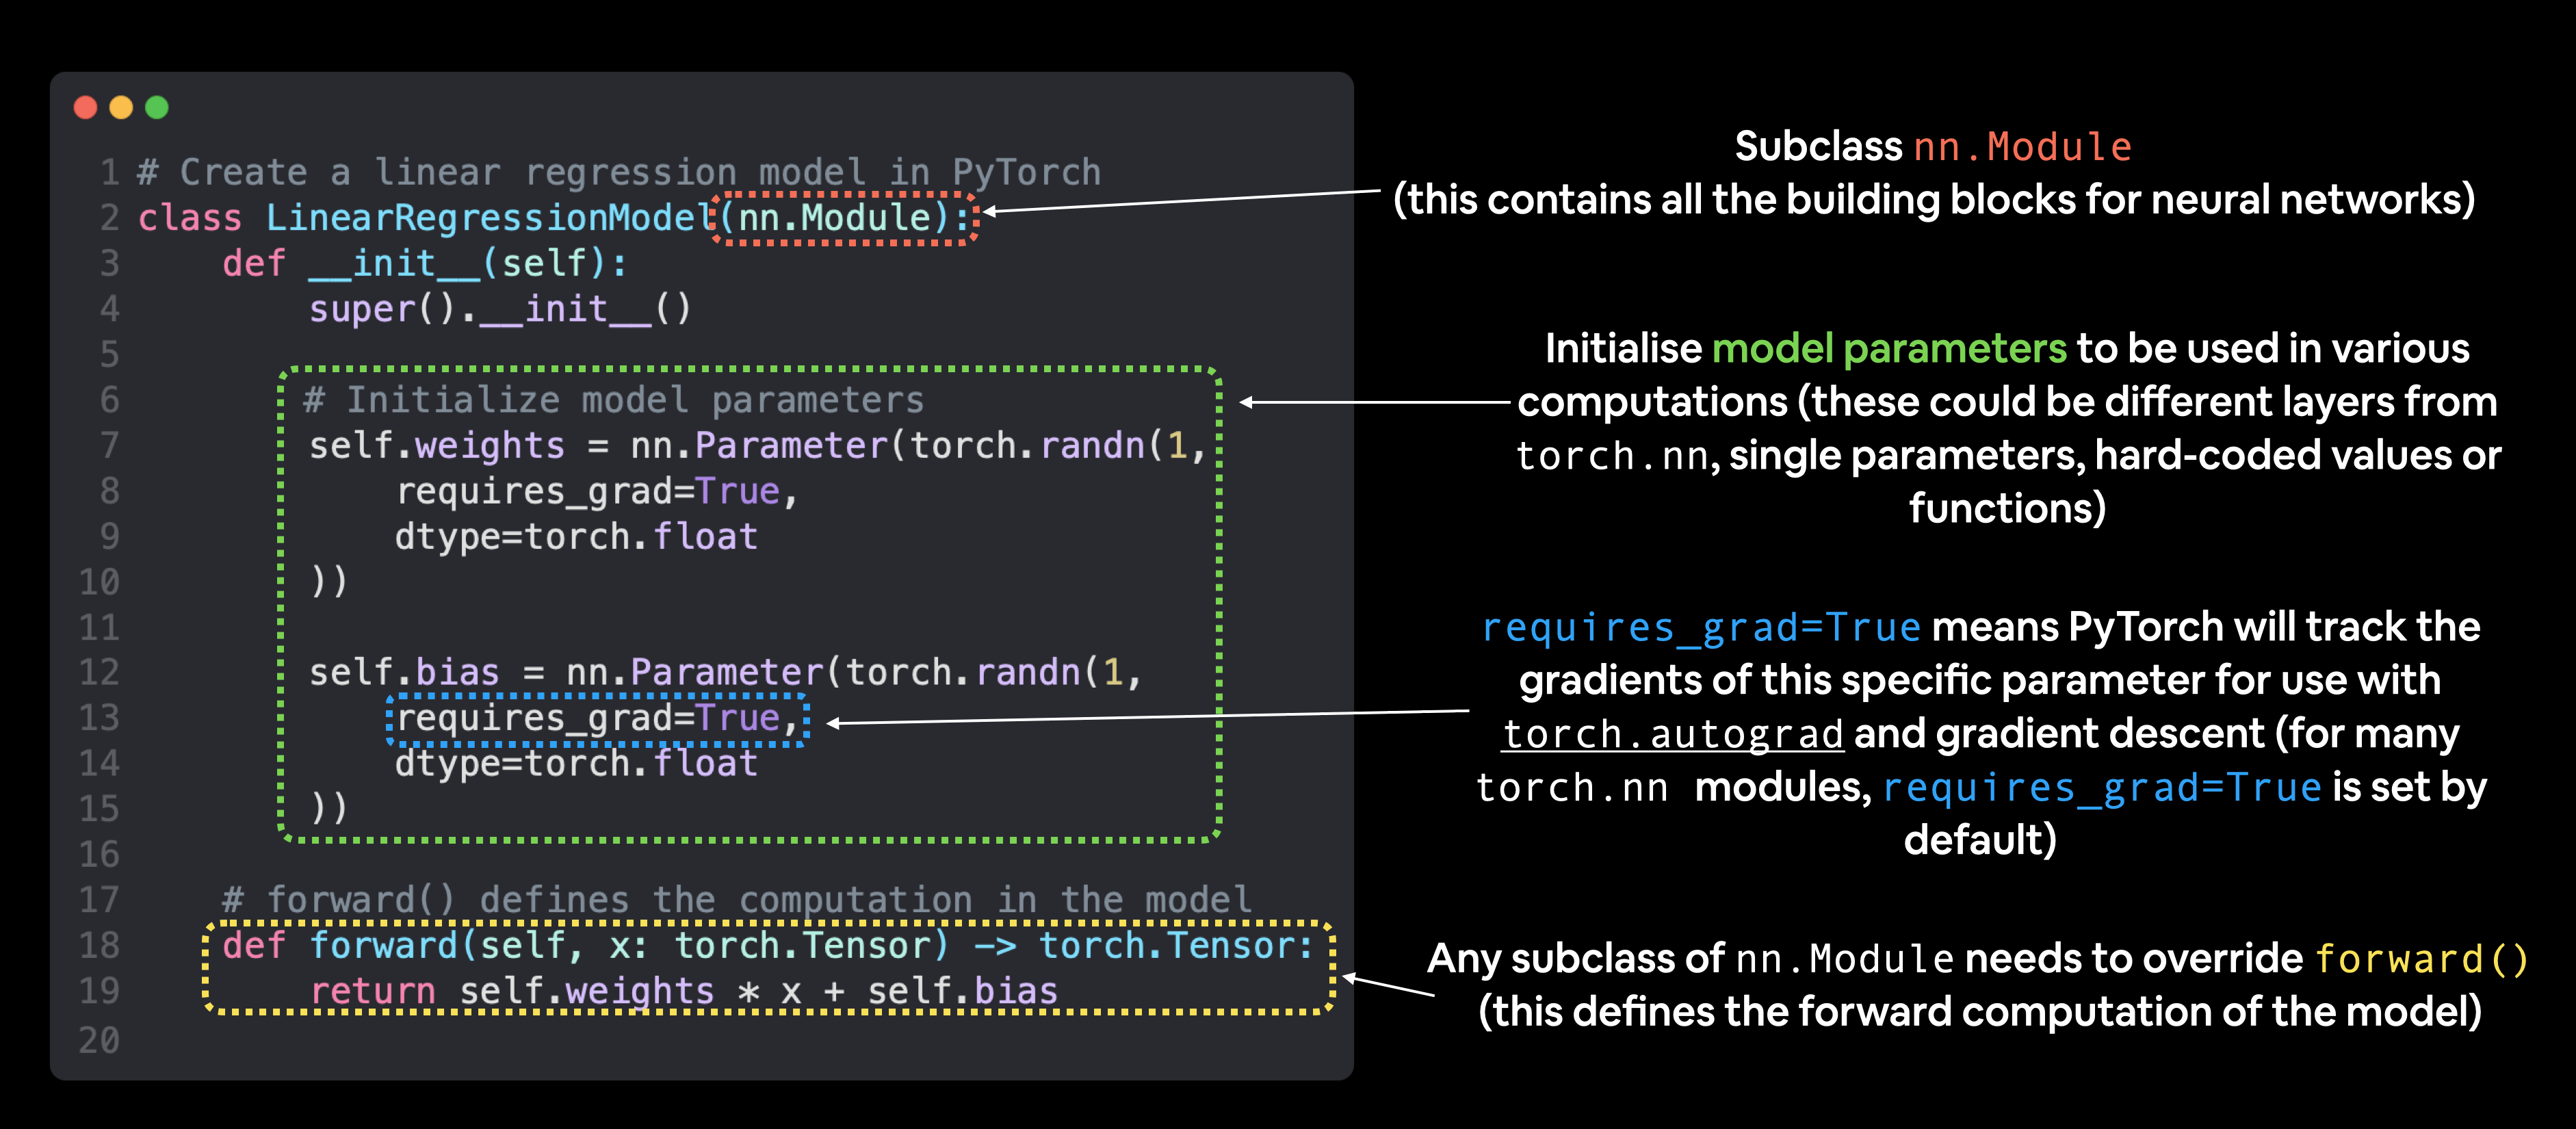
\includegraphics[width=1\linewidth]{figures/basic_torch_implmentation}
		\end{figure}
		
	\end{block}
\end{frame}
%==========================================================================================
\begin{frame}
	\frametitle{Pytorch Regressão Linear - Fazendo predições}
	\begin{block}{Fazendo predições sem treinar o modelo}
		\begin{figure}
			\centering
			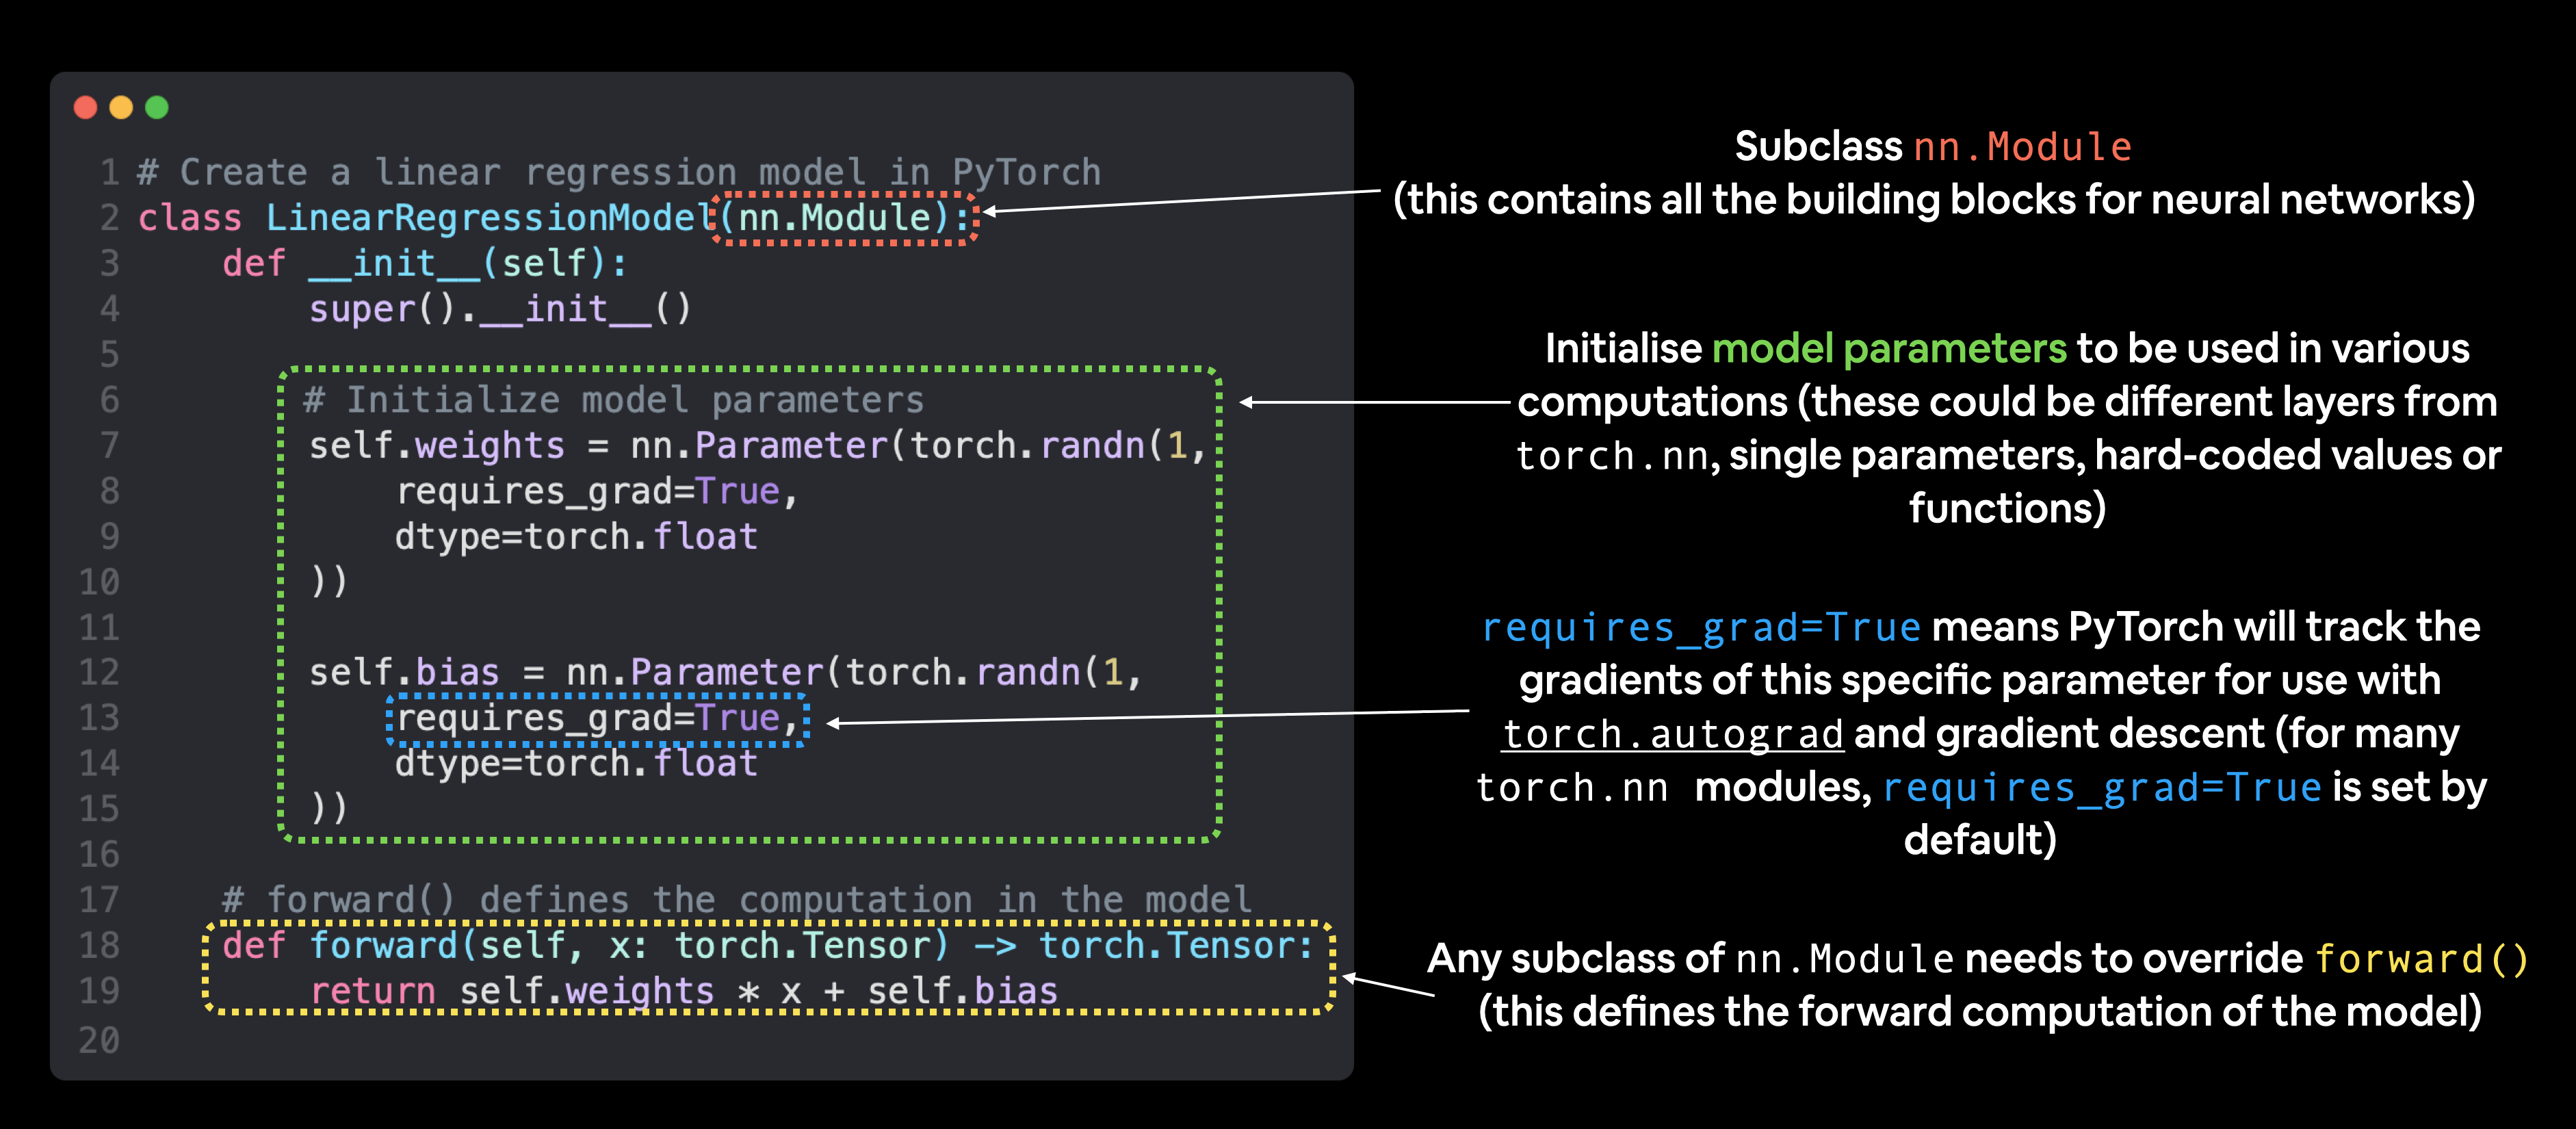
\includegraphics[width=1\linewidth]{figures/basic_torch_implmentation}
		\end{figure}
		
	\end{block}
\end{frame}
%==========================================================================================
\begin{frame}
	\frametitle{Pytorch Regressão Linear - Treinando o Modelo}
	\begin{block}{Treinando o modelo}
		\begin{itemize}
			\item Selecione a função de perda:
			\begin{itemize}
				\item Mean absolute error (MAE) for regression problems (torch.nn.L1Loss())
				\item Binary cross entropy for binary classification problems (torch.nn.BCELoss()).
			\end{itemize}
			\item Selecione seu otimizador:
				\begin{itemize}
					\item Stochastic gradient descent (torch.optim.SGD()).
					\item Adam optimizer (torch.optim.Adam()).
				\end{itemize}
			\item Crie seu loop de teinamento!
		\end{itemize}
		
	\end{block}
\end{frame}
%==========================================================================================
\begin{frame}
	\frametitle{Pytorch Regressão Linear - Treinando o Modelo}
	\begin{block}{Criando o loop de treinamento do modelo para o \textbf{Treinamento}}
		\begin{itemize}
			\item[1] Forward pass $model(x_train)$ 
			\item[2] Calcule a perda $loss = loss_fn(y_pred, y_train)$
			\item[3] Gradientes zero $optimizer.zero_grad()$
			\item[4] Executar retropropagação na perda $loss.backward()$
			\item[5] Atualize o otimizador (descida de gradiente) $optimizer.step()$
		\end{itemize}
		\begin{figure}
			\centering
			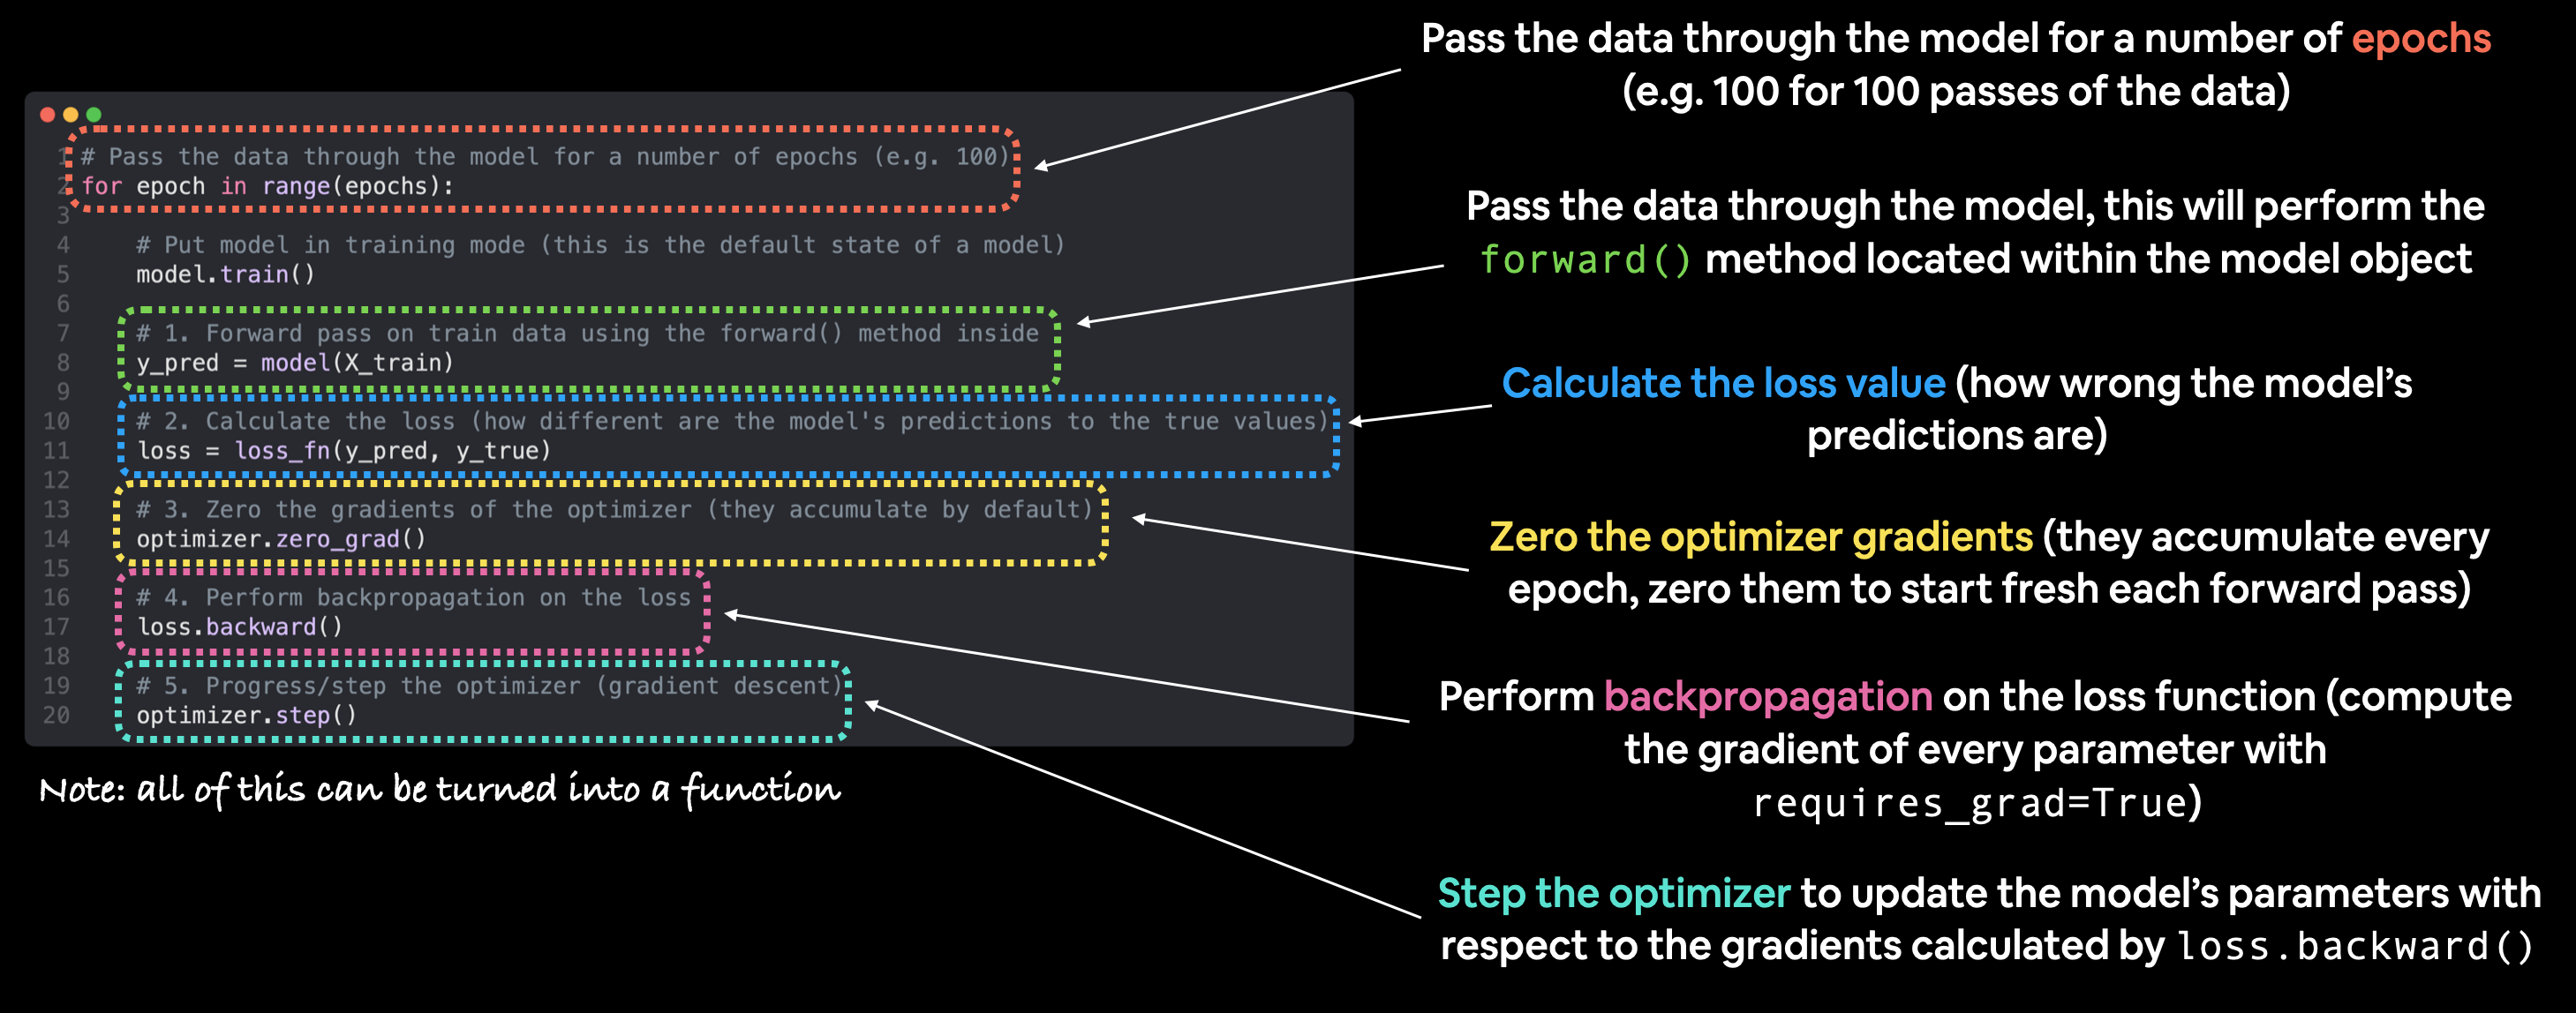
\includegraphics[width=0.7\linewidth]{figures/steps_train_torch}
		\end{figure}
		
	\end{block}
\end{frame}
%==========================================================================================

\begin{frame}
	\frametitle{Pytorch Regressão Linear - Treinando o Modelo}
	\begin{block}{Criando o loop de treinamento do modelo para o \textbf{Teste}}
		\begin{itemize}
			\item[1] Forward pass $model(x_train)$ 
			\item[2] Calcule a perda $loss = loss_fn(y_pred, y_train)$
			\item[3] Calulate evaluation metrics (optional) $Custom functions$
		\end{itemize}
		\begin{figure}
			\centering
			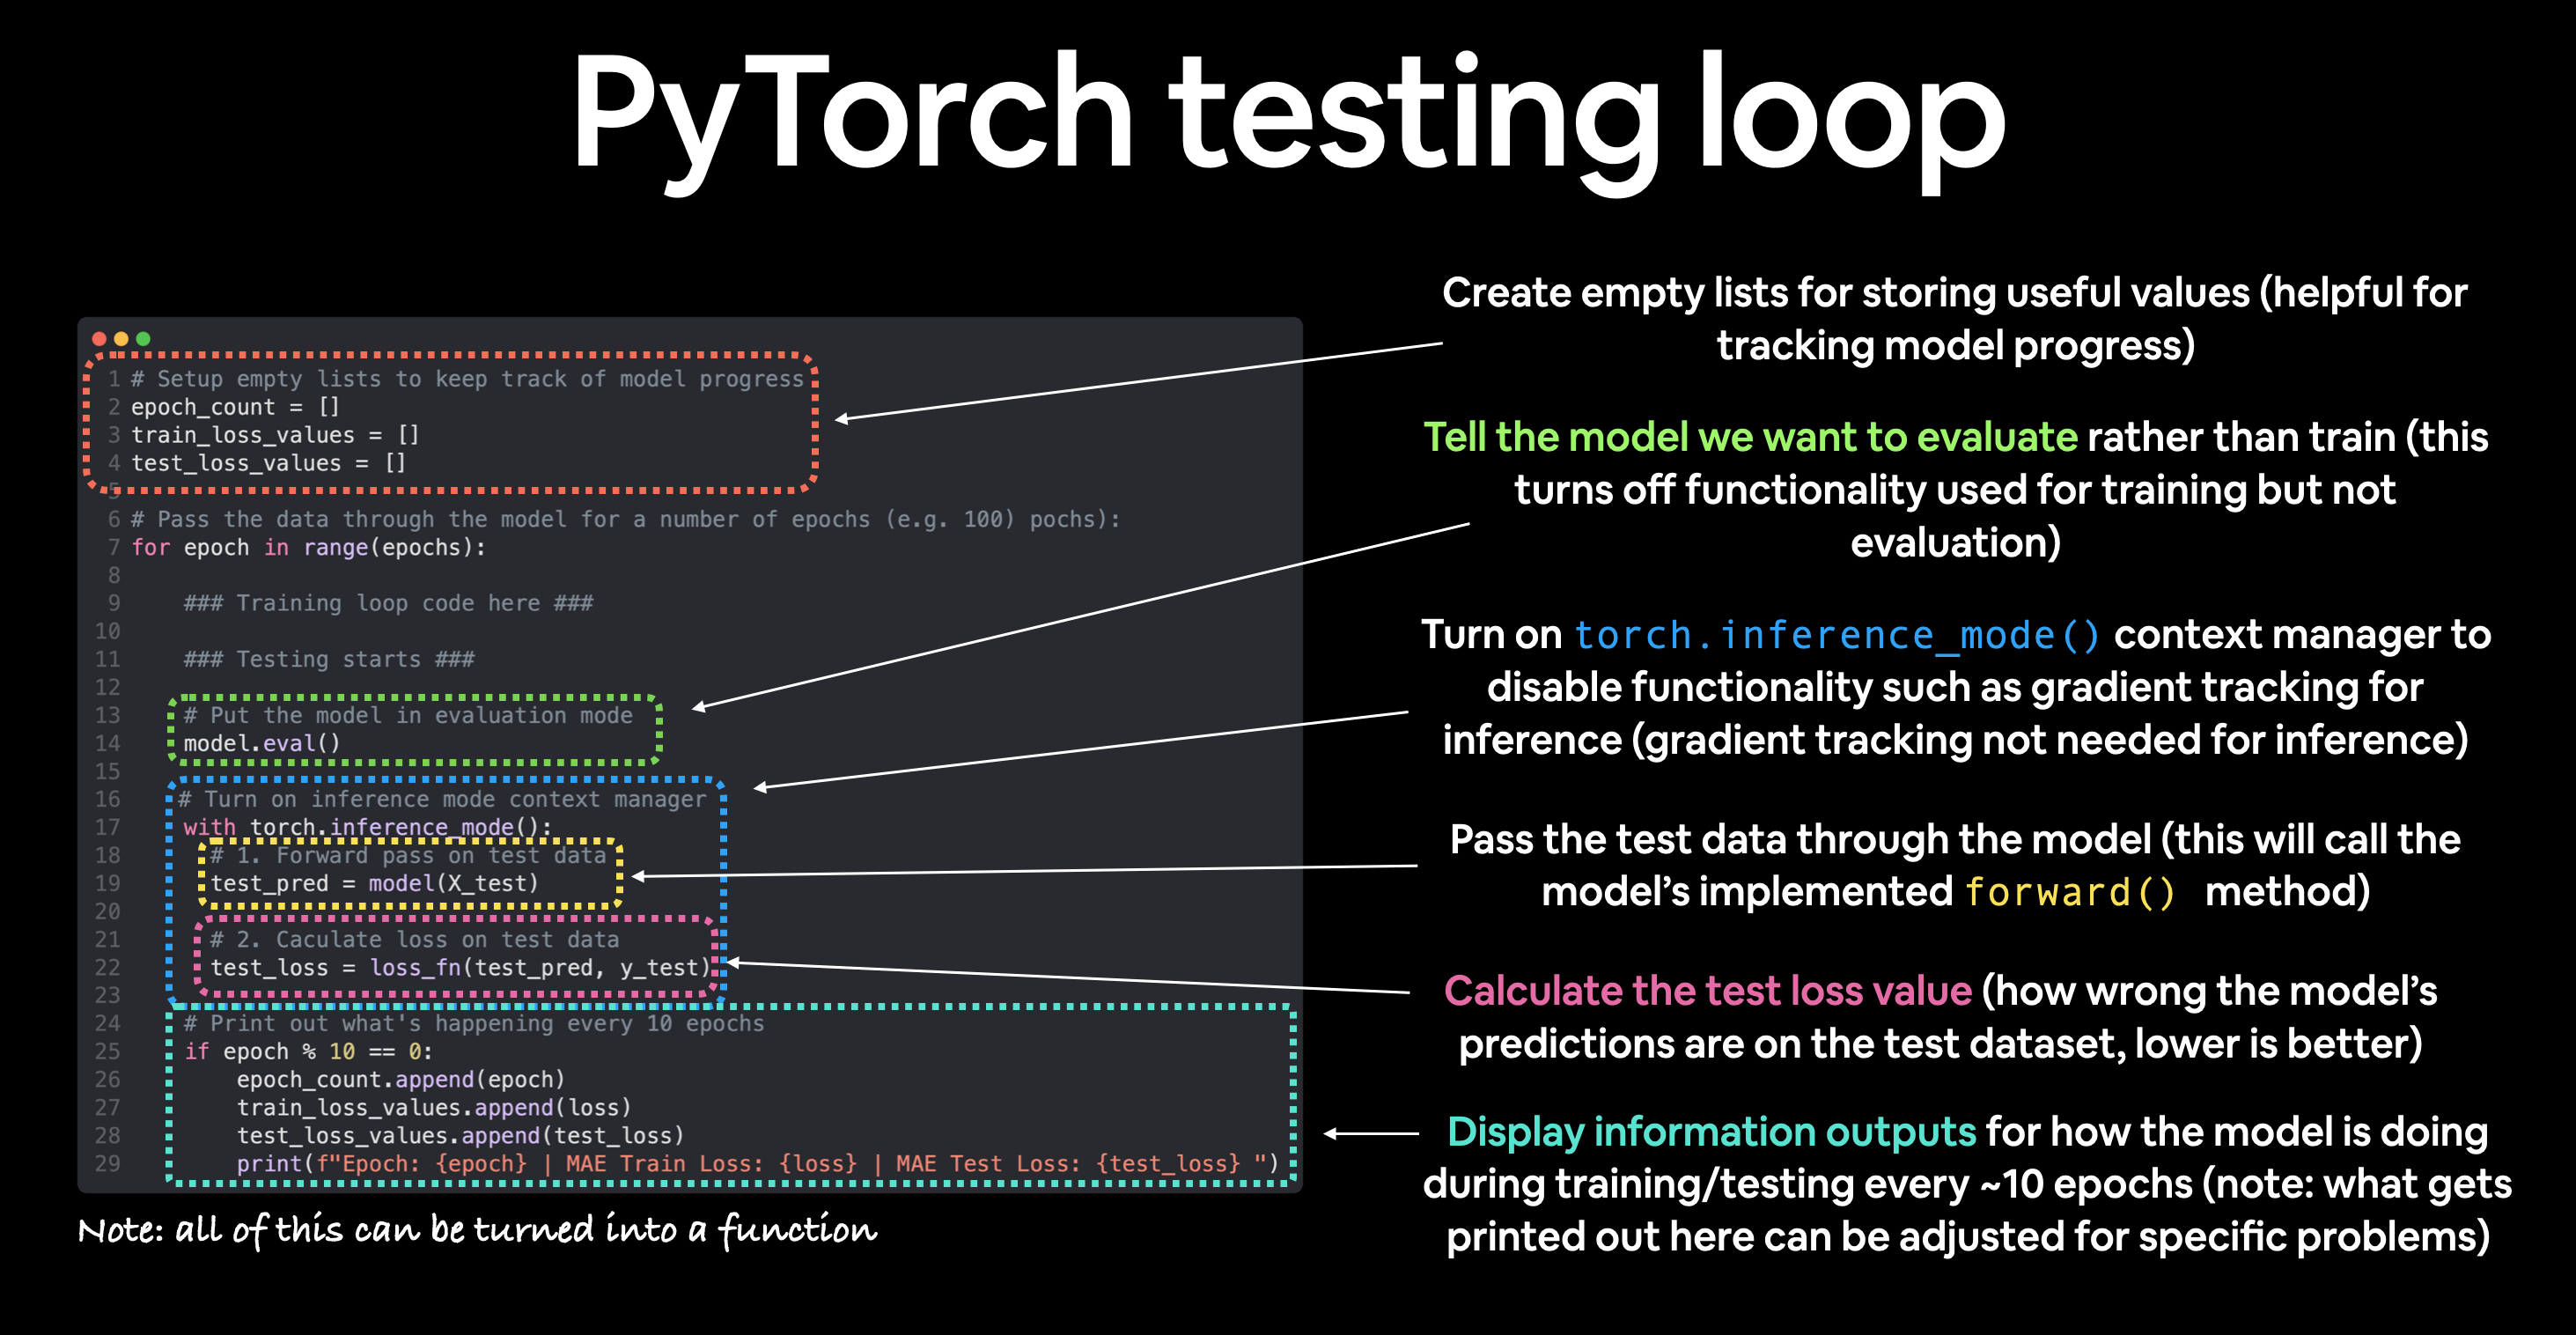
\includegraphics[width=0.7\linewidth]{figures/steps_test_torch}
		\end{figure}
		
	\end{block}
\end{frame}
%==========================================================================================
\begin{frame}
	\frametitle{Pytorch Regressão Linear - Fazendo predições com o Modelo Treinado}
	\begin{block}{Fazendo predições com o Modelo Treinado}
		\begin{itemize}
			\item[1] Mude para o modo de avaliação $model_0.eval()$
			\item[2] Faça as pervisões $y_preds = model_0(X_test)$
		\end{itemize}
	
	\end{block}
\end{frame}
%==========================================================================================
\begin{frame}
	\frametitle{Pytorch Regressão Linear - Salve o Modelo Treinado}
	\begin{block}{Salve o Modelo Treinado}
		Se você treinou um modelo PyTorch, é provável que queira salvá-lo e exportá-lo para algum lugar.
		
		Por exemplo, você pode treiná-lo no Google Colab ou em sua máquina local com uma GPU, mas agora gostaria de exportá-lo para algum tipo de aplicativo onde outras pessoas possam usá-lo.
		
		Ou talvez você queira salvar seu progresso em um modelo e voltar e carregá-lo mais tarde.
		\begin{itemize}
			\item[1] Salve o modelo treinado
			\item[2] Carregue o modelo salvo
			\item[3] Faça predições com o modelo carregado
		\end{itemize}
		
	\end{block}
\end{frame}
%==========================================================================================
\begin{frame}
	\frametitle{Pytorch Regressão Linear - Vamos criar o mesmo modelo de forma mais simples}
	\begin{block}{Novo Modelo}
		\begin{itemize}
			\item[1] Crie os dados para o modelo
			\item[2] Construa o modelo
			\item[3] Selecione a função de perda
			\item[4] Selecione o otimizador
			\item[5] Crie o loop de treinamento
			\item[6] Faça predições
			\item[7] Salve o modelo treinado
			\item[8] Carregue o modelo salvo
			\item[9] Faça predições com o modelo carregado
		\end{itemize}
		
	\end{block}
\end{frame}

%==========================================================================================
%==========================================================================================
\section{PyTorch Neural Network Classification}

\begin{frame}
	\frametitle{PyTorch Neural Network Classification}
	\begin{block}{PyTorch Neural Network Classification}
		\textbf{Binary classification:} Target can be one of two options, e.g. yes or no. Predict whether or not someone has heart disease based on their health parameters. 
		
		\textbf{Multi-class classification:} Target can be one of more than two options. Decide whether a photo of is of food, a person or a dog.
		
		\textbf{Multi-label classification:} Target can be assigned more than one option. Predict what categories should be assigned to a Wikipedia article (e.g. mathematics, science e philosohpy).
	\end{block}
\end{frame}
%==========================================================================================
\begin{frame}
	\frametitle{PyTorch Neural Network Classification}
	\begin{block}{PyTorch Neural Network Classification}
		O que vamos ver:
		\begin{itemize}
			\item Arquitetura de uma rede neural de classificação
			\item Preparando os dados de classificação binária
			\item Construindo um modelo de classificação PyTorch
			\item Ajustando o modelo aos dados (treinamento)
			\item Fazendo previsões e avaliando um modelo (inferência)
			\item Melhorando um modelo (de uma perspectiva de modelo)
			\item Não linearidade
			\item Replicando funções não lineares
			\item Juntando tudo com a classificação multiclasse
		\end{itemize}
	\end{block}
\end{frame}
%==========================================================================================
\begin{frame}
	\frametitle{PyTorch Neural Network Classification}
	\begin{block}{Arquitetura de uma rede neural de classificação}
		\begin{itemize}
			\item\textbf{Input layer shape (in\_features):} Same as number of features (e.g. 5 for age, sex, height, weight, smoking status in heart disease prediction)
			\item \textbf{Hidden layer(s):} Problem specific, minimum = 1, maximum = unlimited
			\item \textbf{Neurons per hidden layer:} Problem specific, generally 10 to 512
			\item \textbf{Output layer shape (out\_features):} 1 (one class or the other)
			\item \textbf{Hidden layer activation:} Usually ReLU (rectified linear unit) but can be many others
			\item \textbf{Output activation:} Sigmoid (torch.sigmoid in PyTorch)
			\item \textbf{Loss function:} Binary crossentropy (torch.nn.BCELoss in PyTorch)
			\item \textbf{Optimizer:} SGD (stochastic gradient descent), Adam (see torch.optim for more options)
		\end{itemize}
	\end{block}
\end{frame}
%==========================================================================================
\begin{frame}
	\frametitle{PyTorch Neural Network Classification}
	\begin{block}{Arquitetura de uma rede neural de classificação}
	Vamos ver isso no notebook, com o problema dos círculos!
	\begin{figure}
		\centering
		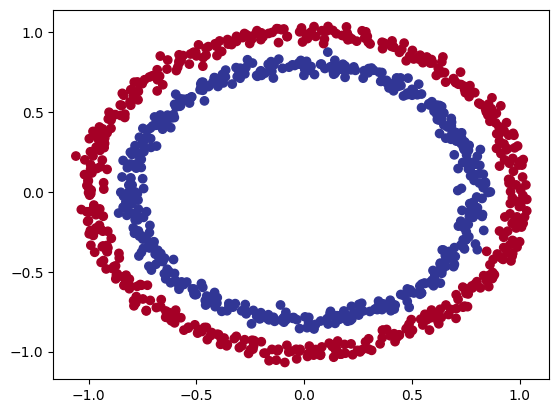
\includegraphics[width=0.4\linewidth]{figures/make_circle}
	\end{figure}
	Vamos ver este exemplo no TensorFlow Playground website \\
	\href{https://playground.tensorflow.org/}{\beamergotobutton{TensorFlow Playground website}} \\
	Vamos replicar este exemplo! \\
	Vamos descobrir como poderíamos construir uma rede neural PyTorch para classificar pontos em vermelho (0) ou azul (1).
	\end{block}
\end{frame}
%==========================================================================================
\begin{frame}
	\frametitle{PyTorch Neural Network Classification}
	\begin{block}{Arquitetura de uma rede neural de classificação}
		Os passos que vamos fazer:
		\begin{itemize}
			\item Vizualizar o shape dos dados $X.shape, y.shape$
			\item Transformar os dados em tensores: $torch.from\_numpy(X).type(torch.float)$
			\item Dividir em Train e Test: $train\_test\_split$
			\item Construir o modelo
			\item Fazer predições (sem treinamento)
			\item Escolher função de custo e Otimizador (no próximo slide)
			\item Desenvolver métrica de avaliação: $accuracy\_fn$
			\item Acessar: (https://datascience.stackexchange.com/a/31045)
		\end{itemize}
	\end{block}
\end{frame}
%==========================================================================================
\begin{frame}
	\frametitle{PyTorch Neural Network Classification}
	\begin{block}{Arquitetura de uma rede neural de classificação}
		Os passos que vamos fazer:
		% Please add the following required packages to your document preamble:
		% \usepackage{graphicx}
		\begin{table}[]
			\resizebox{\textwidth}{!}{%
				\begin{tabular}{|l|l|l|}
					\hline
					\textbf{Loss function/Optimizer}     & \textbf{Problem type}                    & \textbf{PyTorch Code}     \\ \hline
					Stochastic Gradient Descent (SGD) optimizer &
					Classification, regression, many others. &
					torch.optim.SGD() \\ \hline
					Adam Optimizer                       & Classification, regression, many others. & torch.optim.Adam()        \\ \hline
					Binary cross entropy loss &
					Binary classification &
					\begin{tabular}[c]{@{}l@{}}torch.nn.BCELossWithLogits\\ or torch.nn.BCELoss\end{tabular} \\ \hline
					Cross entropy loss                   & Multi-class classification               & torch.nn.CrossEntropyLoss \\ \hline
					Mean absolute error (MAE) or L1 Loss & Regression                               & torch.nn.L1Loss           \\ \hline
					Mean squared error (MSE) or L2 Loss  & Regression                               & torch.nn.MSELoss          \\ \hline
				\end{tabular}%
			}
		\end{table}
	\end{block}
\end{frame}
%==========================================================================================
\begin{frame}
	\frametitle{PyTorch Neural Network Classification}
	\begin{block}{Arquitetura de uma rede neural de classificação}
		Os passos que vamos fazer:
		\begin{itemize}
			\item Construir loop de treinamento
			\item Treinar o modelo 
			\item Analisar resultados: Se o modelo predizer todos os dados com a mesma classe a acurácia será 50\%. O que está acontecendo com o nosso modelo?
			\item Visualizar os nossos resultados: O lema do explorador de dados!
			\item Separação dos dados linearmente?
		\end{itemize}
	Vamos ver alguns ajustes que podemos fazer a seguir!
	\end{block}
\end{frame}
%==========================================================================================
\begin{frame}
	\frametitle{PyTorch Neural Network Classification}
	\begin{block}{Arquitetura de uma rede neural de classificação}
		A seguir estão algumas dicas para livrar seu modelo do problema de underfitting:
		\begin{itemize}
			\item Adicionar mais camadas
			\item Adicionar mais neurônios 
			\item Treinar por mais épocas
			\item Mudar as camadas de ativação
			\item Alterar o Learning Rate
			\item Alterar a função de perda
			\item Usar Transfering Learning
		\end{itemize}
	Esse tipo de alteração se referem as mudanças de hiperparâmetros! \\
	Vamos continuar tentando melhorar este modelo...
	\end{block}
\end{frame}
%==========================================================================================
\begin{frame}
	\frametitle{PyTorch Neural Network Classification}
	\begin{block}{Arquitetura de uma rede neural de classificação}
		\begin{itemize}
			\item Adicionar mais camadas
			\item Visualizar e analisar o resultado!
			\item Vamos construir um modelo não-linear!
			\item Vamos treinar o modelo
			\item Vamos analisar o desempenho do modelo
		\end{itemize}
	\end{block}
\end{frame}
%==========================================================================================
\begin{frame}
	\frametitle{PyTorch Neural Network Classification}
	\begin{block}{Arquitetura de uma rede neural de classificação}
		Vamos construir um modelo de classificação multi-classe
		\begin{itemize}
			\item Criar os dados
			\item Criar modelo - Selecionar Loss Function e Optimizer e Testá-lo
			\item Vamos treinar o modelo, testar e analisar o desempenho do modelo
		\end{itemize}
		\begin{figure}
			\centering
			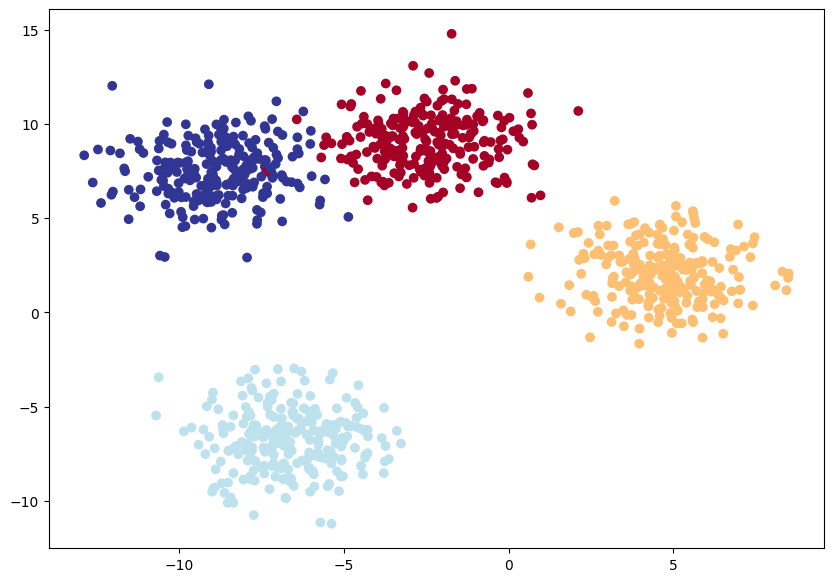
\includegraphics[width=0.3\linewidth]{figures/multiclass_example}
		\end{figure}
	\end{block}
\begin{alertblock}{Pergunta}
	Precisamos de não-linearidade para classificar estes dados?
\end{alertblock}
\end{frame}
%==========================================================================================
\begin{frame}
	\frametitle{PyTorch Neural Network Classification}
	\begin{block}{Métricas de avaliação do modelo}
	% Please add the following required packages to your document preamble:
	% \usepackage{graphicx}
	\begin{table}[]
		\resizebox{\textwidth}{!}{%
			\begin{tabular}{|l|l|l|}
				\hline
				\textbf{Metric} &
				\textbf{Defintion} &
				\textbf{PyTorch Code} \\ \hline
				Accuracy &
				\begin{tabular}[c]{@{}l@{}}Out of 100 predictions, how many does your model get correct?\\ E.g. 95\% accuracy means it gets 95/100 predictions correct.\end{tabular} &
				\begin{tabular}[c]{@{}l@{}}torchmetrics.Accuracy()\\ sklearn.metrics.accuracy\_score()\end{tabular} \\ \hline
				Precision &
				\begin{tabular}[c]{@{}l@{}}Proportion of true positives over total number of samples.\\ Higher precision leads to less false positives (model predicts 1 when it should've been 0).\end{tabular} &
				\begin{tabular}[c]{@{}l@{}}torchmetrics.Precision()\\ sklearn.metrics.precision\_score()\end{tabular} \\ \hline
				Recall &
				\begin{tabular}[c]{@{}l@{}}Proportion of true positives over total number of true positives and false negatives\\ (model predicts 0 when it should've been 1). Higher recall leads to less false negatives.\end{tabular} &
				\begin{tabular}[c]{@{}l@{}}torchmetrics.Recall()\\ sklearn.metrics.recall\_score()\end{tabular} \\ \hline
				F1-score &
				Combines precision and recall into one metric. 1 is best, 0 is worst. &
				\begin{tabular}[c]{@{}l@{}}torchmetrics.F1Score()\\ sklearn.metrics.f1\_score()\end{tabular} \\ \hline
				Confusion matrix &
				\begin{tabular}[c]{@{}l@{}}Compares the predicted values with the true values in a tabular way, if 100\% correct,\\ all values in the matrix will be top left to bottom right (diagnol line).\end{tabular} &
				\begin{tabular}[c]{@{}l@{}}torchmetrics.ConfusionMatrix\\ sklearn.metrics.plot\_confusion\_matrix()\end{tabular} \\ \hline
				Classification report &
				Collection of some of the main classification metrics such as precision, recall and f1-score. &
				sklearn.metrics.classification\_report() \\ \hline
			\end{tabular}%
		}
	\end{table}
	\end{block}
\end{frame}
%==========================================================================================

\section{PyTorch Computer Vision}


%==========================================================================================
\begin{frame}
	\frametitle{PyTorch Computer Vision}
	\begin{block}{Computer Vision}
		Vamos utilizar o notebook 09
			\begin{itemize}
			\item Arte de ensinar um computador a ver
			\item Modelo para classificar se uma foto é de um gato ou de um cachorro (classificação binária)
			\item Ou se a foto é de um gato, cachorro ou galinha (classificação multiclasse)
			\item Ou identificar onde um carro aparece em um quadro de vídeo (detecção de objeto)
			\item Ou descobrir onde diferentes objetos em uma imagem podem ser separados (segmentação panóptica)
			\item Usado no seu celular, câmera, indústria, medicina, etc.
		\end{itemize}
	\end{block}
\end{frame}

%==========================================================================================
\begin{frame}
	\frametitle{PyTorch Computer Vision}
	\begin{figure}
		\centering
		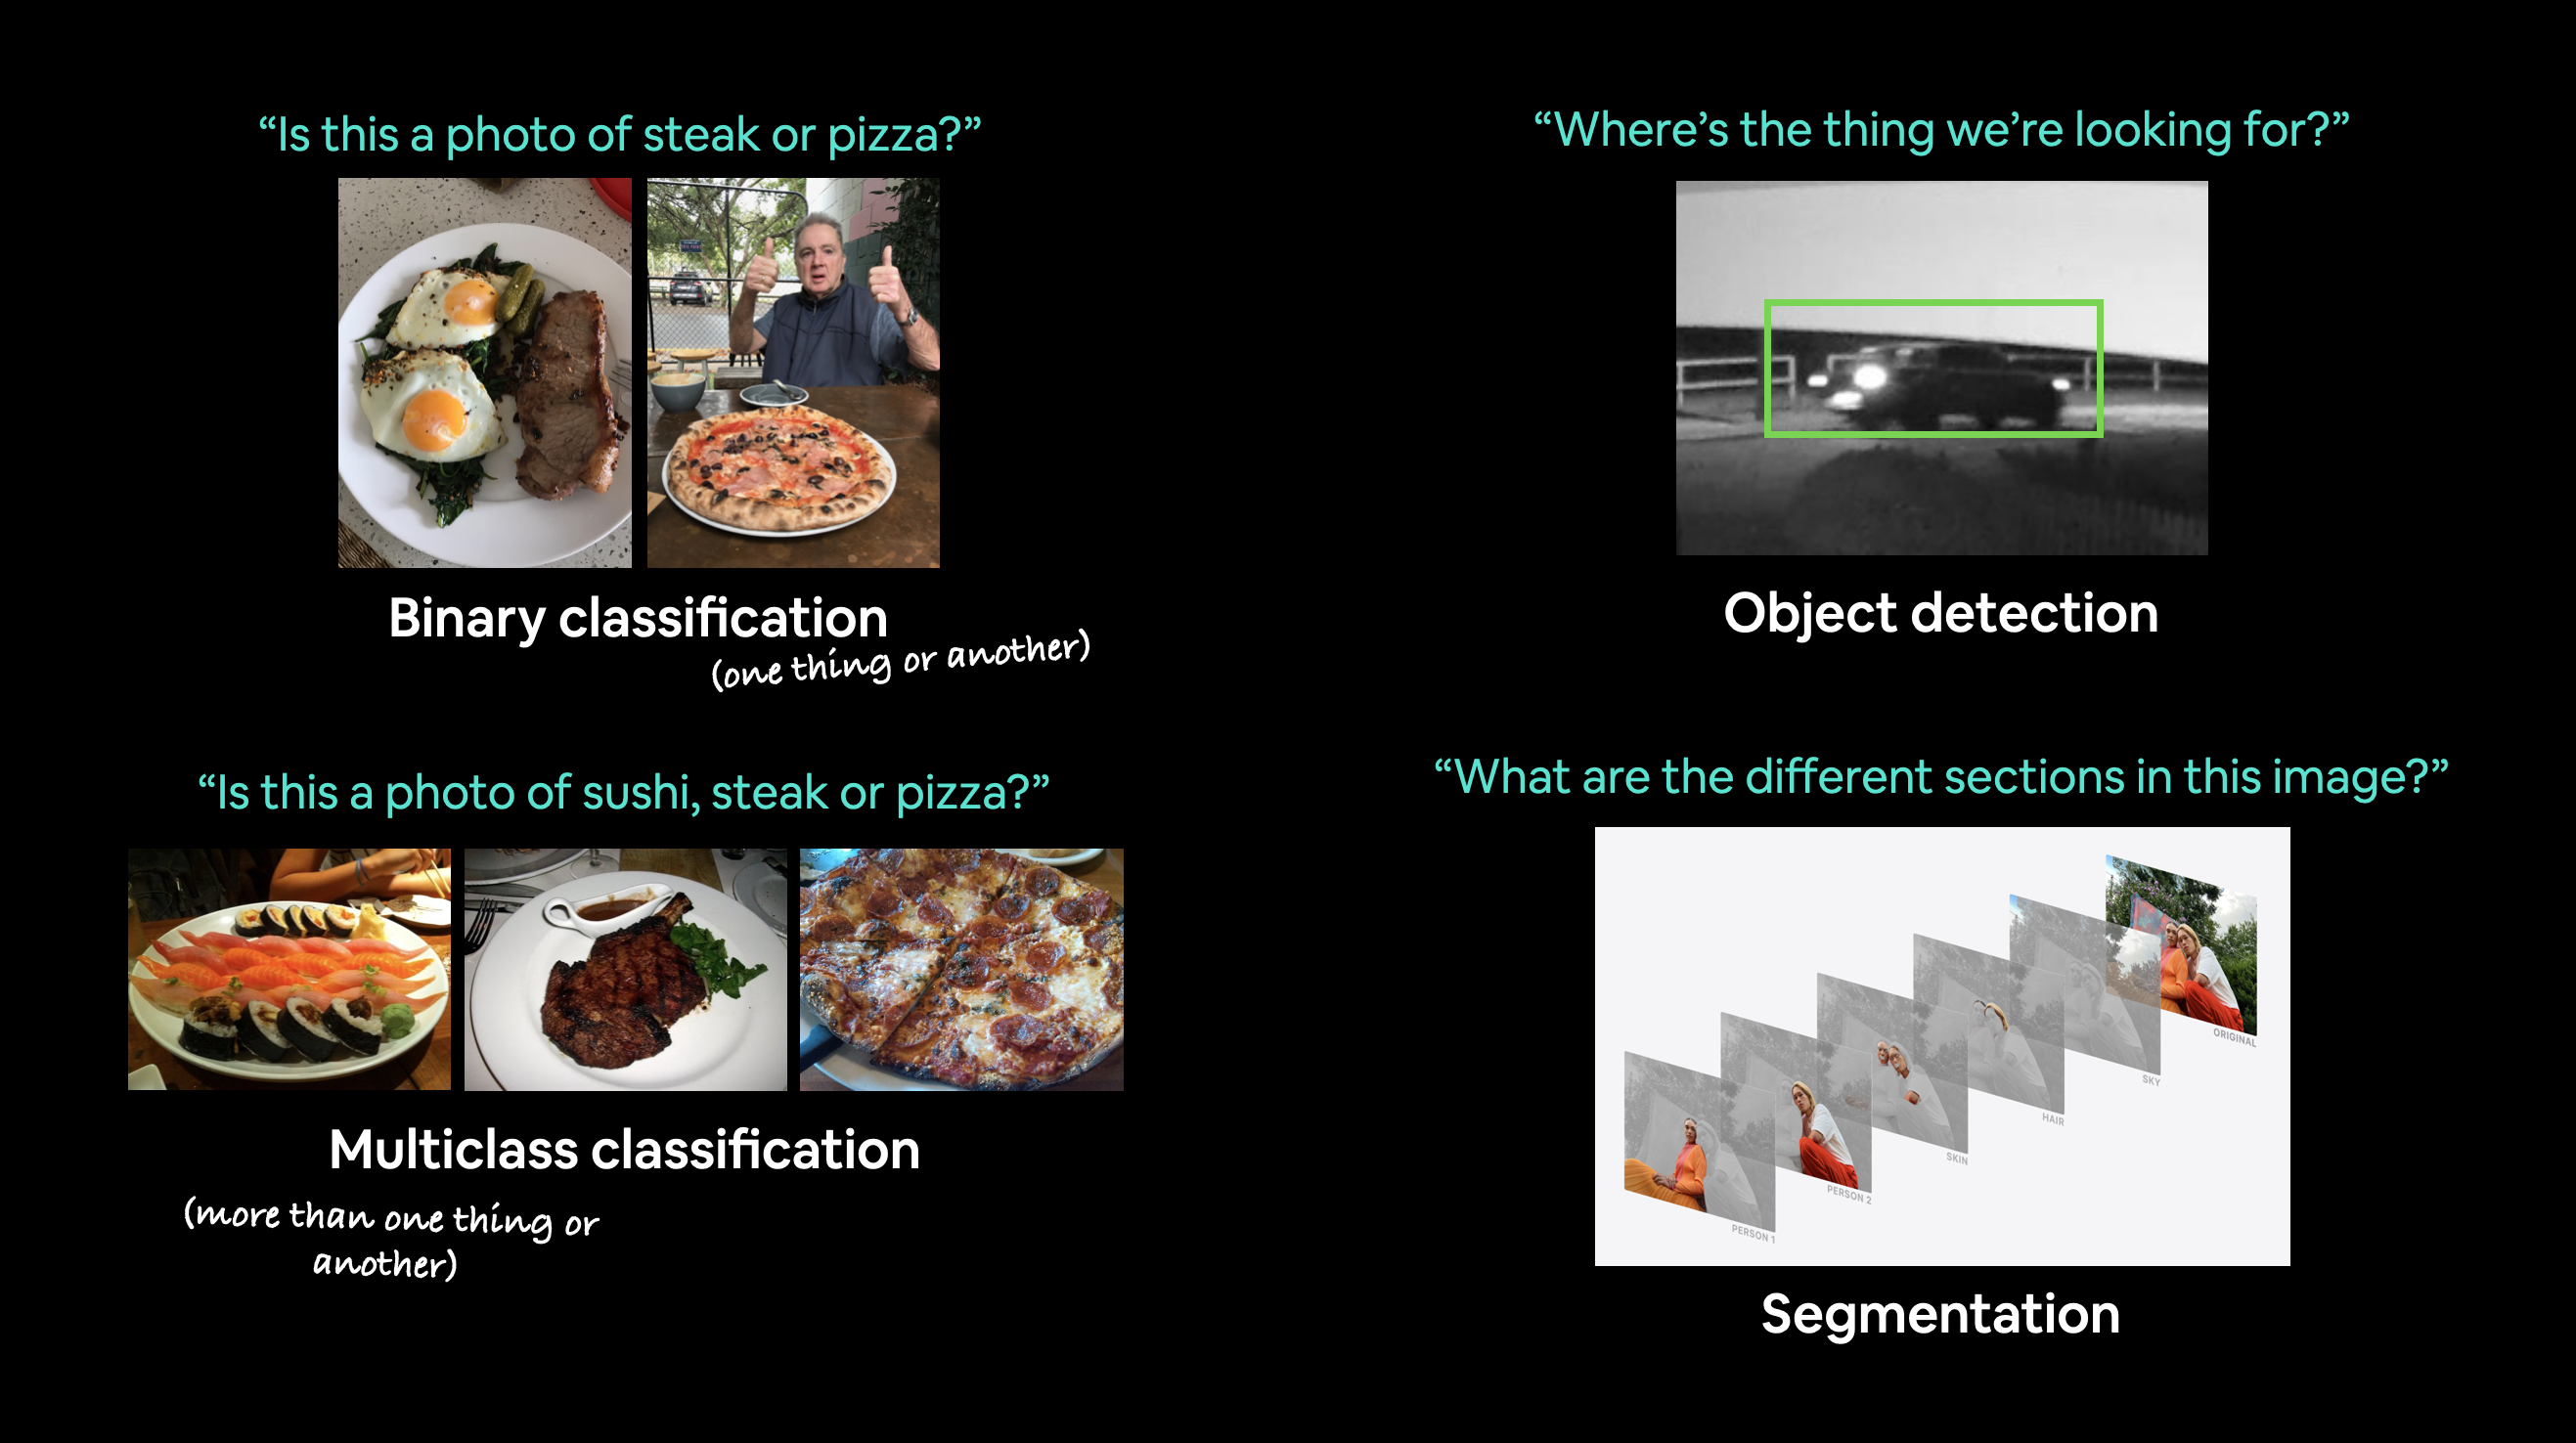
\includegraphics[width=1\linewidth]{figures/vision_comp}
	\end{figure}
	
\end{frame}
%==========================================================================================
\begin{frame}
	\frametitle{PyTorch Computer Vision}
	\begin{block}{Computer Vision - O que vamos fazer}
		\begin{itemize}
			\item Adquirindo o Dataset Fashion:
			\begin{itemize}
				\item Escala de cinza
				\item 10 tipos de roupas
			\end{itemize}
			\item Verificar a primeira amostra de dados de treinamento
			\item Vizualizar o Input e Output dos dados:
			\begin{itemize}
				\item Ordem dos dados no tensor: CHW (color channels first) or HWC (color channels last)
				\item NCHW - Número de imagens, Ex: batch\_size=32 - [32, 1, 28, 28]
			\end{itemize}
			\item Visualizar total de imagens de treinamento (60000) e teste (10000)
			\item Visualizar as 10 classes
			\item Visualizar uma imagem, transforma-la na escala de cinza
			\item Visualizar mais exemplares de imagens
		\end{itemize}
	\end{block}
\end{frame}
%==========================================================================================
\begin{frame}
	\frametitle{PyTorch Computer Vision}
	\begin{block}{Computer Vision - O que vamos fazer}
		\begin{itemize}
			\item Prepare o dataloader
			\begin{itemize}
				\item Usado para carregar as imagens para o modelo
				\item Treinamento e Inferência
				\item Divide o nosso dataset em Batchs ou Mini-Batches
			\end{itemize}
			\item Montar o modelo Base
			\item Vizualizar o Input e Output dos dados:
			\begin{itemize}
				\item Ordem dos dados no tensor: CHW (color channels first) or HWC (color channels last)
				\item NCHW - Número de imagens, Ex: batch\_size=32 - [32, 1, 28, 28]
			\end{itemize}
			\item Visualizar total de imagens de treinamento (60000) e teste (10000)
			\item Visualizar as 10 classes
			\item Visualizar uma imagem, transforma-la na escala de cinza
			\item Visualizar mais exemplares de imagens
		\end{itemize}
	\end{block}
\end{frame}
%==========================================================================================
\begin{frame}
	\frametitle{PyTorch Computer Vision}
	\begin{block}{Computer Vision - O que vamos fazer}
		\begin{itemize}
			\item Construir o modelo base
			\begin{itemize}
				\item Modelo simples
				\item Melhorar o modelo subsequentemente
				\item MODELO: flatten - Linear - Linear
			\end{itemize}
			\item Montar o modelo Base
			\item Selecionar a função de perda, otimizador e métricas de avaliação
		\end{itemize}
	\end{block}
\end{frame}
%==========================================================================================

\begin{frame}
	\frametitle{PyTorch Computer Vision}
	\begin{block}{Computer Vision - O que vamos fazer}
		\begin{itemize}
			\item Criar uma função para medir a velocidade da execução na CPU vs GPU
			\item CPU:
			\begin{itemize}
				\item Treinar e Testar
			\end{itemize}
			\item GPU:
			\begin{itemize}
				\item Setar ambiente de execução para GPU
				\item Construir um modelo melhor com não linearidade
				\item Selecionar a função de perda, otimizador e métricas de avaliação
				\item Funcionalização de loops de treinamento e teste
				\item Treinar e comparar a velocidade de execução vs CPU
			\end{itemize}
		\end{itemize}
	\end{block}
	\begin{alertblock}{Nota}
		Note que, Construir um modelo melhor com não linearidade piorou nossos resultados, aconteceu overfitting. \\
		Exercício: evitar overfitting mudando o modelo ou com conjunto de dados maior
	\end{alertblock}
\end{frame}
%==========================================================================================

\begin{frame}
	\frametitle{PyTorch Computer Vision}
	\begin{block}{Computer Vision - Redes Neurais Convolucionais}
		\begin{itemize}
			\item CNN ou ConvNet \href{https://en.wikipedia.org/wiki/Convolutional_neural_network}{\beamergotobutton{CNN}} 
			\item Identifica padrões em imagens
			\item Vamos conhecer o CNN EXPLAINER \href{https://poloclub.github.io/cnn-explainer/}{\beamergotobutton{CNN Site}} 
			\begin{itemize}
				\item Input layer - [Convolutional layer - activation layer - pooling layer] - Output layer (Bloco)
			\end{itemize}
			\item Vamos criar um modelo CNN conforme o visto no site CNN Explainer
			\item O que é a convolução 2D: $nn.conv2d()$? ...
		\end{itemize}
	\end{block}
\end{frame}
%==========================================================================================
\begin{frame}
	\frametitle{PyTorch Computer Vision}
	\begin{block}{Computer Vision - Redes Neurais Convolucionais}
		Vamos ver a algumas características da convolução 2D na prática:
		\begin{itemize}
			\item in\_channels (int) - Número de canais na imagem de entrada.
			\item out\_channels (int) - Número de canais produzidos pela convolução.
			\item kernel\_size (int ou tupla) - Tamanho do kernel/filtro de convolução.
			\item stride (int ou tupla, opcional) - O tamanho do passo que o kernel convolutivo leva por vez. Padrão: 1.
			\item padding (int, tuple, str) - Padding adicionado a todos os quatro lados da entrada. Padrão: 0.
			\item Gif da Conv2d\href{https://github.com/mafaldasalomao/pavic_treinamento_ml/blob/main/Machine_Learning/figures/03-conv2d-layer.gif?raw=true}{\beamergotobutton{Conv2d}} 
			\item Vamos alterar os parâmetros da Conv2d
		\end{itemize}
	\end{block}
\end{frame}
%==========================================================================================
\begin{frame}
	\frametitle{PyTorch Computer Vision}
	\begin{block}{Computer Vision - Redes Neurais Convolucionais}
		\begin{itemize}
			\item Selecione a função de Perda e Otimizador
			\item Vamos treinar o modelo
			\item Vamos avaliar o modelo
			\item Vamos comparar o desempenhos dos 3 modelos desenvolvidos:
			\begin{itemize}
				\item model\_0 - nosso modelo básico com duas camadas nn.Linear().
				\item model\_1 - a mesma configuração do nosso modelo base, exceto com as camadas nn.ReLU() entre as camadas nn.Linear().
				\item model\_2 - nosso primeiro modelo CNN que imita a arquitetura TinyVGG no site CNN Explainer.
			\end{itemize}
			\item Vamos fazer mais predições com nosso melhor modelo
			\item Construir a matriz de confusão
			\item Salvar, carregar e testar nosso melhor modelo
		\end{itemize}
	\end{block}
\end{frame}


%==========================================================================================
\section{PyTorch Custom Datasets}
\begin{frame}
	\frametitle{PyTorch Custom Datasets}
	\begin{block}{Custom Datasets}
		
		\begin{itemize}
			\item Um conjunto de dados personalizado é uma coleção de dados relacionados a um problema específico no qual você está trabalhando.
			\item Por exemplo, se estivéssemos criando um aplicativo de classificação de imagens de alimentos, nosso conjunto de dados personalizado poderia ser imagens de alimentos.
			\item Ou, se estivéssemos tentando criar um modelo para classificar se uma avaliação baseada em texto em um site era positiva ou negativa.
			\item Ou, se estivéssemos tentando criar um aplicativo de classificação de som, nosso conjunto de dados personalizado poderia ser amostras de som junto com seus rótulos de amostra.
			\item Ou, se estivéssemos tentando criar um sistema de recomendação para clientes que compram coisas em nosso site, nosso conjunto de dados personalizado pode ser exemplos de produtos que outras pessoas compraram.
		\end{itemize}
	\end{block}
\end{frame}
%==========================================================================================
\begin{frame}
	\frametitle{PyTorch Custom Datasets}
	\begin{block}{Custom Datasets}
		O que vamos fazer
		\begin{itemize}
			\item Importar cuda
			\item Vamos adquirir os dados:
			\begin{itemize}
				\item Usaremos um subconjunto do dataset \href{https://data.vision.ee.ethz.ch/cvl/datasets_extra/food-101/}{\beamergotobutton{Food-101}} 
				\item 1000 imagens de 101 tipos de comidas diferentes = 101.000 imagens (75.750 treinamento e 25250 para teste)
				\item Qual a complexidade deste modelo para predizer 101 tipos de comidas diferentes?
			\end{itemize}
			\item Ou, se estivéssemos tentando criar um modelo para classificar se uma avaliação baseada em texto em um site era positiva ou negativa.
			\item Ou, se estivéssemos tentando criar um aplicativo de classificação de som, nosso conjunto de dados personalizado poderia ser amostras de som junto com seus rótulos de amostra.
			\item Ou, se estivéssemos tentando criar um sistema de recomendação para clientes que compram coisas em nosso site, nosso conjunto de dados personalizado pode ser exemplos de produtos que outras pessoas compraram.
		\end{itemize}
	\end{block}
\end{frame}

%==========================================================================================
\section{Funções de Ativação}
\begin{frame}
	\frametitle{Funções de Ativação}
	\begin{itemize}
		\item Localizada a saída de cada neurônio
		\item Usada para mapear entradas em novas saídas
		\item Pode alterar o range ex: $[-100 \; 100]$ para $[1 \; 0]$
	\end{itemize}
	\begin{figure}
		\centering
		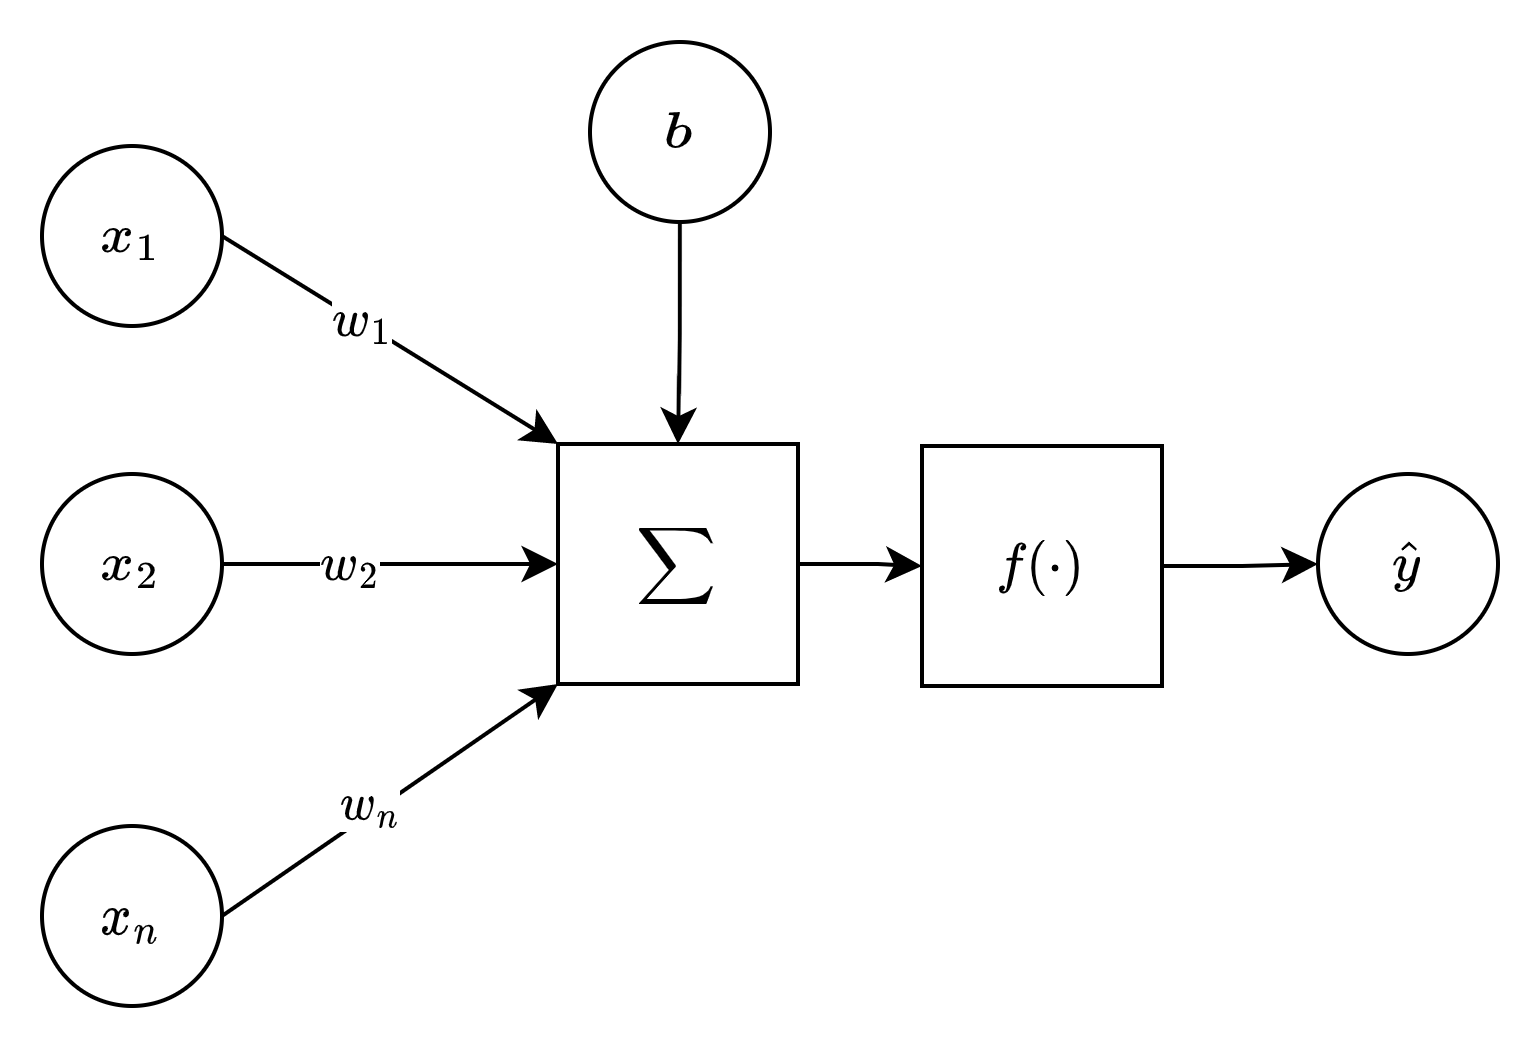
\includegraphics[width=0.4\linewidth]{figures/neuron_ai}
		\caption{Neurônio Artificial}
	\end{figure}
	
	\begin{gather*}
		\hat{y} = f( \sum_i w_i x_i + b)
	\end{gather*}
\end{frame}

%==========================================================================================
\begin{frame}
	\frametitle{Funções de Ativação}
	\begin{block}{Linear}
		\begin{itemize}
			\item $y \in [- \infty, + \infty]$
			\item Função de ativação simples
			\item Comumente usada em regressão
			\item Baixa complexidade
			\item Baixo poder de aprendizagem
		\end{itemize}
	Função:
			$$f(x) = x$$
	Derivada: 	$$\frac{\partial y}{\partial x} = 1$$
	
	\end{block}
\end{frame}

%==========================================================================================
\begin{frame}
	\frametitle{Funções de Ativação}
	\begin{alertblock}{Atenção}
		Note este caso: Porque construir modelos apenas com Lineares? \\
		input:	``10 → 100 → 200 → 10'' \\
		pesos:	``10 → 2 → 00.5 = 10 x 10 = 10'' \\
		Podemos substituir todos pesos por um só
	\end{alertblock}
	\begin{figure}
		\centering
		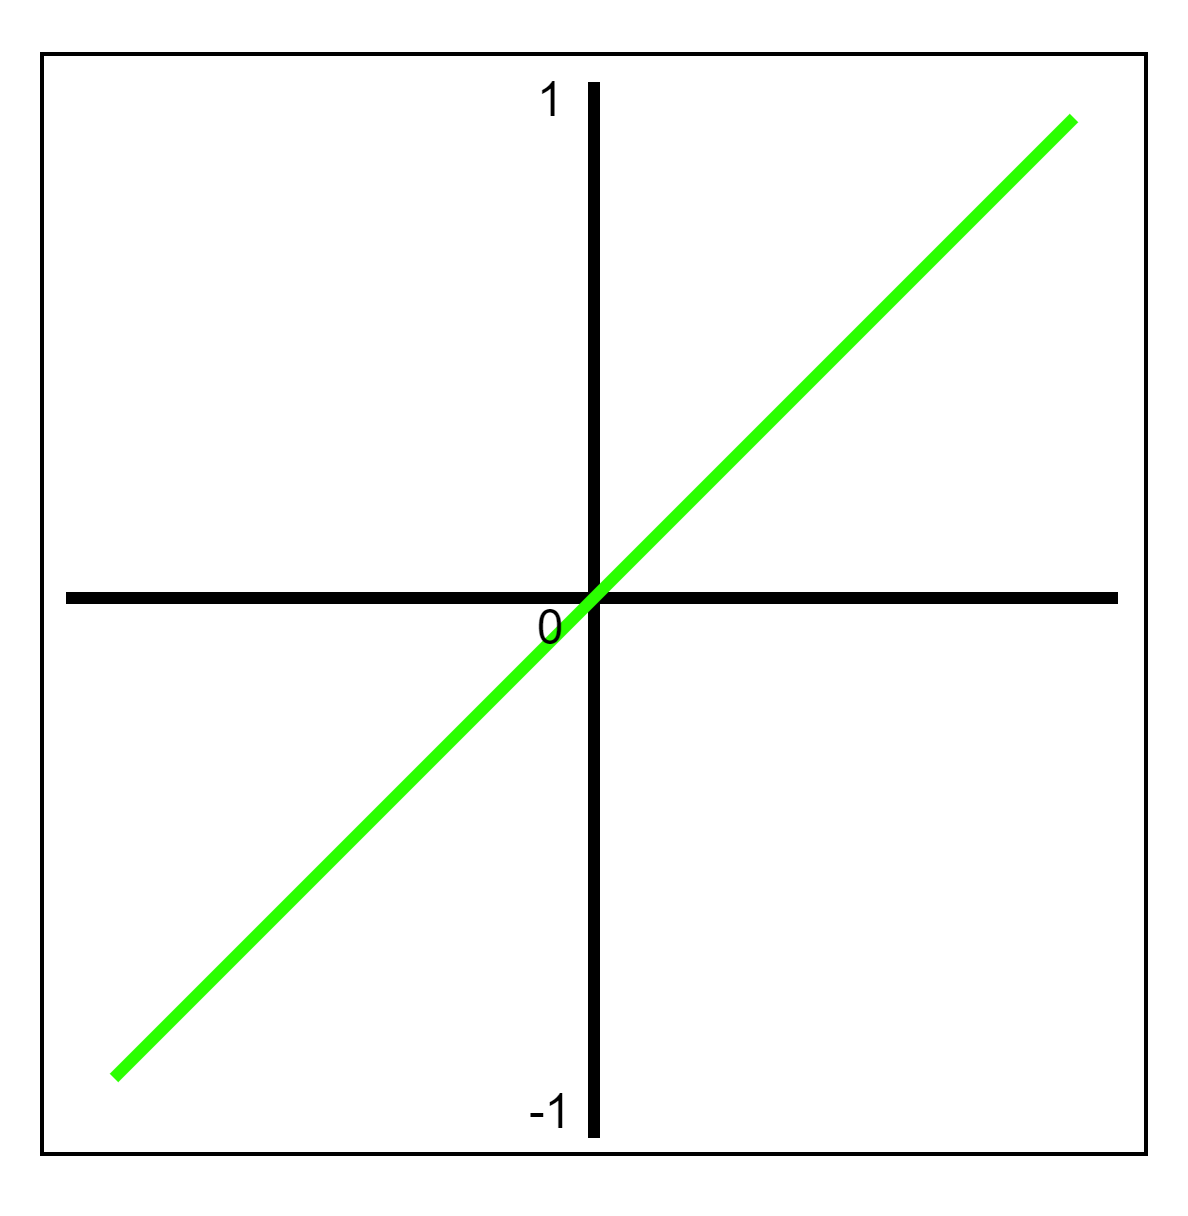
\includegraphics[width=0.4\linewidth]{figures/linear_function.png}
	\end{figure}
\end{frame}
%==========================================================================================
\begin{frame}
	\frametitle{Funções de Ativação}
	\begin{block}{Sigmoid}
		\begin{itemize}
			\item $y \in [0, + 1]$
			\item Regressão Logística
			\item Geralmente interpretada como probabilidade
			\item Saída não centrada em $0$
			\item Satura os gradientes
			\item Não indicada para camadas ocultas
			\item Converge lentamente
		\end{itemize}
		Função:
		$$f(x) = \frac{1}{1-e^{-x}}$$
		Derivada: 	$$\frac{\partial y}{\partial x} = y(1-y)$$
	\end{block}
\end{frame}
%==========================================================================================
\begin{frame}
	\frametitle{Funções de Ativação}
\begin{figure}
	\centering
	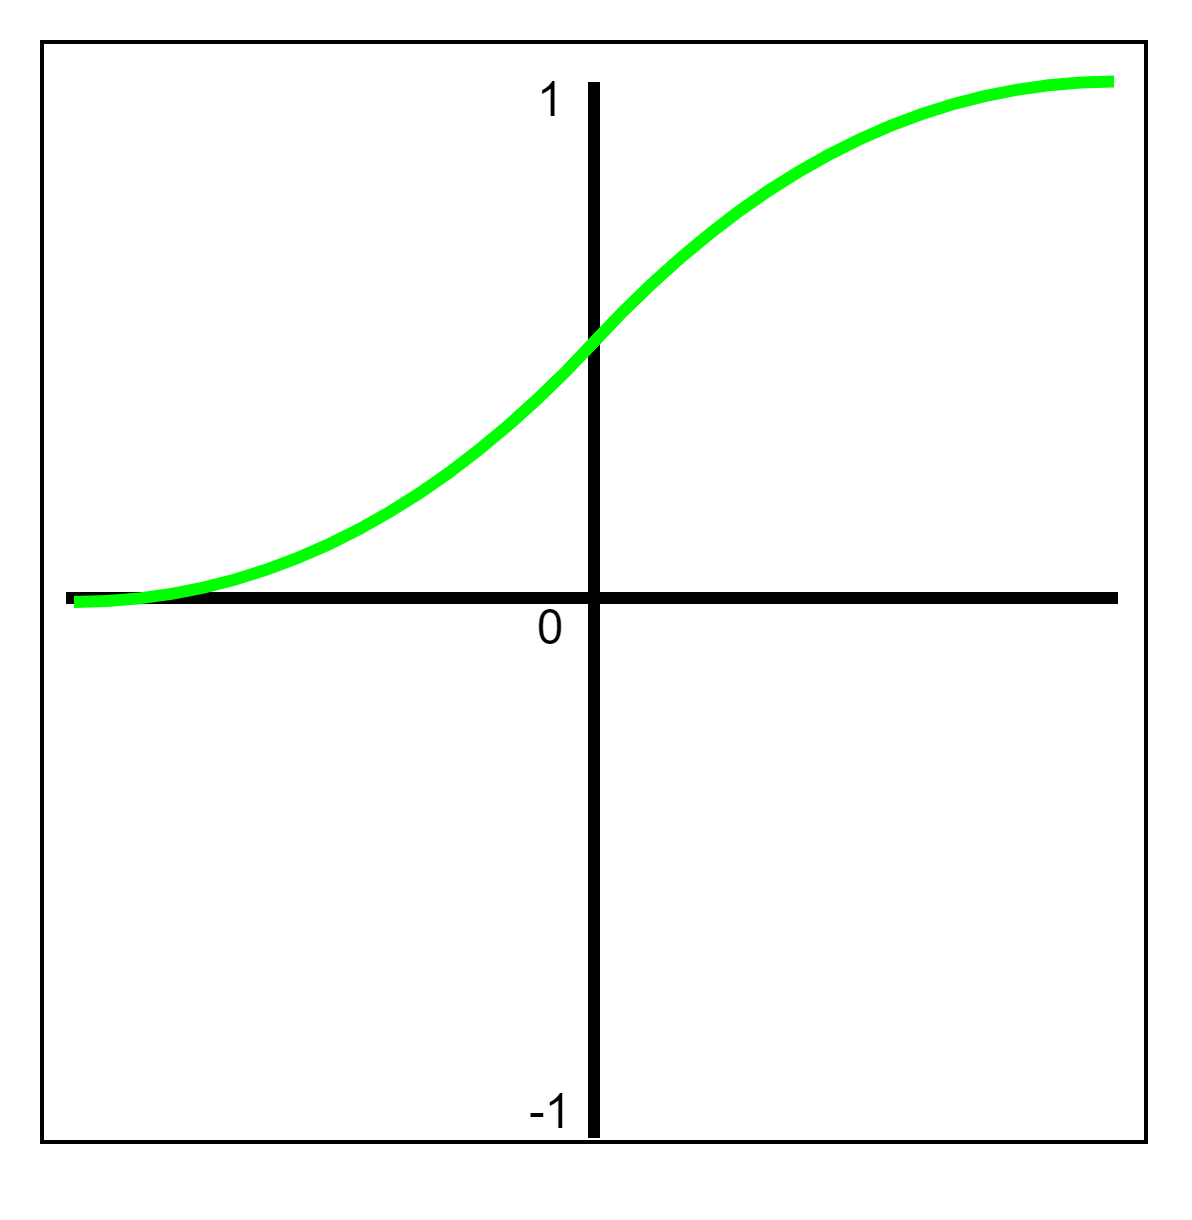
\includegraphics[width=0.4\linewidth]{figures/sigmoid_function.png}
\end{figure}
\end{frame}
%==========================================================================================
\begin{frame}
	\frametitle{Funções de Ativação}
	\begin{block}{Tanh}
		\begin{itemize}
			\item $y \in [-1, + 1]$
			\item Uma versão da Sigmoid
			\item Saída centrada em $0$
			\item Satura os gradientes. um pouco menos que a Sigmoid
			\item Converge lentamente
		\end{itemize}
		Função:
		$$f(x) = \frac{e^x - e^{-x}}{e^x+e^{-x}}$$
		Derivada: 	$$\frac{\partial y}{\partial x} = 1 - y^2$$
	\end{block}
\end{frame}
%==========================================================================================
\begin{frame}
	\frametitle{Funções de Ativação}
\begin{figure}
	\centering
	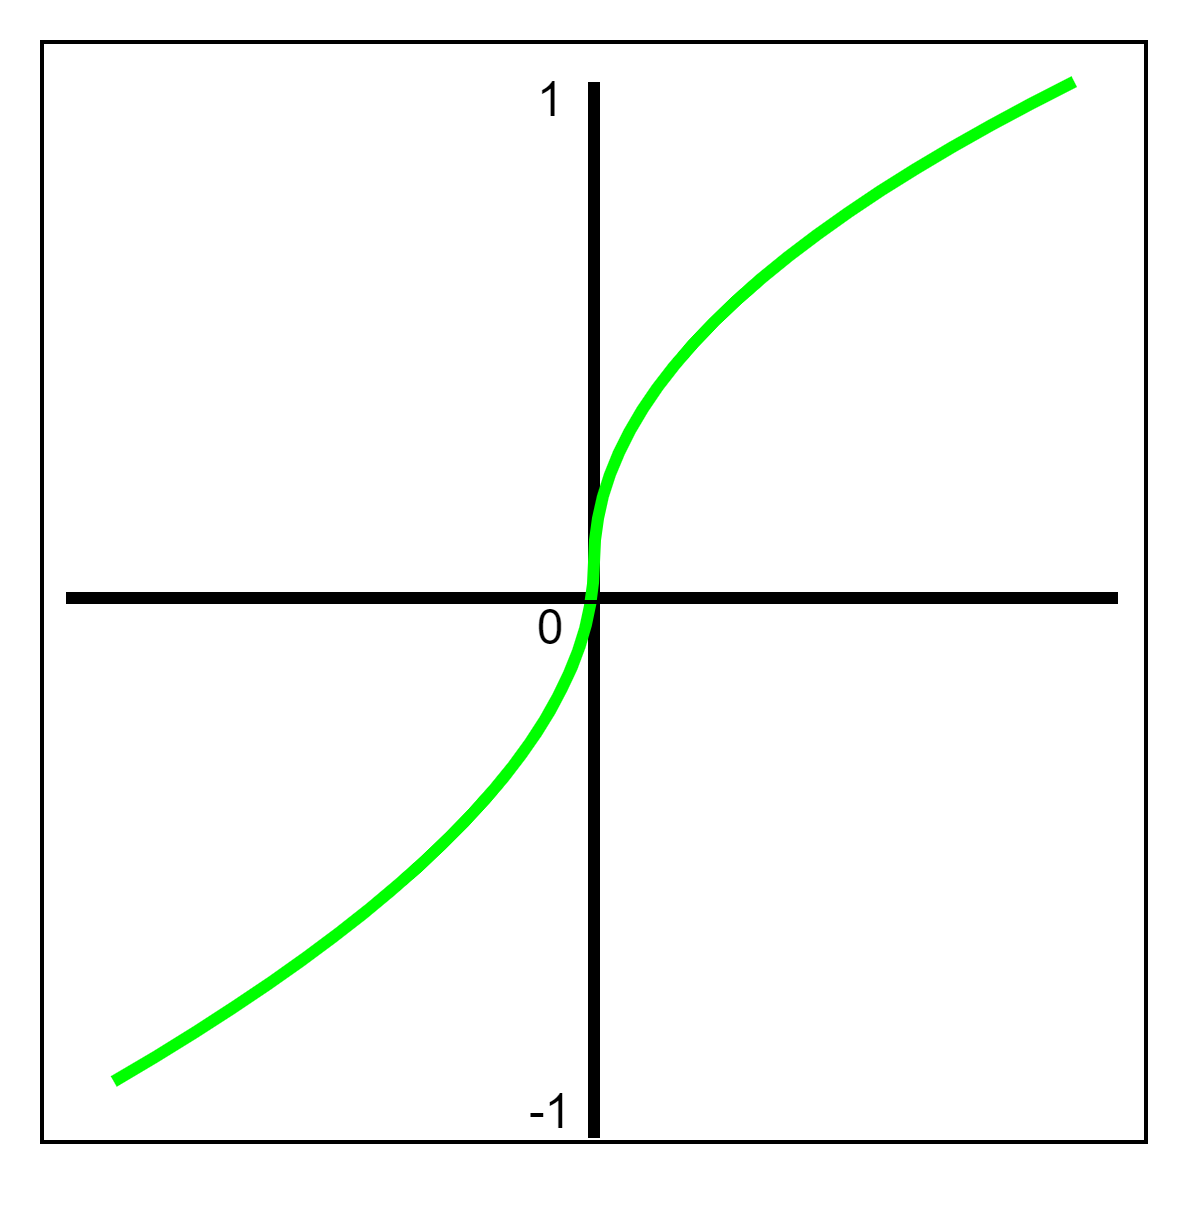
\includegraphics[width=0.4\linewidth]{figures/tanh_function}
\end{figure}
\end{frame}
%==========================================================================================
%==========================================================================================
\begin{frame}
	\frametitle{Funções de Ativação}
	\begin{block}{Relu}
		\begin{itemize}
			\item $y \in [0, + \infty]$
			\item Não tem derivada para valores $<0$
			\item Simples e Eficiente
			\item Evita a saturação dos gradientes
			\item Converge mais rápido
			\item Usada nas camadas escondidas
			\item Ela mata neurônio
		\end{itemize}
		Função:
		$$f(x) = max(0, x)$$
		Derivada: 	$$\frac{\partial y}{\partial x} =
		\left\{\begin{matrix}
			0,\; if \; x \leq 0
			\\ 
			1, \; if \; x > 0
		\end{matrix}\right.$$
	\end{block}
\end{frame}
%==========================================================================================
\begin{frame}
	\frametitle{Funções de Ativação}
	\begin{figure}
		\centering
		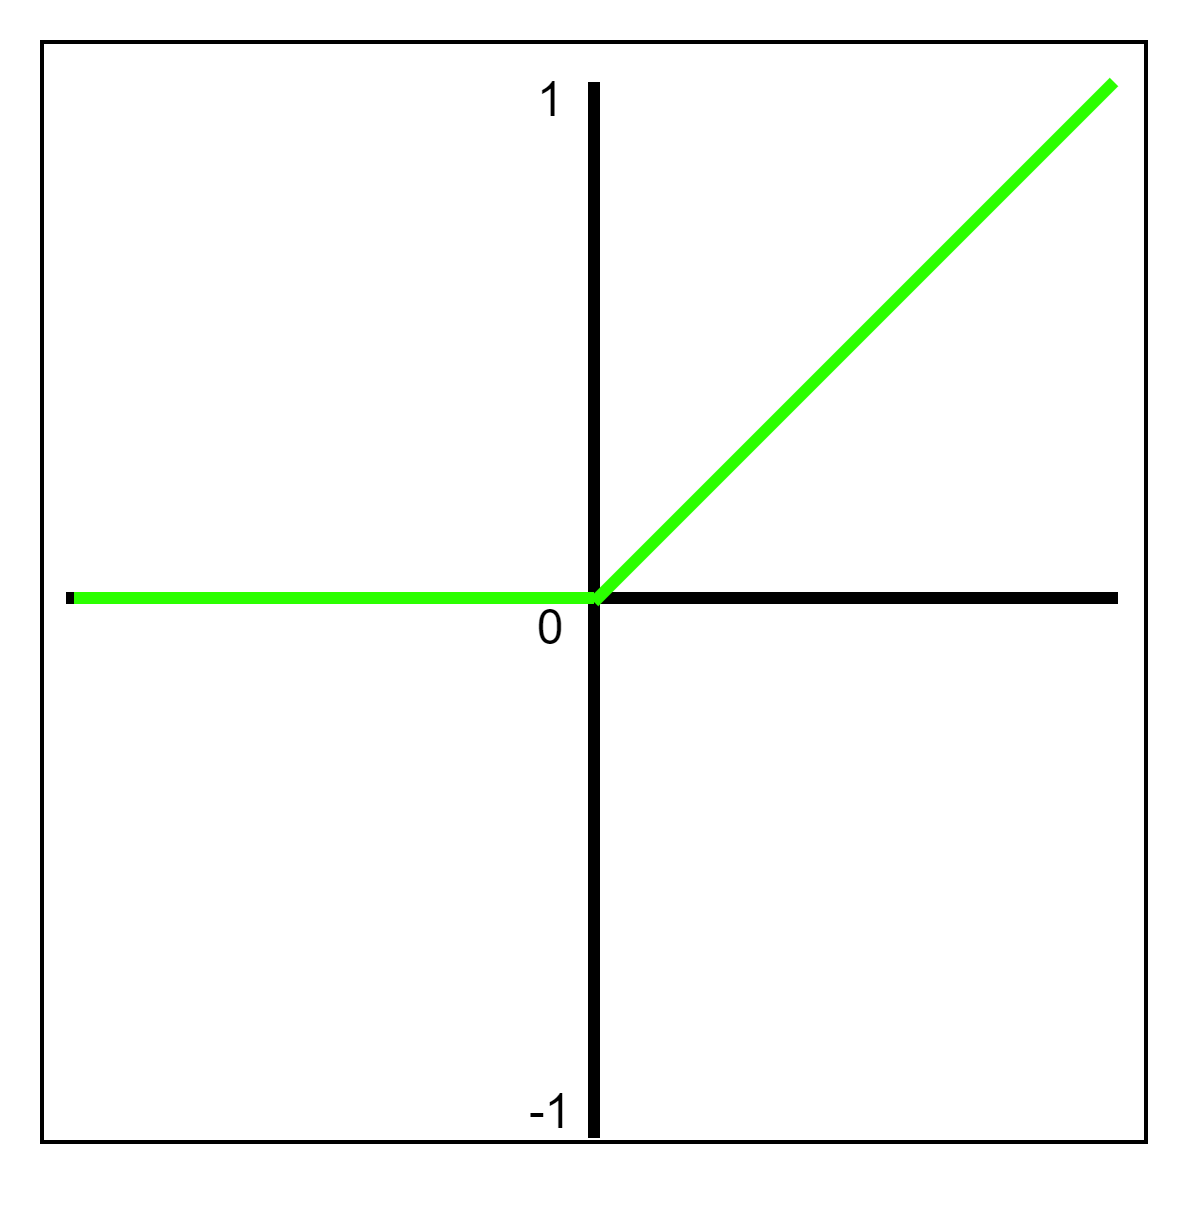
\includegraphics[width=0.4\linewidth]{figures/relu_function}
	\end{figure}
\end{frame}
%==========================================================================================
%==========================================================================================
\begin{frame}
	\frametitle{Funções de Ativação}
	\begin{block}{Leaky Relu}
		\begin{itemize}
			\item $y \in [- \infty, + \infty]$
			\item Tem derivada para valores $<0$
			\item Simples e Eficiente
			\item Evita a saturação dos gradientes
			\item Converge mais rápido
			\item Usada nas camadas escondidas
			\item Diminui as mortes de neurônios
		\end{itemize}
		Função:
		$$f(x) = 		\left\{\begin{matrix}
			\alpha(e^x - 1), x \leq 0
			\\ 
			x, x > 0
		\end{matrix}\right.$$
	
		Derivada: 	$$\frac{\partial y}{\partial x} =
		\left\{\begin{matrix}
			\alpha, x \leq 0
			\\ 
			1, x > 0
		\end{matrix}\right.$$
	\end{block}
\end{frame}
%==========================================================================================
\begin{frame}
	\frametitle{Funções de Ativação}
	\begin{figure}
		\centering
		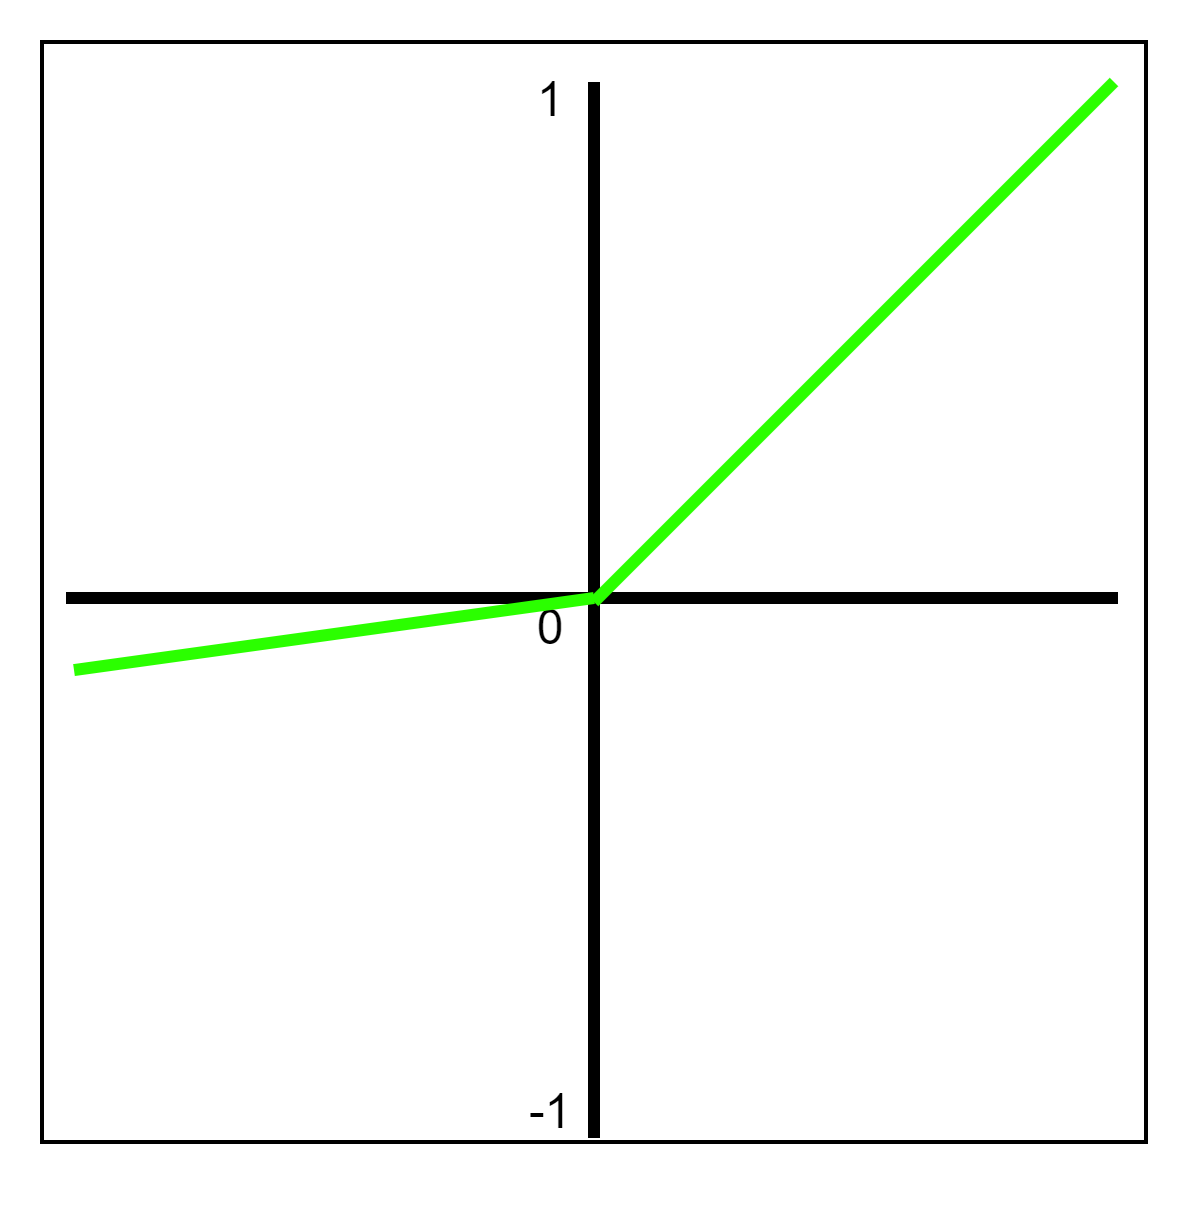
\includegraphics[width=0.4\linewidth]{figures/leaky_relu_function}
	\end{figure}
	
\end{frame}
%==========================================================================================
\begin{frame}
	\frametitle{Funções de Ativação}
	\begin{figure}
		\centering
		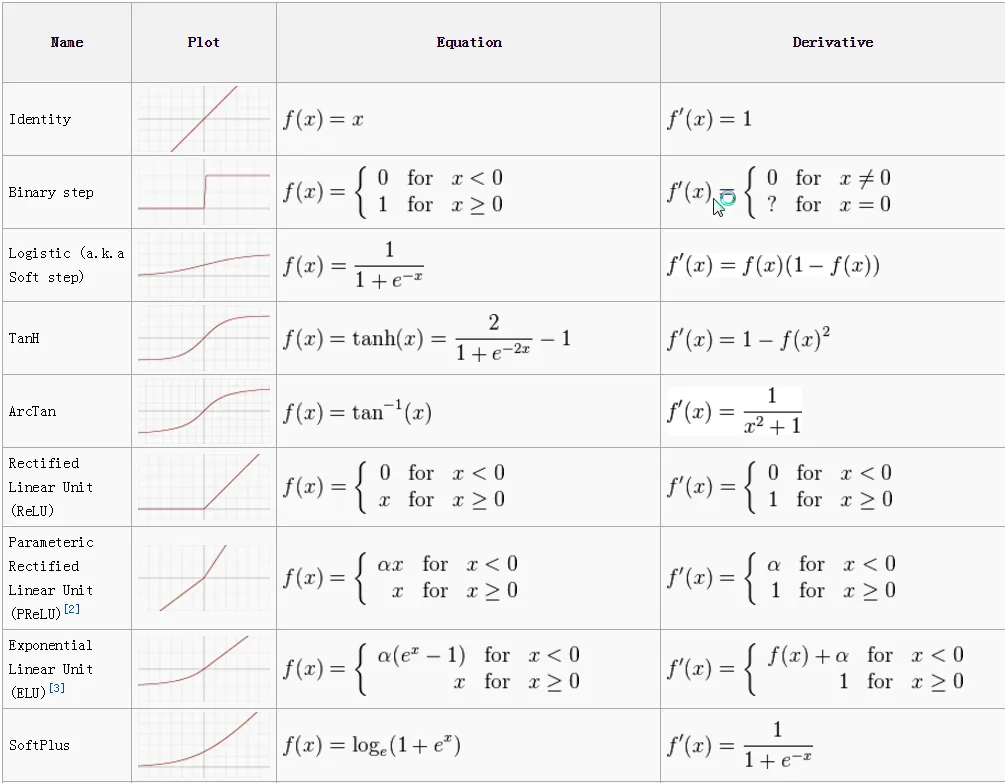
\includegraphics[width=0.7\linewidth]{figures/mais_activation_functions}
	\end{figure}

\end{frame}
%===================================================================================
%==========================================================================================
\begin{frame}
	\frametitle{Funções de Ativação}
	\begin{alertblock}{ Qual função de ativação usar?}
		\begin{itemize}
		\item	Evitar Sigmoid nas camadas ocultas, boa na saída
		\item	Tanh usada em modelos generativos
		\item	Relu Muito boa nas camadas ocultas
		\item	Linear não usar em camadas escondidas
		\item	Leaky Relu  raramente usadas
		\end{itemize}
	\end{alertblock}	
\end{frame}
%===================================================================================
\begin{frame}
	\frametitle{Funções de Ativação}
	\begin{block}{Softmax}
		\begin{itemize}
			\item $y \in [0, 1]$ e $\sum_y = 1$
			\item Aplicada em dois ou mais neurônios. Pega saída e converte
			\item A saída é uma confiança
			\item Nunca nas camadas ocultas
			\item Multiclasses
			\item Saída One-hot Encode
		\end{itemize}
		Função:
		$$S_i = \frac{e^{\hat{y}_i}}{\sum_j e^{\hat{y}_i}} $$
		Assim para cada k: $P^k = S_i^{[k]}$
		Derivada: 	$$\frac{\partial S}{\partial y} = p^k * (1-p^k)$$
	\end{block}
\end{frame}
%==========================================================================================
\begin{frame}
	\frametitle{Funções de Ativação}
	\begin{block}{Softmax}
		\begin{example}
			$[0.1, 1.3, 2.5] \to [0.07, 0.22, 0.72] $ \\
			$$\frac{e^{0.1}}{e^{0.1} + e^{0.3} + e^{2.5}}$$
		\end{example}
		Função:
		$$S_i = \frac{e^{\hat{y}_i}}{\sum_j e^{\hat{y}_i}} $$
		Assim para cada k: $P^k = S_i^{[k]}$
		Derivada: 	$$\frac{\partial y}{\partial x} =
		\left\{\begin{matrix}
			\alpha, x \leq 0
			\\ 
			1, x > 0
		\end{matrix}\right.$$
	\end{block}
\end{frame}
%==========================================================================================
%==========================================================================================
\begin{frame}
	\frametitle{Funções de Ativação}
	\begin{block}{Vamos ver na prática}
		Vamos praticar utilizando o notebook 03\_funções de ativação
	\end{block}
\end{frame}

%==========================================================================================
\section{Backpropagation}
\begin{frame}
	\frametitle{Backpropagation}
	\begin{block}{Para que usamos o \textit{backpropagation}?}
		Utilizamos o Backpropagation no treinamento das redes neurais
	\end{block}
	\begin{example}
		Vamos tomar uma função simples de multiplicação:
		$$f(x, y) = x * y$$
			
		\begin{figure}
			\centering
			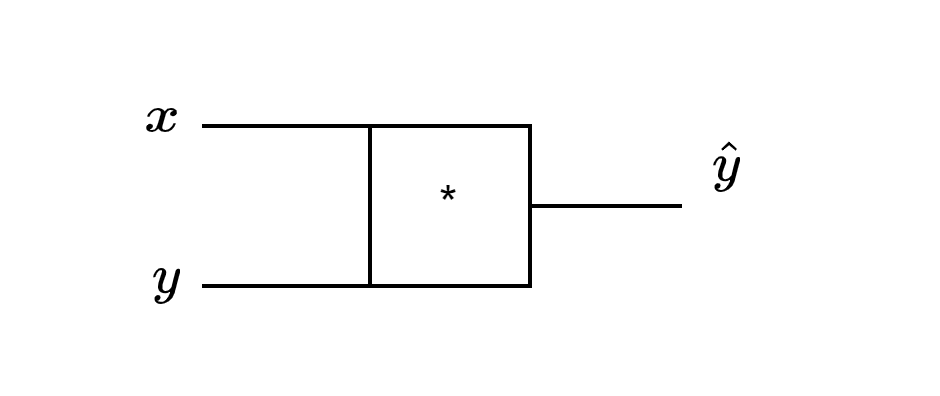
\includegraphics[width=0.5\linewidth]{figures/simple_multiply_gate}
		\end{figure}
	\end{example}
\end{frame}

%==========================================================================================
\begin{frame}
	\frametitle{Backpropagation}
	\begin{example}
		Vamos tomar uma função simples de multiplicação:
		$$f(x, y) = x * y$$
		
		\begin{figure}
			\centering
			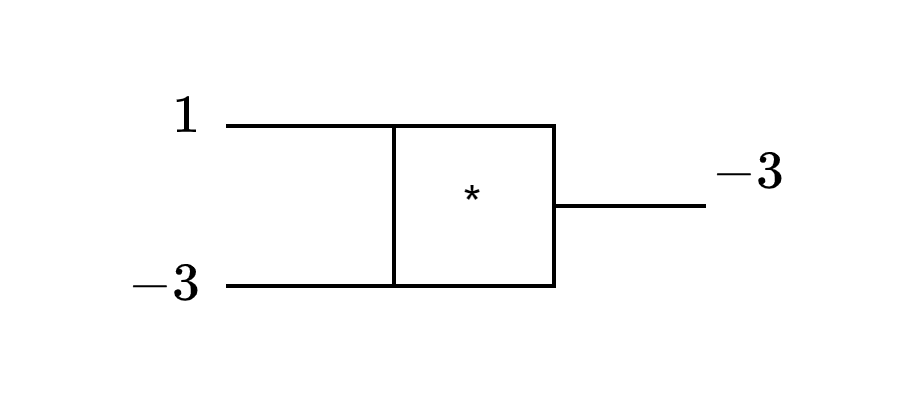
\includegraphics[width=0.5\linewidth]{figures/simple_multiply_gate_part1}
		\end{figure}
		\alert{Com que força alterar as entradas desse circuito para de maneira ``leve'' alteremos a saída?}
	\end{example}
\end{frame}
%==========================================================================================
\begin{frame}
	\frametitle{Backpropagation}
	\begin{example}
		Vamos tomar uma função simples de multiplicação:
		$$f(x, y) = x * y$$
		
\begin{figure}
	\centering
	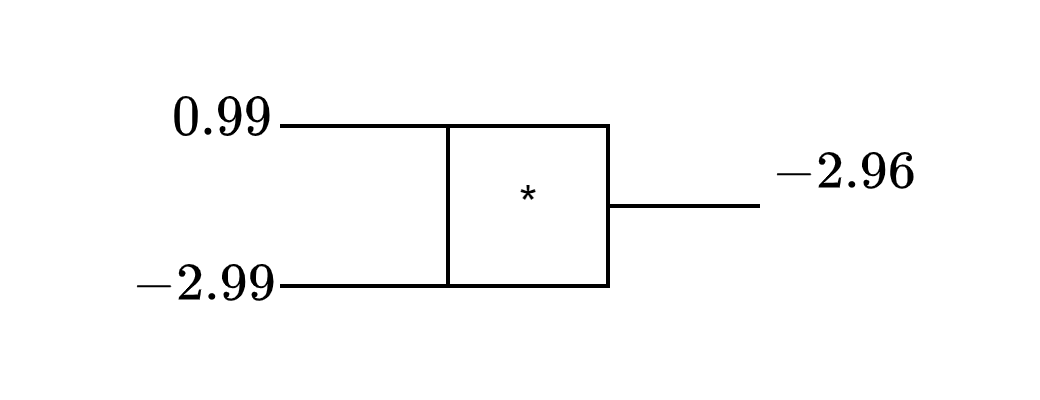
\includegraphics[width=0.5\linewidth]{figures/simple_multiply_gate_part2}
\end{figure}
		
	\end{example}
\end{frame}
%==========================================================================================
\begin{frame}
	\frametitle{Backpropagation}
	\begin{example}
		O Problema.....
		\begin{itemize}
			\item Para qual direção seguir?
			\item Com que velocidade seguir?
			\item Como sei se cheguei no local mais baixo?
		\end{itemize}
		
		\begin{figure}
			\centering
			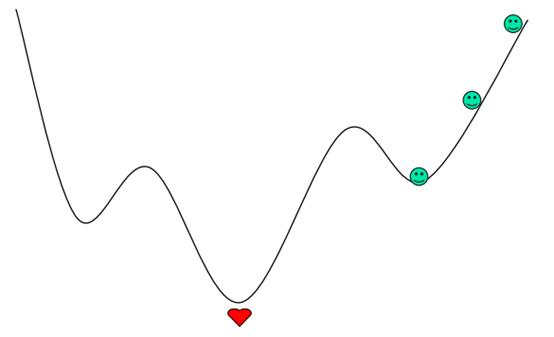
\includegraphics[width=0.5\linewidth]{figures/alpinista.png}
		\end{figure}
		
	\end{example}
\end{frame}
%==========================================================================================
\begin{frame}
	\frametitle{Backpropagation}
	\begin{block}{Vamos ver na prática}
		Vamos praticar utilizando o notebook 03\_backpropagation
		Será apresentado a busca aleatória e a busca aleatória local
	\end{block}
\end{frame}
%==========================================================================================
\begin{frame}
	\frametitle{Backpropagation}
	\begin{block}{Como atualizamos os pesos?}
		Diante disso... \\
		É possível encontrar a força de atualização dos pesos com \alert{derivadas}
		
			\href{https://github.com/mafaldasalomao/pavic_treinamento_ml/blob/main/Machine_Learning/figures/random_01.gif?raw=true}{\beamergotobutton{Figura demonstrando}} 
	\end{block}
	\begin{block}{Qual a definição básica de derivada?}
		A derivada em relação à $x$ pode ser definida como:
		$$f'(x) = \lim_{h\rightarrow 0} \frac{f(x + h) - f (x))}{h}$$
		Neste caso, o $h$ tende a $0$, ou seja, é um valor bem pequeno.
	\end{block}
\end{frame}
%==========================================================================================
%==========================================================================================
\begin{frame}
	\frametitle{Backpropagation}
	\begin{block}{Qual a definição básica de derivada parcial?}
		E se tivéssemos $n$ argumentos (componentes)? \\
		A derivada parcial de uma função com $n$ argumentos $(x_1, x_2, x_3,...,x_n)$ é dada por:
		$$\frac{\partial f}{\partial x_i}(x_1,...,x_n) = \lim_{h \rightarrow 0} \frac{f(x_1, ...,x_i + h, x_n) - f (x_1, ..., x_n))}{h}$$
		Basta derivar cada elemento, ou cada componente da função.
	\end{block}
\begin{example}
	Derivada da função $f(x) = x^2$ \\
	$$f'(x) = \lim_{h \rightarrow 0} \frac{f(x + h)-f(x)}{h}$$
\end{example}
\end{frame}
%==========================================================================================
\begin{frame}
	\frametitle{Backpropagation}
	\begin{example}
		Derivada da função $f(x) = x^2$ \\
		$$f'(x) = \lim_{h \rightarrow 0} \frac{f(x + h)-f(x)}{h}$$
		$h \rightarrow 0$ tende a zero \\
		$f(x + h)$ é p próprio $f(x)$ somado com um pequeno passo \\
		$- f(x)$ que é a própria função \\
		Dividido por $h$ normalizando a derivação \\
		$$f'(x) = \lim_{h \rightarrow 0} \frac{f(x + h)-f(x)}{h}$$
		\renewcommand{\CancelColor}{\color{red}}
		$$\frac{(x+h)^2 - x^2}{h} \rightarrow \frac{\cancel{x^2}+ 2xh +h^2 - \cancel{ x^2}}{h} \rightarrow \frac{\cancel{h}(2x + h)}{\cancel{h}} \rightarrow 2x+\cancelto{0}{h}  \rightarrow 2x$$
	\end{example}
\end{frame}
%==========================================================================================
\begin{frame}
	\frametitle{Backpropagation}
	\begin{example}
		Derivada da função $f(x) = x*y$ \\
		$$f'(x) = \lim_{h \rightarrow 0} \frac{f(x + h)-f(x)}{h}$$
		\renewcommand{\CancelColor}{\color{red}}
		$$\frac{\partial f(x,y)}{\partial x} = \frac{(x+h)y - xy}{h} = \frac{\cancel{xy} + yh - \cancel{ xy}}{h} = \frac{y\cancel{h}}{\cancel{h}} = y$$
		$$\frac{\partial f(x,y)}{\partial y} = \frac{x(y+h) - xy}{h} = \frac{\cancel{xy} + xh - \cancel{ xy}}{h} = \frac{x\cancel{h}}{\cancel{h}} = x$$
	\end{example}
\end{frame}
%==========================================================================================
\begin{frame}
	\frametitle{Backpropagation}
	\begin{block}{Mais de duas variáveis na função...}
		E se a função tiver 3 componentes?
		$f(x,y,z) = (x+y)z$
		\begin{figure}
			\centering
			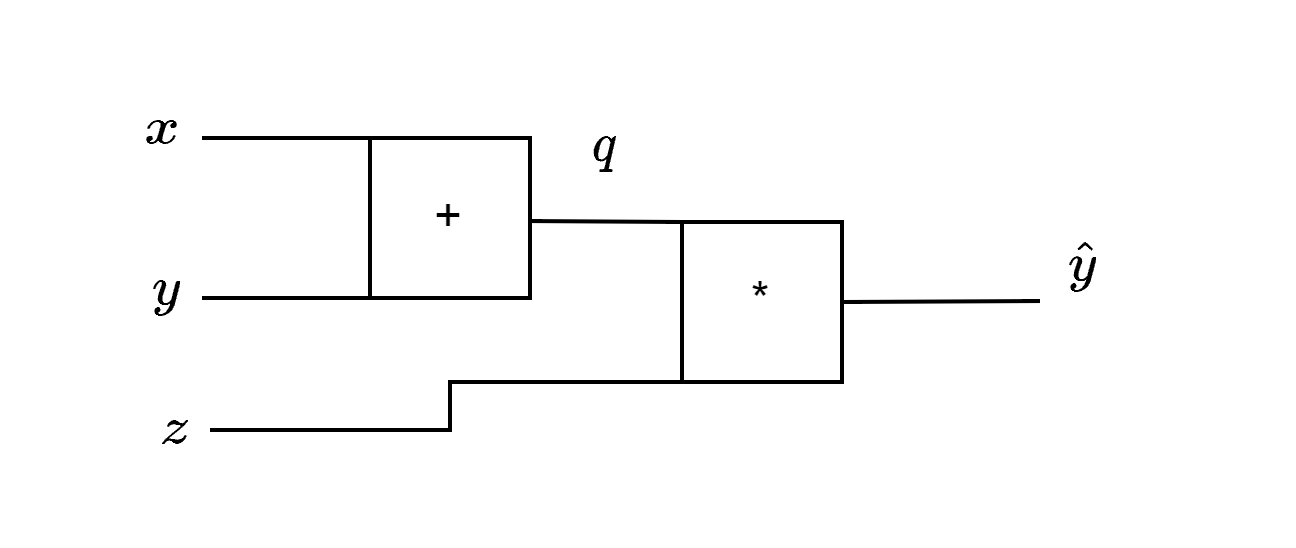
\includegraphics[width=0.7\linewidth]{figures/circuitxyz}
		\end{figure}
	Neste caso, a melhor opção é decompor a função em subfunções, ou pequenos circuitos
	\end{block}
\end{frame}
%==========================================================================================
\begin{frame}
	\frametitle{Backpropagation}
	\begin{block}{Mais de duas variáveis na função...}
		$f(x,y,z) = (x+y)z$ \\
		$q(x,y) = x+y$ \\
		$f(q,z) = qz$ \\
	\end{block}
\begin{example}
	\begin{columns}
		\begin{column}{0.35\textwidth}
			$$q(x,y) = x+y$$ \\
			$$\frac{\partial f(x,y)}{\partial x} = 1$$ \\
			$$\frac{\partial f(x,y)}{\partial y} = 1$$ \\
		\end{column}
		\begin{column}{0.35\textwidth}
			$$f(q,z) = qz$$ \\
			$$\frac{\partial f(x,y)}{\partial q} = z$$ \\
			$$\frac{\partial f(x,y)}{\partial z} = q$$ \\
		\end{column}
	\end{columns}
\end{example}
\end{frame}
%==========================================================================================
\begin{frame}
	\frametitle{Backpropagation}
	\begin{block}{Mais de duas variáveis na função...}
		Se quisermos calcular a derivada em relação a uma entrada, utilizamos a regra da cadeia: \\
		Ex: derivada em relação a $x$ de $f$
		\begin{itemize}
			\item É a derivada de $q$ em relação a $f$ 
			\item Derivada de $x$ em relação a $q$
		\end{itemize}
	\end{block}
	\begin{example}
				$$\frac{\partial f(x,y)}{\partial x} = \frac{\partial f(x,y)}{\partial q} * \frac{\partial f(x,y)}{\partial x}$$ \\
				$$\frac{\partial f(x,y)}{\partial y} = \frac{\partial f(x,y)}{\partial q} * \frac{\partial f(x,y)}{\partial y}$$ \\
				$$\frac{\partial f(x,y)}{\partial z} = q$$ 
	\end{example}
\end{frame}
%==========================================================================================
\begin{frame}
	\frametitle{Backpropagation}
	\begin{block}{Mais de duas variáveis na função...}
		Vamos verificar se dividindo a função principal em subfunções é válido.
	\end{block}
	\begin{example}
		\renewcommand{\CancelColor}{\color{red}}
		$\frac{\partial f(x,y, z)}{\partial x} = \lim_{h \rightarrow 0 }\frac{f(x+h, y,z) - f(x,y,z)}{h} = $ \\ 
		
		$ \frac{(x+h + y)*z - (x + y)*z}{h} = $ \\ $\frac{\cancel{xz}+hz + \cancel{yz} - \cancel{xz} - \cancel{yz}}{h} = $ \\ $\frac{\cancel{h}z}{\cancel{h}} = z $
	\end{example}
\end{frame}
%==========================================================================================
\begin{frame}
	\frametitle{Backpropagation}
	\begin{block}{Mais de duas variáveis na função...}
		Vamos verificar se dividindo a função principal em subfunções é válido.
	\end{block}
	\begin{example}
		\renewcommand{\CancelColor}{\color{red}}
		$\frac{\partial f(x,y, z)}{\partial y} = \lim_{h \rightarrow 0 }\frac{f(x, y+h,z) - f(x,y,z)}{h} = $ \\ 
		
		$ \frac{(x + y + h)*z - (x + y)*z}{h} = $ \\ $\frac{\cancel{xz}+hz + \cancel{yz} - \cancel{xz} - \cancel{yz}}{h} = $ \\ $\frac{\cancel{h}z}{\cancel{h}} = z $
	\end{example}
\end{frame}
%==========================================================================================
\begin{frame}
	\frametitle{Backpropagation}
	\begin{block}{Mais de duas variáveis na função...}
		Vamos verificar se dividindo a função principal em subfunções é válido.
	\end{block}
	\begin{example}
		\renewcommand{\CancelColor}{\color{red}}
		$\frac{\partial f(x,y, z)}{\partial z} = \lim_{h \rightarrow 0 }\frac{f(x, y,z+h) - f(x,y,z)}{h} = $ \\ 
		
		$ \frac{(x + y)*(z + h) - (x + y)*z}{h} = $ \\ $\frac{\cancel{xz}+xh + \cancel{yz} + yh - \cancel{xz} - \cancel{yz}}{h} = $ \\ $\frac{xh + yh}{h} =  $\\ $\frac{\cancel{h}(x + y)}{\cancel{h}} = x + y $
		
		Podemos notar que a saída é a porta de soma, ou seja. o próprio $q$
	\end{example}
\end{frame}
%==========================================================================================
\begin{frame}
	\frametitle{Backpropagation}
	\begin{block}{Vamos derivar o Neurônio Sigmoide}
		\begin{itemize}
			\item $y \in [0, + 1]$
			\item Regressão Logística
			\item Geralmente interpretada como probabilidade
			\item Saída não centrada em $0$
			\item Satura os gradientes
			\item Não indicada para camadas ocultas
			\item Converge lentamente
		\end{itemize}
		Função:
		$$f(x) = \frac{1}{1-e^{-x}}$$
	%	Derivada: 	$$\frac{\partial y}{\partial x} = y(1-y)$$
	\end{block}
\end{frame}
%==========================================================================================
\begin{frame}
	\frametitle{Backpropagation}
	\begin{block}{Vamos derivar o Neurônio Sigmoide}
		\begin{itemize}
			\item $y \in [0, + 1]$
			\item Regressão Logística
			\item Geralmente interpretada como probabilidade
			\item Saída não centrada em $0$
			\item Satura os gradientes
			\item Não indicada para camadas ocultas
			\item Converge lentamente
		\end{itemize}
		Função:
		$$f(x) = \frac{1}{1-e^{-x}}$$
		%	Derivada: 	$$\frac{\partial y}{\partial x} = y(1-y)$$
	\end{block}
\end{frame}
%==========================================================================================
\begin{frame}
	\frametitle{Backpropagation}
	\begin{block}{Vamos derivar o Neurônio Sigmoide}
		Função:
		$f(w, x) = \frac{1}{1-e^{-x}}$ \\ 
		O $w$ são os pesos e o $x$ as entradas... \\
		$f(w, x) = \frac{1}{1-e^{-(w_0x_0 + w_1x_1 + w_2)}}$
		%	Derivada: 	$$\frac{\partial y}{\partial x} = y(1-y)$$
		\begin{figure}
			\centering
			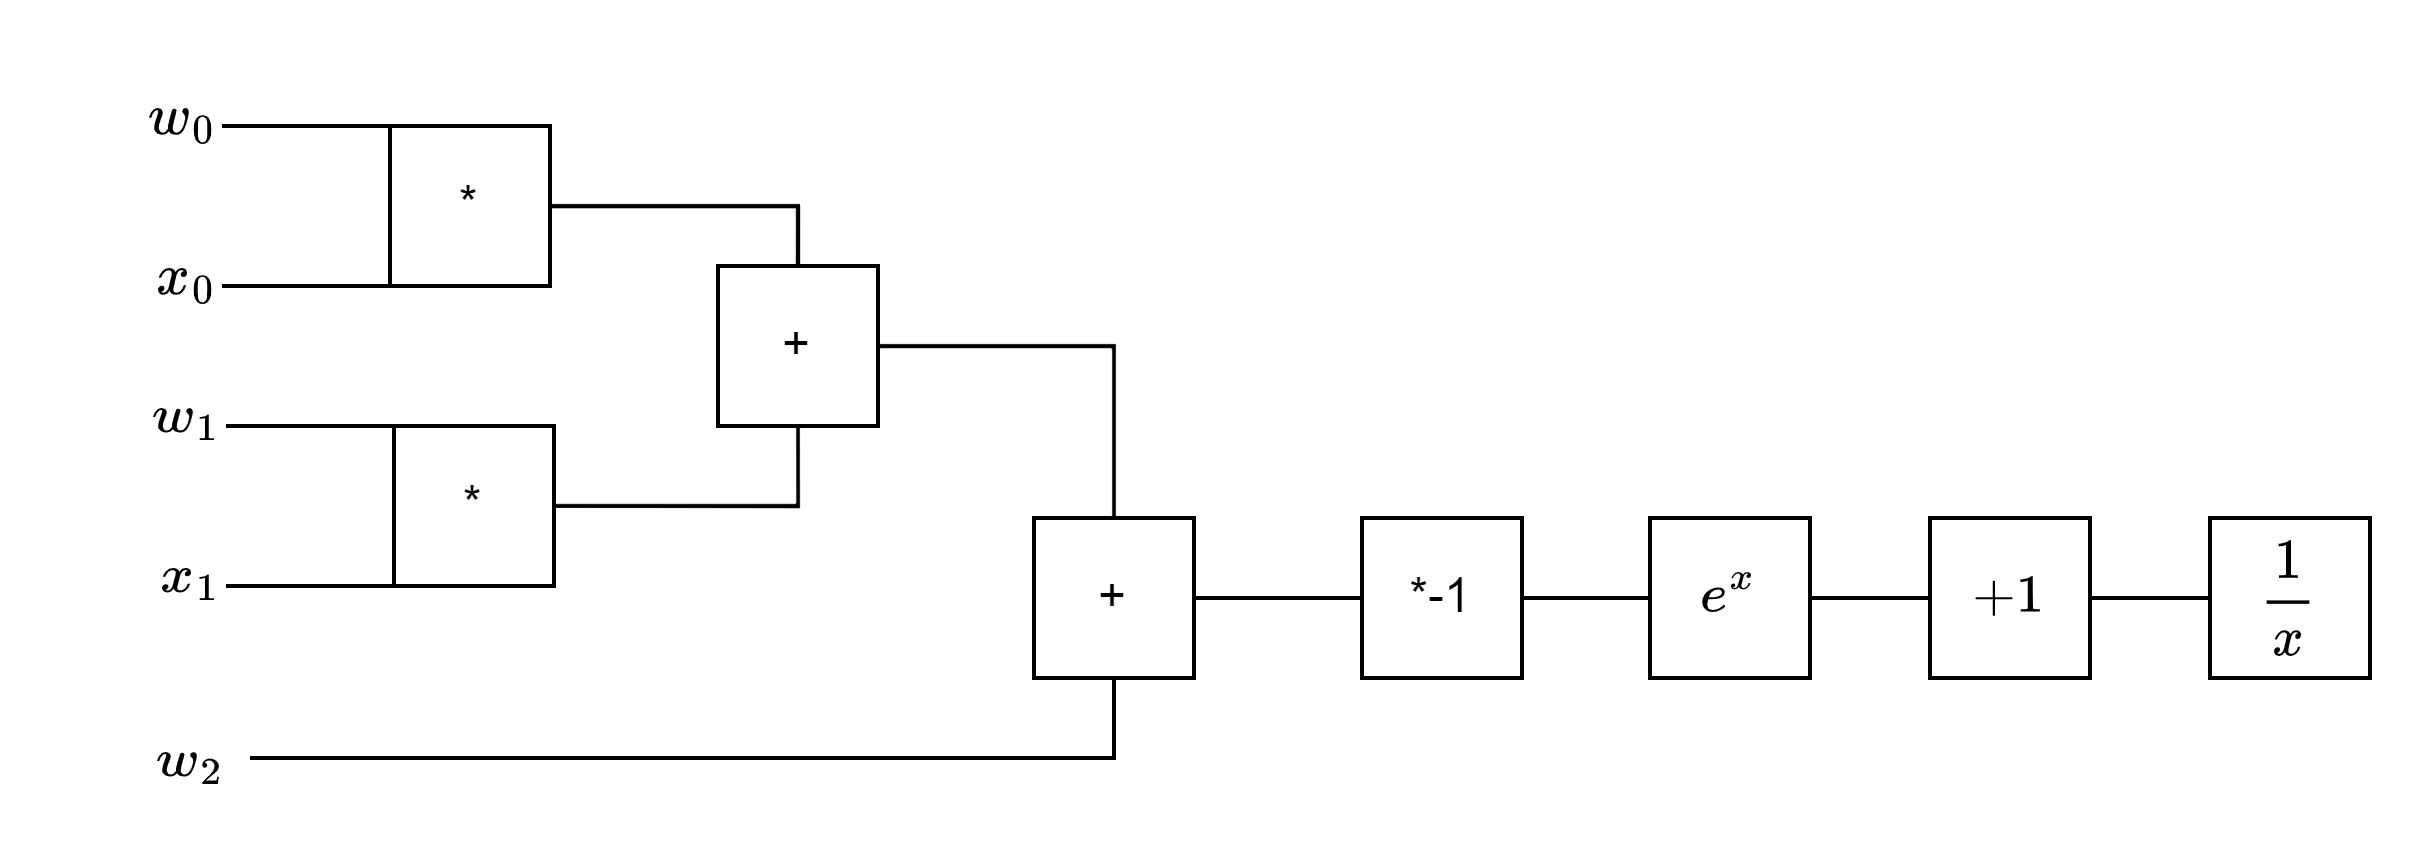
\includegraphics[width=0.7\linewidth]{figures/sigmoidneuron_derivative}
		\end{figure}
		
	\end{block}
\end{frame}
%==========================================================================================
\begin{frame}
	\frametitle{Backpropagation}
	\begin{example}
		Vamos praticar um pouquinho... \\
		A derivada de $x = a * b$ é: \\
		$da = b * dx$ \\
		Sempre teremos a derivada de dentro \alert{$da $} multiplicando a derivada de quem está fora \alert{$dx$}. Desta forma, podemos decompor qualquer função complexa. E $db = a * dx$
		\begin{columns}
			\begin{column}{0.35\textwidth}
				 $$x = a * b$$ 
				$$da = b * dx$$ 
				$$db = a * dx$$ 
			\end{column}
			\begin{column}{0.35\textwidth}
				$$x = a + b$$ 
				$$da = 1 * dx$$ 
				$$db = 1 * dx$$ 
			\end{column}
		\end{columns}
	\end{example}
\end{frame}
%==========================================================================================
\begin{frame}
	\frametitle{Backpropagation}
	\begin{example}
		Vamos ver a derivada da função $x = a + b + c$ \\
		Primeiro vamos dividir por partes: 
		$q = a+b$ e  $x = q+c$ 
		\begin{columns}
			\begin{column}{0.35\textwidth}
				$$dq = 1 * dx$$
				$$dc = 1 * dx$$
				$$db = 1 * dq$$
				$$da = 1 * dq$$
			\end{column}
			\begin{column}{0.35\textwidth}
				$$x = a + b + c$$ 
				$$da = 1 * dx$$ 
				$$db = 1 * dx$$
				$$dc = 1 * dx$$ 
			\end{column}
		\end{columns}
		Intuitivamente pode-se perceber que a derivação da soma sempre será $1 * dx$
	\end{example}
\end{frame}
%==========================================================================================
\begin{frame}
	\frametitle{Backpropagation}

		\begin{columns}
			\begin{column}{0.35\textwidth}
				\begin{example}
					$$x = a * b + c$$
					$$q = a*b dx$$ 
					$$x = q+c$$ 
					$$dq = 1 * dx$$
					$$dc = 1 * dx$$
					$$db = a * dq$$
					$$da = b * dq$$
				\end{example}
			\end{column}
			\begin{column}{0.35\textwidth}
				\begin{example}
					$$x = a * a$$ 
					$$da = 2a * dx$$
				\end{example} 
				\begin{example}
				$$x = a * a + b * b + c * c$$ 
				$$da = 2a * dx$$
				$$db = 2b * dx$$
				$$dc = 2c * dx$$
			\end{example} 
			\end{column}
		\end{columns}

\end{frame}
%==========================================================================================
\begin{frame}
	\frametitle{Backpropagation}
	\begin{example}
		Vamos ver este exemplo mais complexo
		\begin{columns}
			\begin{column}{0.35\textwidth}
				$$x = ((a * b + c) * d)^2$$
				$$x_1 = a*b+c$$ 
				$$x_2 = x_1*d$$ 
				$$x = x_2 * x_2 $$
			\end{column}
			\begin{column}{0.35\textwidth}
				$$dx_2 = 2x_2 * dx$$ 
				$$dx_1 = d * dx_2$$ 
				$$dd = x_1*dx_2$$
				$$da = b*dx_1$$
				$$db = a*dx_1$$
				$$dc = 1*dx_1$$
			\end{column}
		\end{columns}
	\end{example}
\end{frame}
%==========================================================================================
\begin{frame}
	\frametitle{Backpropagation}
		\begin{example}
			Vamos ver este exemplo de divisão
			$$x = \frac{1}{a}$$
			$$da = (-\frac{1}{a*a})*dx_1$$
		\end{example}
\end{frame}
%==========================================================================================
\begin{frame}
	\frametitle{Backpropagation}
	\begin{example}
	\begin{columns}
		\begin{column}{0.35\textwidth}
			
				$$x = \frac{a+ b}{c +d}$$
				$$x_1 = a + b$$
				$$x_2 = c + d$$
				$$x_3 = \frac{1}{x_2} $$
				$$x = x_1 * x_3$$
		\end{column}
		\begin{column}{0.35\textwidth}
			$$dx_1 = x_3 * dx$$
			$$dx_3 = x_1 * dx$$
			$$dx_2 = - \frac{1}{x_2 * x_2}*dx_3$$
			$$dc = 1 * dx_2$$
			$$dd = 1 * dx_2$$
			$$da = 1 * dx_1$$
			$$db = 1 * dx_1$$
		\end{column}
	\end{columns}
\end{example}
\end{frame}
%==========================================================================================
\begin{frame}
	\frametitle{Backpropagation}
	\begin{example}
		$$x = max(a, b)$$
		$$da = x == a ? 1 * dx : 0$$
		$$da = x == b ? 1 * dx : 0$$
		Lembram da Relu?
		$$x = max(0, a)$$
		$$da = a> 0 ? 1 * dx : 0$$
	\end{example}
\end{frame}
%==========================================================================================
\begin{frame}
	\frametitle{Backpropagation}
	\begin{block}{Como fazer derivação de matrizes}
		O que vimos até agora foram números escalares... \\
		Como derivar uma matriz?
	\end{block}
	\begin{example}	
		
		$W = np.random.randn(5, 10)$ \\
		$X = np.random.randn(3, 10)$ \\
		$Y = X.dot(W^T)$ \\
		$W$ são nossos pesos, $X$ nossas entradas, $Y$ a saída \\
		$10$ é a dimensão da entrada, $3$ Qtd de amostras, $5$ Qtd de neurônios. \\
		Anteriormente só tínhamos 1 neurônio \\ 
		A multiplicação de uma matriz de $3x10 * 10x5$ gerará uma saída $3x5$
	\end{example}
\end{frame}
%==========================================================================================
\begin{frame}
	\frametitle{Backpropagation}
	\begin{example}	
		Vamos imaginar que nosso $Y = WX$
		Se a multiplicação de uma matriz de $3x10 * 10x5$ gerará uma saída $3x5$ a derivação de $dY$ deverá ter a dimensão de $3x5$. Assim, a derivada de uma matriz sempre terá o shape da matriz original \\
		$dY = np.random.randn(*Y.shape)$ \\
		A derivada de $W$ dado $Y = WX$ será o de dentro * o de fora $X * dY$, assim: \\
		$dW = dY^T.dot(X)$\\
		A derivada de $X$ dado $Y = WX$ será o de dentro * o de fora $W * dY$, assim: \\
		$dY = dY.dot(W)$
		
		\alert{A derivada de uma matriz deverá possuir o mesmo \textit{shape} da matriz original, neste caso $Y$ tem $3x5$ e $dY$ também}
	\end{example}
\end{frame}
%==========================================================================================
\begin{frame}
	\frametitle{Backpropagation}
	\begin{block}{Resumo das derivadas}
		Vamos tomar este exemplo:
		\begin{figure}
			\centering
			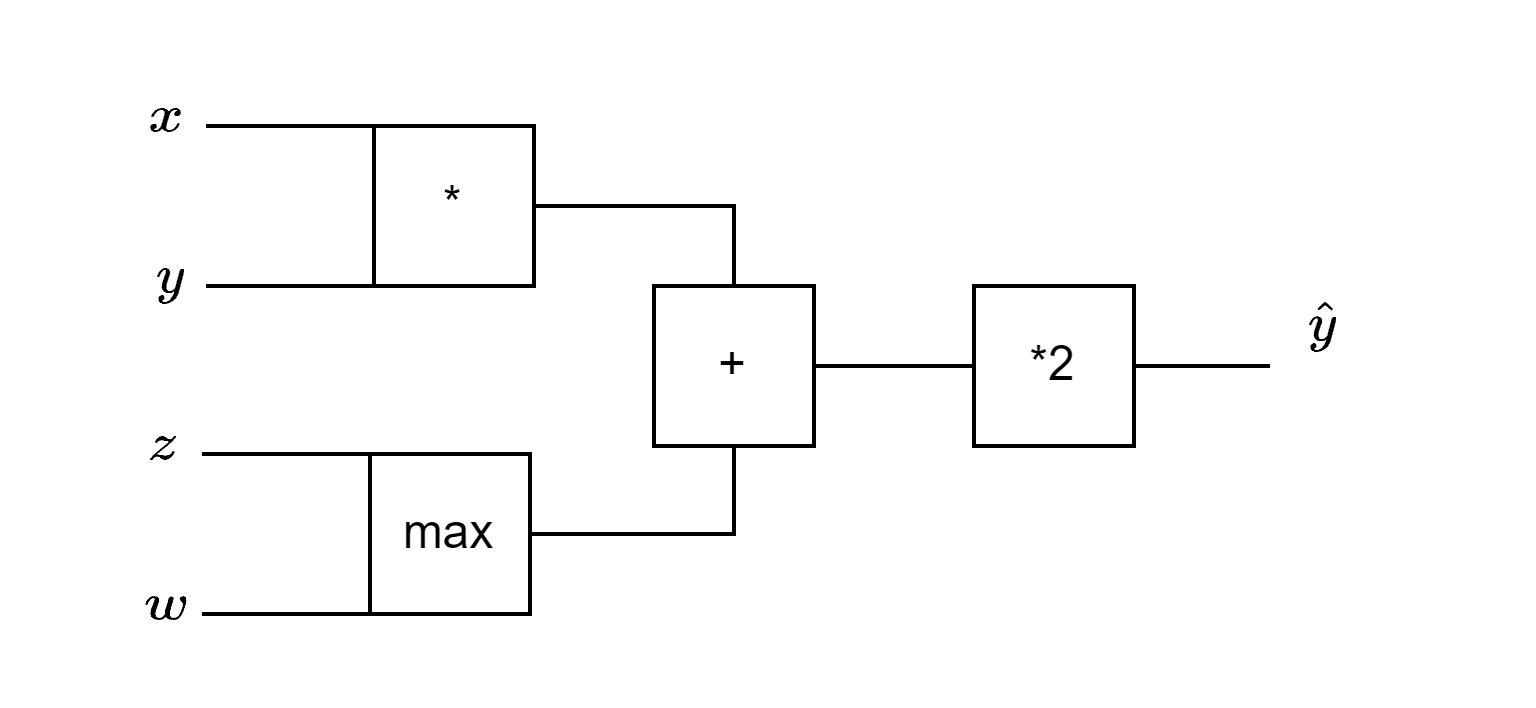
\includegraphics[width=0.7\linewidth]{figures/simple_circuit}
		\end{figure}
	\end{block}
\end{frame}
%==========================================================================================
\begin{frame}
	\frametitle{Backpropagation}
	\begin{block}{Resumo das derivadas}
		Vamos tomar este exemplo:
		\begin{figure}
			\centering
			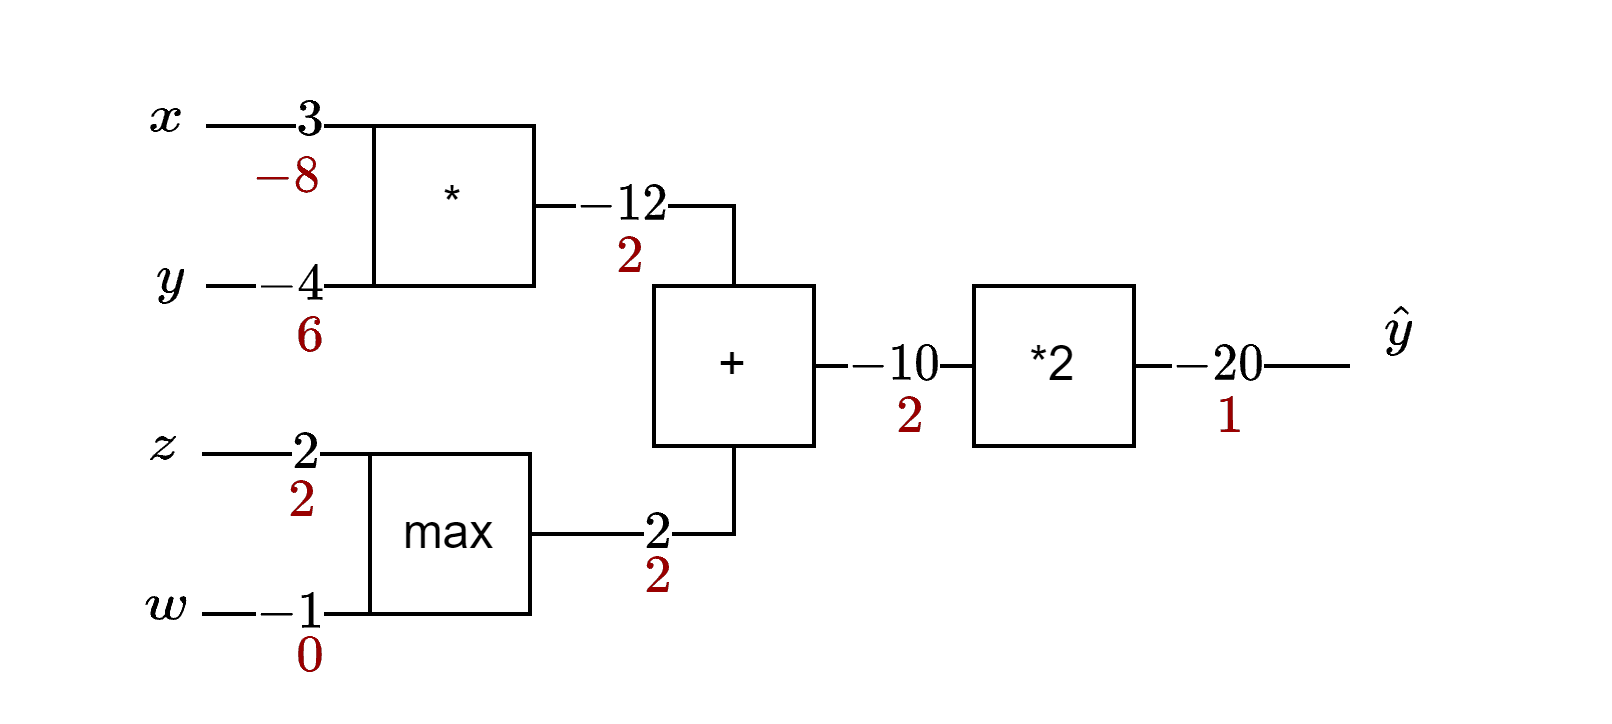
\includegraphics[width=0.7\linewidth]{figures/simple_circuit2}
		\end{figure}
	\end{block}
\end{frame}
%==========================================================================================
\begin{frame}
	\frametitle{Backpropagation}
	\begin{block}{Derivando o neurônio Sigmoide}
		Agora que sabemos como derivar, vamos retornar ao neurônio Sigmoide:
		\begin{figure}
			\centering
			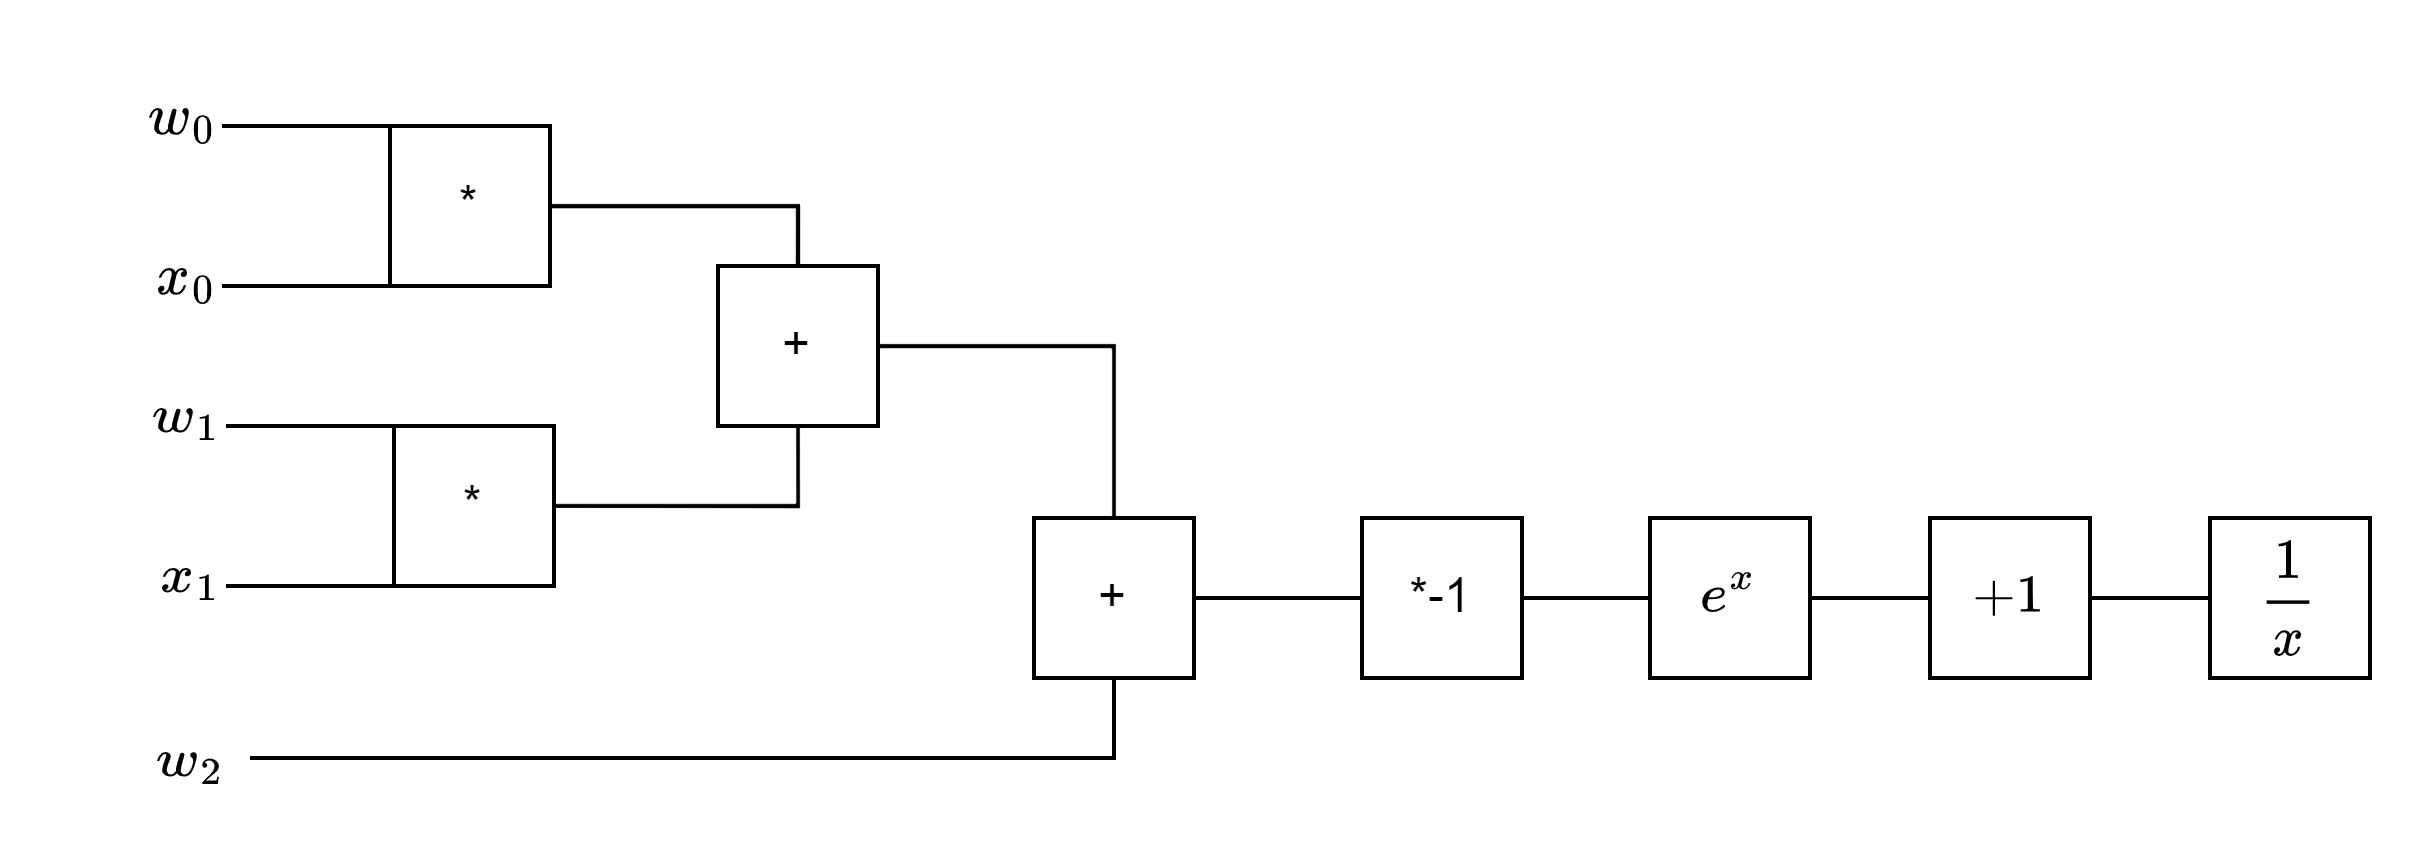
\includegraphics[width=1\linewidth]{figures/sigmoidneuron_derivative}
		\end{figure}
	\end{block}
\end{frame}
%==========================================================================================
%==========================================================================================
\begin{frame}
	\frametitle{Backpropagation}
	\begin{block}{Derivando o neurônio Sigmoide}
		Vamos fazer o processo de \textit{forward}.
		\begin{figure}
			\centering
			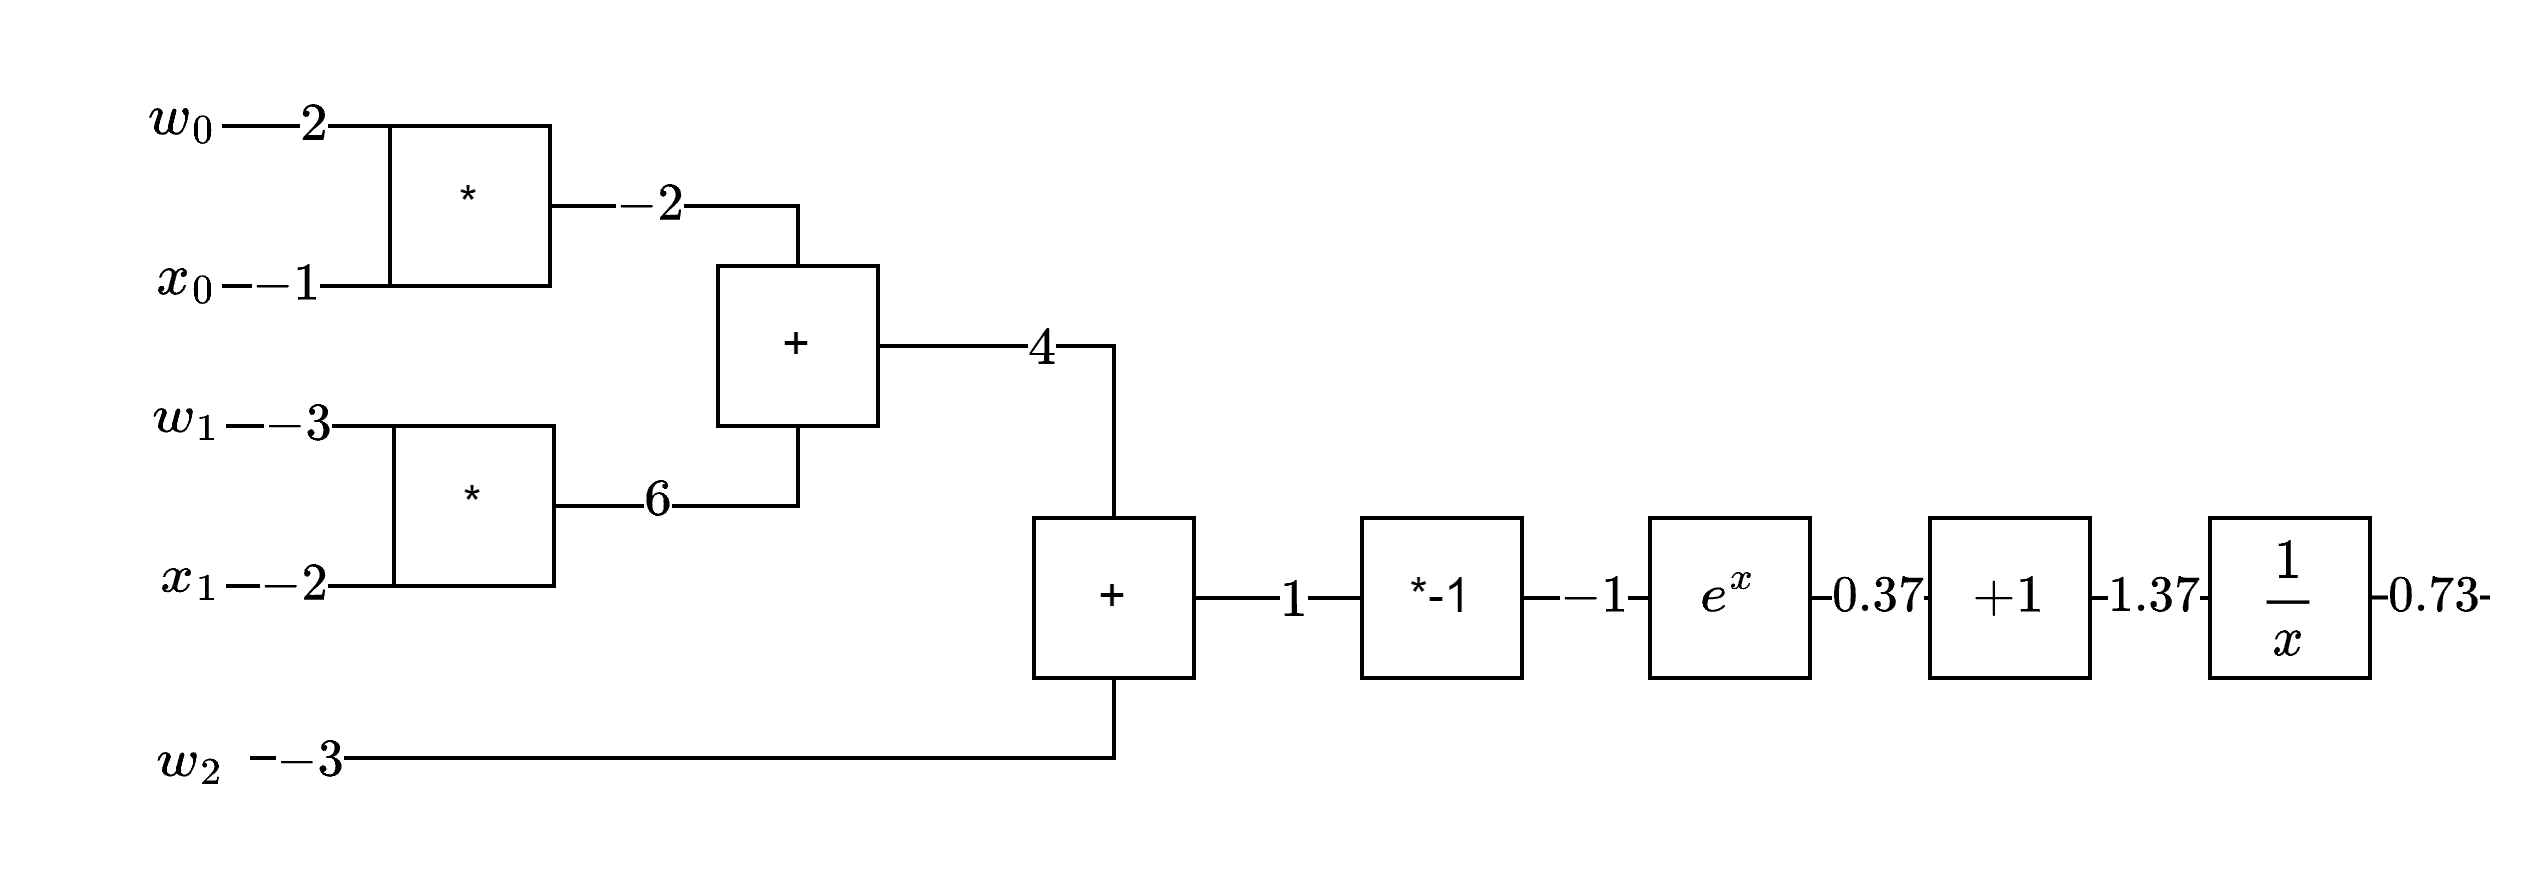
\includegraphics[width=1\linewidth]{figures/sigmoid_example}
		\end{figure}
	\end{block}
\end{frame}
%==========================================================================================
\begin{frame}
	\frametitle{Backpropagation}
	\begin{block}{Derivando o neurônio Sigmoide}
		Após o \textit{forward}, faremos agora a propagação reversa ou \textit{backpropagation}.
		\begin{figure}
			\centering
			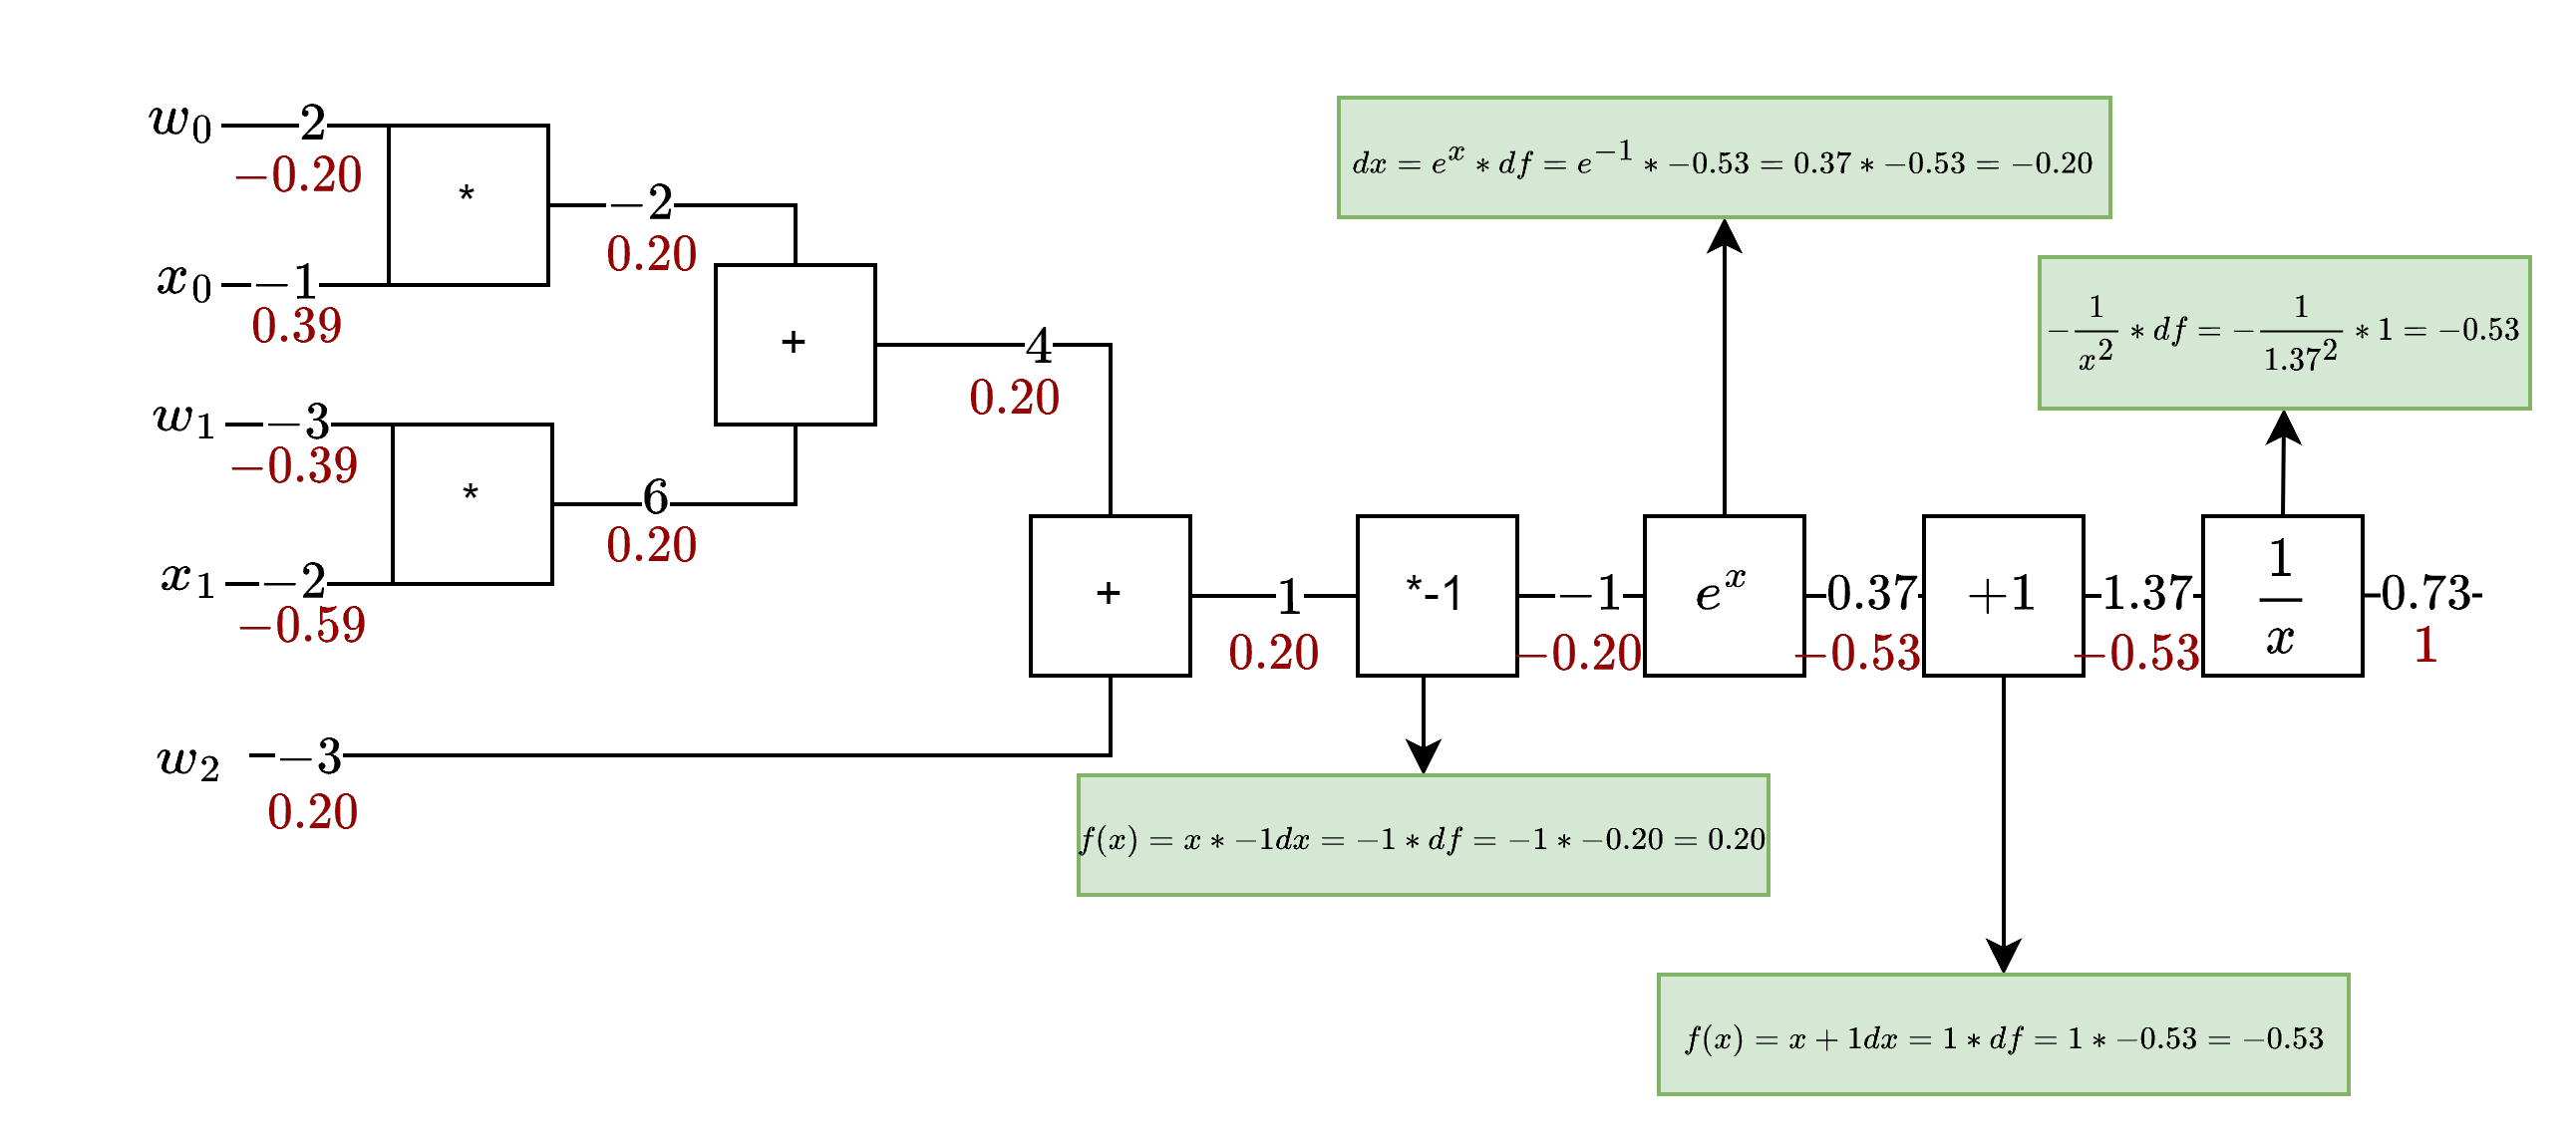
\includegraphics[width=1\linewidth]{figures/sigmoid_example_backprop}
		\end{figure}
	\end{block}
\end{frame}
%==========================================================================================
\begin{frame}
	\frametitle{Funções de Ativação}
	\begin{block}{Vamos ver na prática}
		Vamos praticar utilizando o notebook 04\_backpropagation
	\end{block}
\end{frame}
%==========================================================================================




\section{Redes Neurais Profundas}

\begin{frame}
	\frametitle{Redes Neurais Profundas}
	\begin{block}{Dimensão das matrizes}
		Até o momento vimos que um neurônio pode ser dado pela equação: $y = f(xw^T + b)$. Sendo $f$ uma função de ativação. A função de ativação não altera o \textit{shape} dos dados. \\
		A princípio tivemos $x = [1x D_{in}]$ \textit{shape}. Onde $1$ era a quantidade de amostras e $D_{in}$ o dimensões da amostra, por exemplo, a porta OR que recebe duas entradas $(x_1, x_2)$, assim $D_{in} = 2$. \\
		O mesmo ocorre para a saída, $y = [1x D_{out}]$ \textit{shape}. Onde $1$ era a quantidade de amostras e $D_{out}$ a dimensão de saída, em todos casos visto até agora igual a $1$. Mas podemos ter quantas saídas forem necessárias. \\
		Mas qual a dimensão do \textit{bias} e dos nossos pesos?
				
	\end{block}
\end{frame}

%==========================================================================================
\begin{frame}
	\frametitle{Redes Neurais Profundas}
	\begin{block}{Dimensão das matrizes}
		Assim...
		\begin{itemize}
			\item $x = [1x D_{in}]$
			\item $y = [1x D_{out}]$
			\item $bias = [1x D_{out}]$
			\item $w^T = [D_{in} x D_{out}]$
			\item $[1x D_{out}] = [1 x D_{in}] * [D_{in} x D_{out}] + [1x D_{out}]$
		\end{itemize}
	\end{block}
\end{frame}
%==========================================================================================
\begin{frame}
	\frametitle{Redes Neurais Profundas}
	\begin{block}{Dimensão das matrizes}
		\begin{columns}
			\begin{column}{0.4\textwidth}
				\begin{figure}
					\centering
					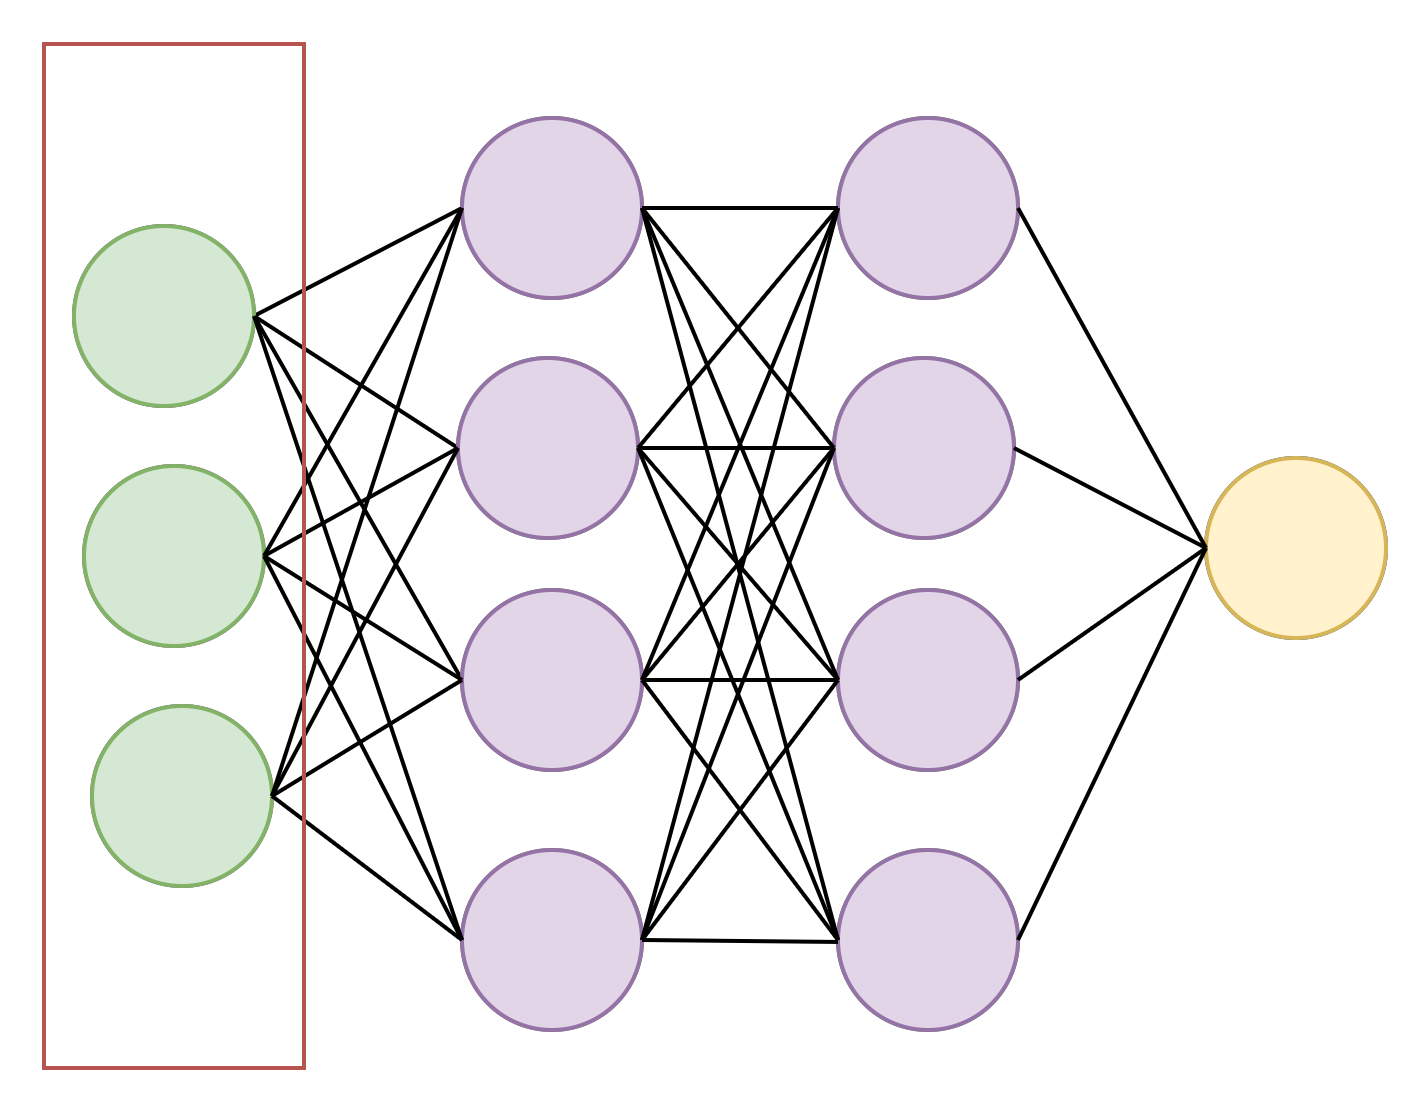
\includegraphics[width=1\linewidth]{figures/simple_nn1}
				\end{figure}
			\end{column}
			\begin{column}{0.6\textwidth}
				\begin{table}[]
					\begin{tabular}{|l|l|l|l|}
						\hline
						$[1 x D_{in}]$ & $[D_{in} x D_{out}]$ &  $[1x D_{out}]$ & $ [1x D_{out}]$ \\ \hline
						$1X3$ & $3x4$ &  $1x4$ & $1x4$  \\ \hline
					\end{tabular}
				\end{table}
			A multiplicação das matrizes $1X3 * 3x4$ nos retornará uma matriz $1x4$, que deve ser a mesma dimensão do \textit{bias}. \\
			Cada neurônio possui um bias.
			\end{column}
		\end{columns}

	\end{block}
\end{frame}
%==========================================================================================
\begin{frame}
	\frametitle{Redes Neurais Profundas}
	\begin{block}{Dimensão das matrizes}
		\begin{columns}
			\begin{column}{0.4\textwidth}
				\begin{figure}
					\centering
					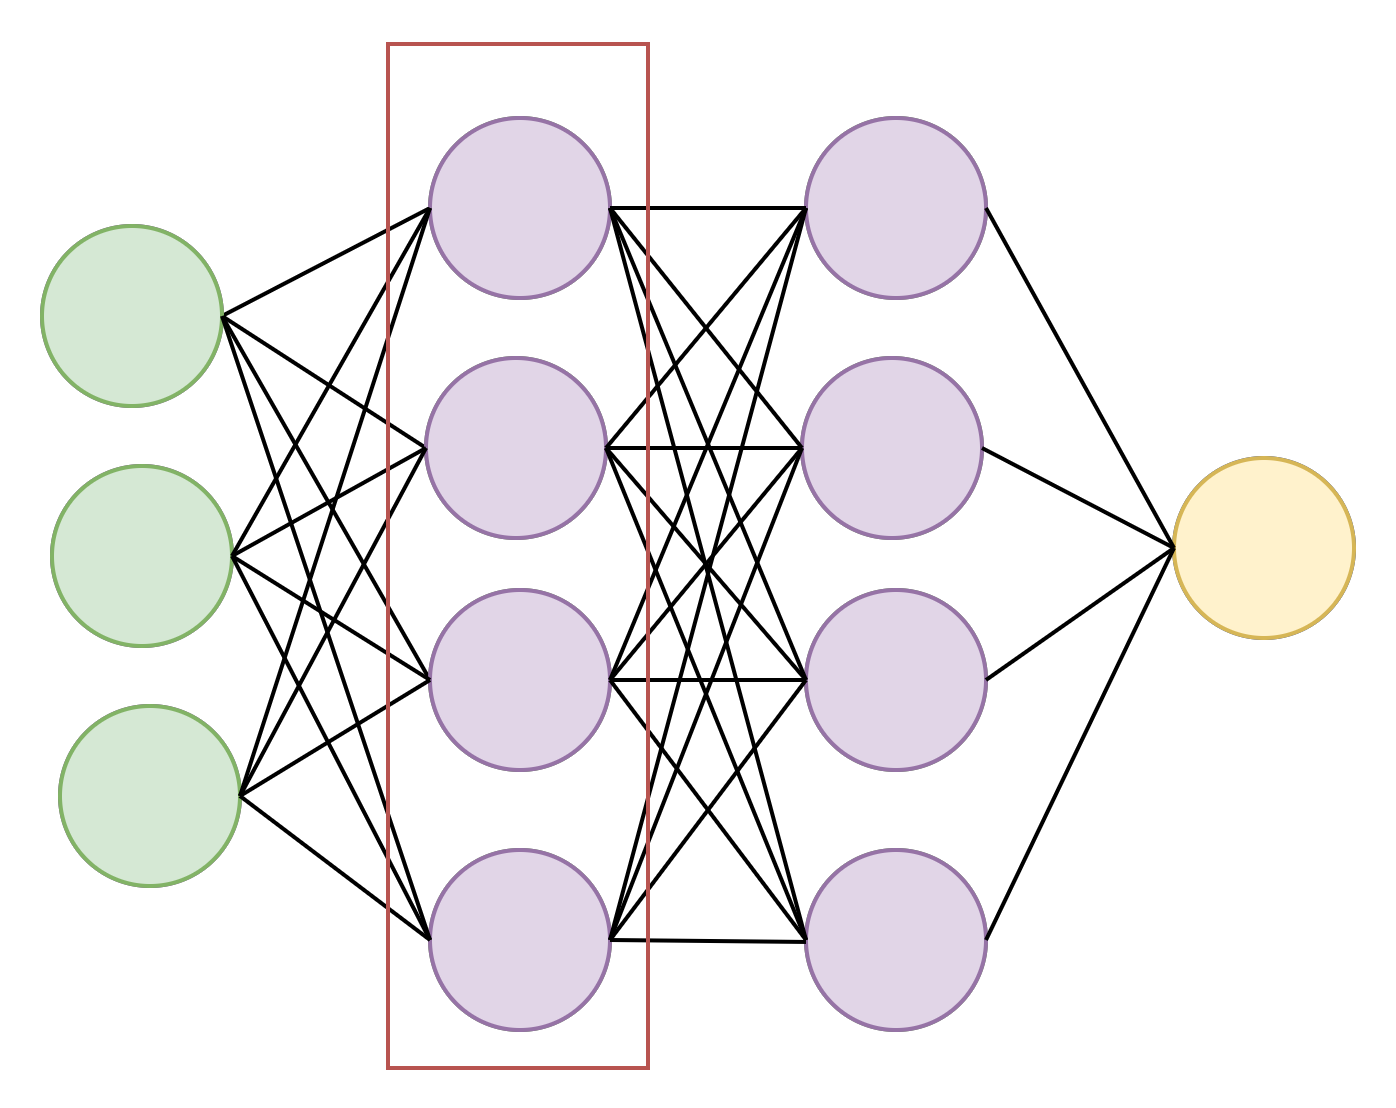
\includegraphics[width=1\linewidth]{figures/simple_nn2}
				\end{figure}
			\end{column}
			\begin{column}{0.6\textwidth}
				\begin{table}[]
					\begin{tabular}{|l|l|l|l|}
						\hline
						$[1 x D_{in}]$ & $[D_{in} x D_{out}]$ &  $[1x D_{out}]$ & $ [1x D_{out}]$ \\ \hline
						$1X3$ & $3x4$ &  $1x4$ & $1x4$  \\ \hline
						$1X4$ & $4x4$ &  $1x4$ & $1x4$  \\ \hline
					\end{tabular}
				\end{table}
				A multiplicação das matrizes $1X3 * 4x4$ nos retornará uma matriz $1x4$, que deve ser a mesma dimensão do \textit{bias}. \\
				Cada neurônio possui um bias.
			\end{column}
		\end{columns}
		
	\end{block}
\end{frame}
%==========================================================================================
\begin{frame}
	\frametitle{Redes Neurais Profundas}
	\begin{block}{Dimensão das matrizes}
		\begin{columns}
			\begin{column}{0.4\textwidth}
				\begin{figure}
					\centering
					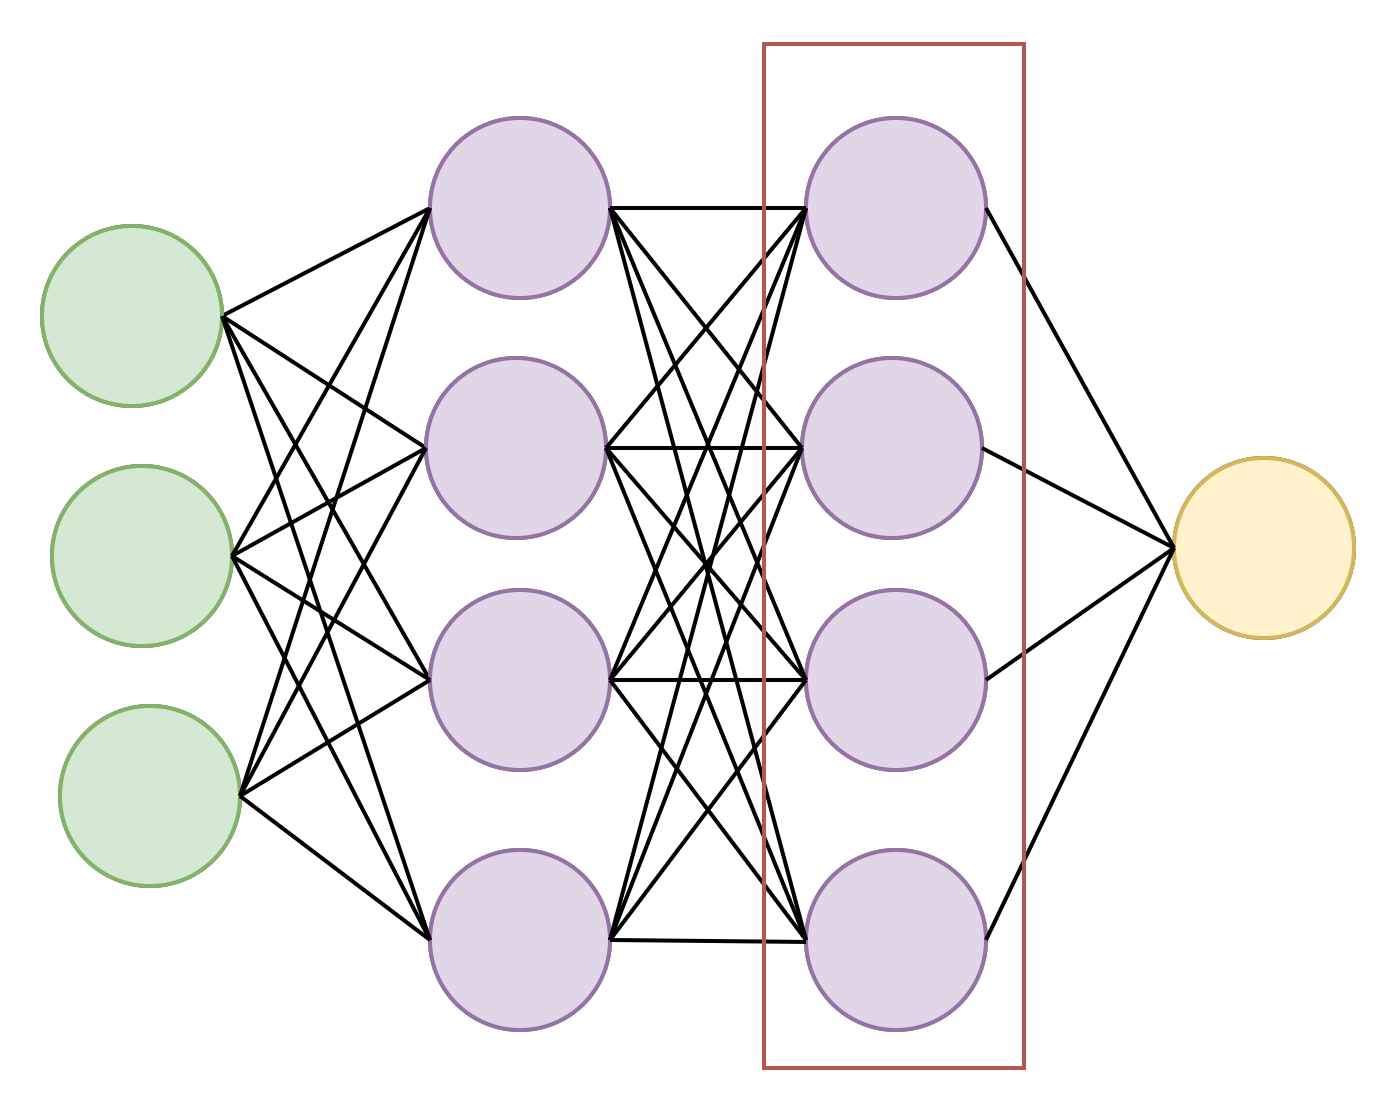
\includegraphics[width=1\linewidth]{figures/simple_nn3}
				\end{figure}
			\end{column}
			\begin{column}{0.6\textwidth}
				\begin{table}[]
					\begin{tabular}{|l|l|l|l|}
						\hline
						$[1 x D_{in}]$ & $[D_{in} x D_{out}]$ &  $[1x D_{out}]$ & $ [1x D_{out}]$ \\ \hline
						$1X3$ & $3x4$ &  $1x4$ & $1x4$  \\ \hline
						$1X4$ & $4x4$ &  $1x4$ & $1x4$  \\ \hline
						$1X4$ & $4x1$ &  $1x1$ & $1x1$  \\ \hline
					\end{tabular}
				\end{table}
				A multiplicação das matrizes $1X1 * 4x1$ nos retornará uma matriz $1x1$, que deve ser a mesma dimensão do \textit{bias}.
			\end{column}
		\end{columns}
		
	\end{block}
\end{frame}
%==========================================================================================
\begin{frame}
	\frametitle{Redes Neurais Profundas}
	\begin{block}{Dimensão das matrizes}
		\begin{columns}
			\begin{column}{0.4\textwidth}
				\begin{figure}
					\centering
					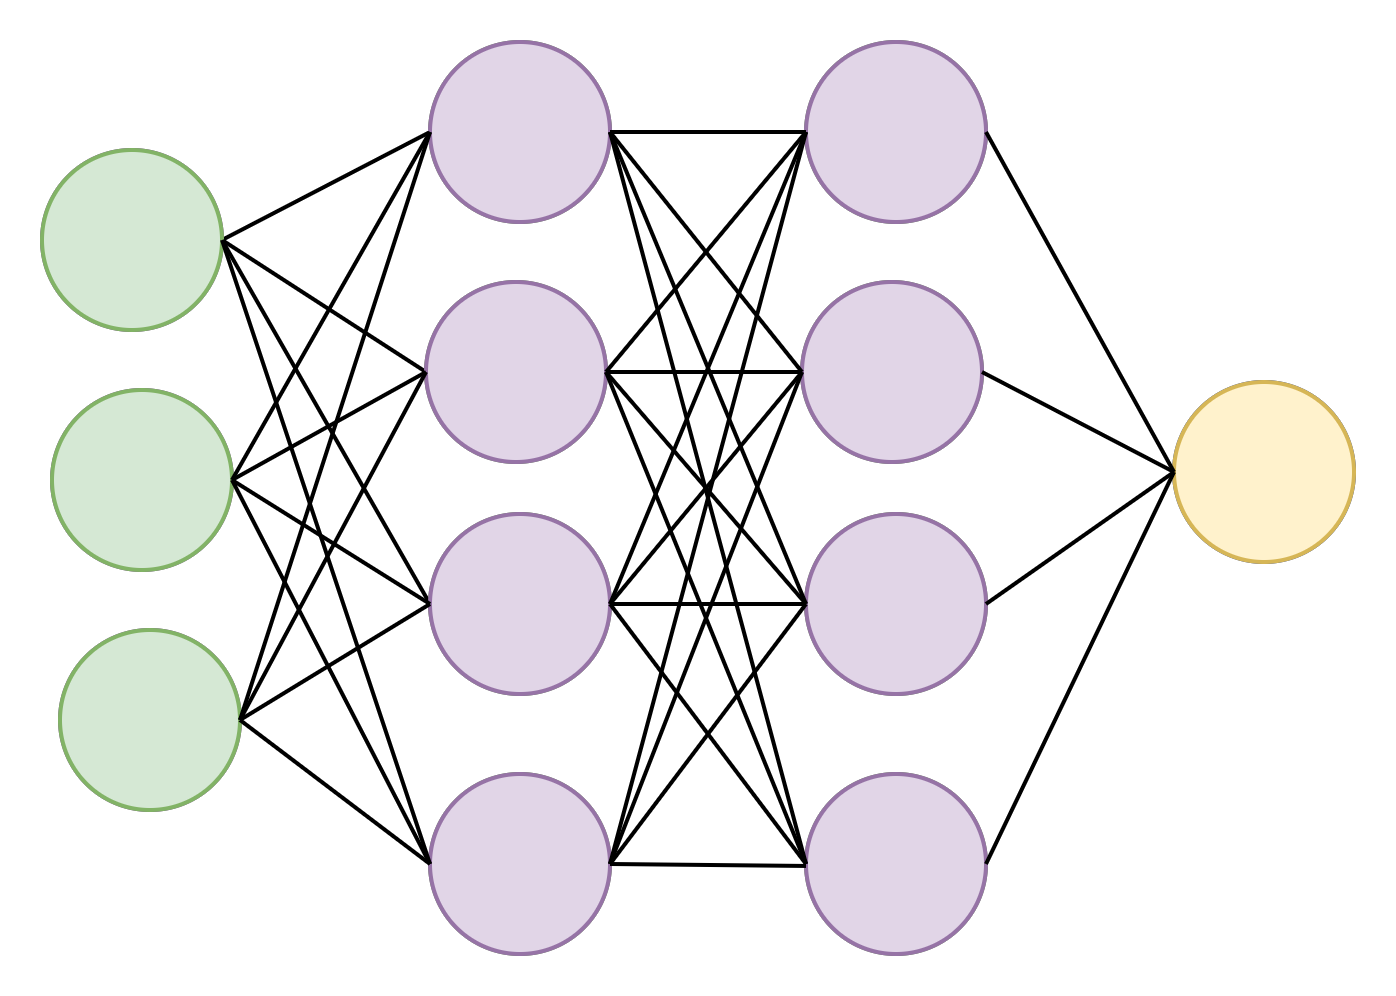
\includegraphics[width=1\linewidth]{figures/simple_nn}
				\end{figure}
			\end{column}
			\begin{column}{0.6\textwidth}
				Quantos parâmetros treináveis esta rede possui? \\
				\begin{table}[]
					\begin{tabular}{|l|l|l|l|}
						\hline
						$[1 x D_{in}]$ & $[D_{in} x D_{out}]$ &  $[1x D_{out}]$ & $ [1x D_{out}]$ \\ \hline
						$1X3$ & $3x4=\alert{12}$ &  $1x4=\alert{4}$ & $1x4$  \\ \hline
						$1X4$ & $4x4=\alert{16}$ &  $1x4=\alert{4}$ & $1x4$  \\ \hline
						$1X4$ & $4x1=\alert{4}$ &  $1x1=\alert{1}$ & $1x1$  \\ \hline
					\end{tabular}
				\end{table}
				$12 + 4 + 16 + 4 + 4 + 1 = 41$ Parâmetros
			\end{column}
		\end{columns}
	\end{block}
\end{frame}
%==========================================================================================


\section{Funções de Custo}

\begin{frame}
	\frametitle{Funções de Custo - Regressão}
		\begin{columns}
		\begin{column}{0.4\textwidth}
			\begin{block}{MAE- mean of absolute errors}
				$$J = \frac{1}{N} \sum |y_i - \hat{y}_i|$$ \\
				$$\frac{\partial J}{\partial \hat{y}} = \frac{1}{N} \left\{\begin{matrix}
					+1 se \hat{y} > y
					\\ 
					-1 se \hat{y} < y
				\end{matrix}\right.$$ 
			\end{block}
		\end{column}
		\begin{column}{0.4\textwidth}
			\begin{block}{MSE- mean of squared errors}
				$$J = \frac{1}{2N} \sum |y_i - \hat{y}_i|^2$$ \\
				$$\frac{\partial J}{\partial \hat{y}} = -(y-\hat{y})\frac{1}{N}$$ 
			\end{block}
		\end{column}
	\end{columns}
\end{frame}
%==========================================================================================

\begin{frame}
	\frametitle{Funções de Custo - Classificação binária}
	\begin{block}{Binary Cross Entropy}
		$$J = -\frac{1}{N} \sum y_iln(\hat{y}_i)+(1-y_i)ln(1-\hat{y}_i)$$ \\
		$$\frac{\partial J}{\partial \hat{y}} = \frac{-(y-\hat{y})}{\hat{y}(1-\hat{y})}\frac{1}{N}$$ 
	\end{block}
\end{frame}

%==========================================================================================

\begin{frame}
	\frametitle{One hot Encode}
	\begin{block}{One hot Encode}
		Antes de falar sobre classificação de classes, vamos entender a seguinte situação:
		\begin{columns}
			\begin{column}{0.4 \textwidth}
				\begin{table}[]
					\begin{tabular}{|l|l|}
						\hline
						y & One-hot \\ \hline
						1 & 1 0 0 0 \\ \hline
						2 & 0 1 0 0 \\ \hline
						3 & 0 0 1 0 \\ \hline
						4 & 0 0 0 1 \\ \hline
					\end{tabular}
				\end{table}
			\end{column}
			\begin{column}{0.4 \textwidth}
				\begin{table}[]
					\begin{tabular}{|l|l|}
						\hline
						y & One-hot \\ \hline
						3 & 0 0 1 0 \\ \hline
						2 & 0 1 0 0 \\ \hline
						4 & 0 0 0 1 \\ \hline
						1 & 1 0 0 0 \\ \hline
					\end{tabular}
				\end{table}
			\end{column}
		\end{columns}


	\end{block}
\end{frame}

%==========================================================================================
\begin{frame}
	\frametitle{Funções de Custo - Classificação Multiclasse}
	\begin{block}{Softmax}
		Função:
		$$S_i = \frac{e^{\hat{y}_i}}{\sum_j e^{\hat{y}_i}} $$
		Assim para cada k: $P^k = S_i^{[k]}$
		Derivada: 	$$\frac{\partial S}{\partial y} = p^k * (1-p^k)$$
	\end{block}
	\begin{alertblock}{Atenção}
		A Softmax não é uma função de custo.
	\end{alertblock}
\end{frame}
%==========================================================================================
%==========================================================================================
\begin{frame}
	\frametitle{Funções de Custo - Classificação Multiclasse}
	
	\begin{columns}
		\begin{column}{0.4 \textwidth}
		\begin{block}{Softmax}
			$$S_i = \frac{e^{\hat{y}_i}}{\sum_j e^{\hat{y}_i}} $$
			Assim para cada k: $P^k = S_i^{[k]}$
			Derivada: 	$$\frac{\partial S}{\partial y} = p^k * (1-p^k)$$
		\end{block}
		\end{column}
		\begin{column}{0.4 \textwidth}
		\begin{block}{Neg. Log-likelihood}
			$$J = \frac{1}{N} \sum -ln(p_i^k) $$
			 $$\frac{\partial J}{\partial p^k} = - \frac{1}{p^k}$$
			Derivada: 	$$\frac{\partial J}{\partial \hat{y}} = -(1-p^k) = -(y-\hat{y}) \frac{1}{N}$$
		\end{block}
		\end{column}
	\end{columns}
	\begin{alertblock}{Atenção}
		A Neg. Log-likelihood será o somatório do logarítmico  da negação para cada elemento da Softmax pelo total de elementos.
	\end{alertblock}
\end{frame}
%==========================================================================================
\begin{frame}
	\frametitle{Funções de Custo}
	\begin{block}{Qual função de custo utilizar?}
	\begin{table}[]
		\begin{tabular}{c|ccc|}
			\cline{2-4}
			& \multicolumn{3}{c|}{Problema}                                             \\ \hline
			\multicolumn{1}{|c|}{} &
			\multicolumn{1}{c|}{Regressão} &
			\multicolumn{1}{c|}{\begin{tabular}[c]{@{}c@{}}Classificação\\ Binária\end{tabular}} &
			\begin{tabular}[c]{@{}c@{}}Classificação\\ Multiclasse\end{tabular} \\ \hline
			\multicolumn{1}{|c|}{\begin{tabular}[c]{@{}c@{}}\#neurônios\\ ult. camada\end{tabular}} & \multicolumn{1}{c|}{\#outputs} & \multicolumn{1}{c|}{1}       & \#classes \\ \hline
			\multicolumn{1}{|c|}{\begin{tabular}[c]{@{}c@{}}F. Ativação\\ ult. camada\end{tabular}} & \multicolumn{1}{c|}{Linear}    & \multicolumn{1}{c|}{Sigmoid} & Linear    \\ \hline
			\multicolumn{1}{|c|}{F. de Custo} &
			\multicolumn{1}{c|}{\begin{tabular}[c]{@{}c@{}}MSE, MAE,\\ SSE, ...\end{tabular}} &
			\multicolumn{1}{c|}{Cross Entropy} &
			\begin{tabular}[c]{@{}c@{}}Softmax +\\ Neg. Log-Likelihood\end{tabular} \\ \hline
		\end{tabular}
	\end{table}
	\end{block}
\end{frame}

%==========================================================================================

%==========================================================================================
\begin{frame}
	\frametitle{Funções de Ativação}
	\begin{block}{Vamos ver na prática}
		Vamos praticar utilizando o notebook 05\_redesneuraisintuicao
	\end{block}
\end{frame}
%==========================================================================================

\section{Rede Neural do Zero}

\begin{frame}
	\frametitle{Funções de Custo - Regressão}
	\begin{block}{Passo 1}
		Primeiramente vamos implementar nossas funções de custo... \\
		Será Utilizado o notebook 06\_rede neural
	\end{block}
	\begin{columns}
		\begin{column}{0.4\textwidth}
			\begin{block}{MAE- mean of absolute errors}
				$$J = \frac{1}{N} \sum |y_i - \hat{y}_i|$$ \\
				$$\frac{\partial J}{\partial \hat{y}} = \frac{1}{N} \left\{\begin{matrix}
					+1 se \hat{y} > y
					\\ 
					-1 se \hat{y} < y
				\end{matrix}\right.$$ 
			\end{block}
		\end{column}
		\begin{column}{0.4\textwidth}
			\begin{block}{MSE- mean of squared errors}
				$$J = \frac{1}{2N} \sum |y_i - \hat{y}_i|^2$$ \\
				$$\frac{\partial J}{\partial \hat{y}} = -(y-\hat{y})\frac{1}{N}$$ 
			\end{block}
		\end{column}
	\end{columns}
\end{frame}
%==========================================================================================
\begin{frame}
	\frametitle{Funções de Custo - Classificação binária}
	\begin{block}{Passo 2}
		Vamos implementar nossas funções de custo... \\
	\end{block}
	\begin{block}{Binary Cross Entropy}
		$$J = -\frac{1}{N} \sum y_iln(\hat{y}_i)+(1-y_i)ln(1-\hat{y}_i)$$ \\
		$$\frac{\partial J}{\partial \hat{y}} = \frac{-(y-\hat{y})}{\hat{y}(1-\hat{y})}\frac{1}{N}$$ 
	\end{block}
\end{frame}
%==========================================================================================
\begin{frame}
	\frametitle{Métodos de Inicialização de Pesos}
	\begin{block}{Zeros}
		\begin{itemize}
			\item $y \in 0$ 
			\item Inicializa todos o pesos com Zero
			\item Cuidado pois toda a saída será zero!! Não utilizar, senão a rede vai ser simétrica.
		\end{itemize}
			$y = np.zeros((H, W))$
		\begin{figure}
			\centering
			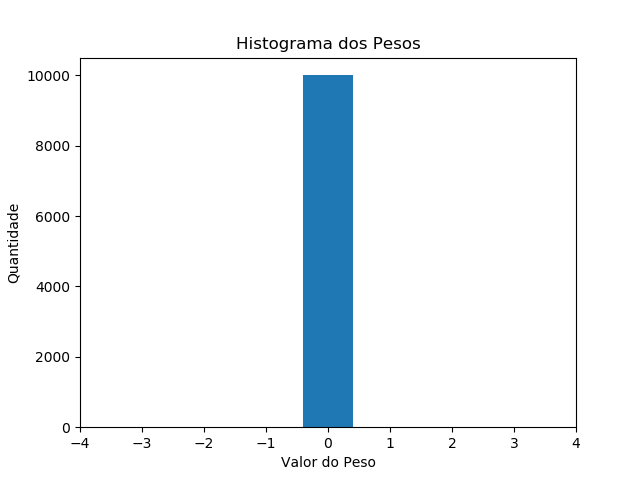
\includegraphics[width=0.5\linewidth]{figures/pesos_zeros}
		\end{figure}
	\end{block}
\end{frame}
%==========================================================================================
\begin{frame}
	\frametitle{Métodos de Inicialização de Pesos}
	\begin{block}{Uns}
		\begin{itemize}
			\item $y \in 1$ 
			\item Inicializa todos o pesos com Uns
			\item Cuidado pois toda a saída será a mesma!! Não utilizar, senão a rede vai se tornar simétrica.
		\end{itemize}
		$	y = np.ones((H, W))$
		\begin{figure}
			\centering
			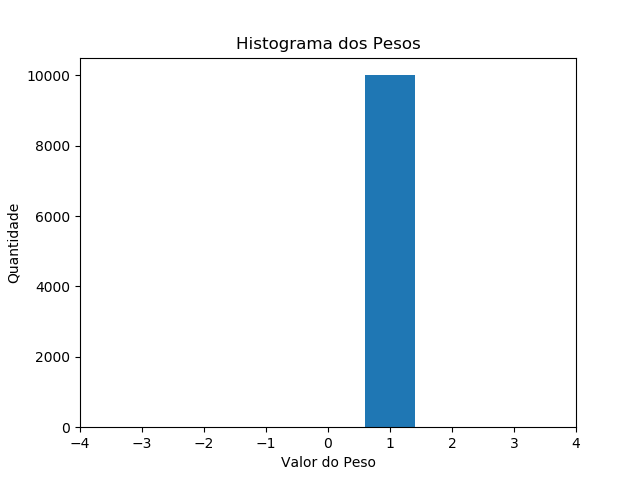
\includegraphics[width=0.5\linewidth]{figures/pesos_ones.png}
		\end{figure}
	\end{block}
\end{frame}
%==========================================================================================
\begin{frame}
	\frametitle{Métodos de Inicialização de Pesos}
	\begin{block}{Distribuição Uniforme Aleatória}
		\begin{itemize}
			\item $y \in [0, 1]$ 
			\item Inicializa todos o pesos com uma Distribuição Uniforme Aleatória 
			\item Quebra a simetria
		\end{itemize}
			$	y = np.random.rand(H, W)$
		\begin{figure}
			\centering
			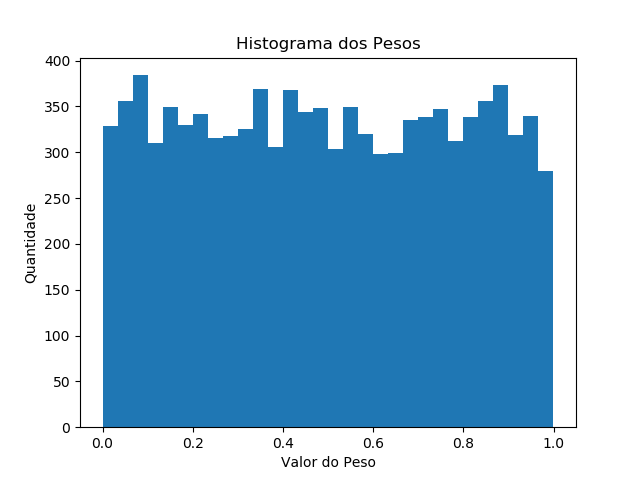
\includegraphics[width=0.5\linewidth]{figures/pesos_uniform.png}
		\end{figure}
	\end{block}
\end{frame}
%==========================================================================================

\begin{frame}
	\frametitle{Métodos de Inicialização de Pesos}
	\begin{block}{Distribuição Normal}
		\begin{itemize}
			\item $y \in [-\infty, +\infty]$ 
			\item Inicializa todos o pesos com uma Distribuição Normal informando média e desvio padrão 
			\item Ajuda a quebrar a simetria da rede
		\end{itemize}
		$	y = np.random.randn(H, W)$
		\begin{figure}
			\centering
			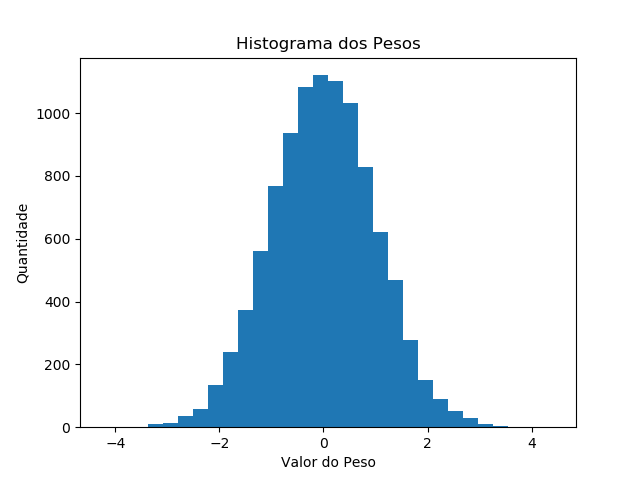
\includegraphics[width=0.5\linewidth]{figures/pesos_normal.png}
		\end{figure}
	\end{block}
\end{frame}
%==========================================================================================
\begin{frame}
	\frametitle{Métodos de Inicialização de Pesos}
	\begin{block}{Glorot Uniforme}
		\begin{columns}
			\begin{column}{0.6 \textwidth}
				\begin{itemize}
					\item $y \in [-\sigma, +\sigma]$
					\item Conhecida como \textbf{Xavier Uniforme}
					\item Leva em consideração o tamanho das camadas
					\item Ajuda a quebrar a simetria
				\end{itemize}
				$	y = 2 * \sigma * np.random.rand(H, W) - \sigma$ \\
				Sendo:
				$\sigma = \sqrt{\frac{6}{in + out}}$ \\
				$in$ é a quantidade de neurônio da camada anterior e $out$ a quantidade de neurônio da camada atual
			\end{column}
		\begin{column}{0.4 \textwidth}
			\begin{itemize}
				\item Torna a convergência mais rápida e eficiente
				\item Uma das melhores inicializações de peso
			\end{itemize}
			\begin{figure}
				\centering
				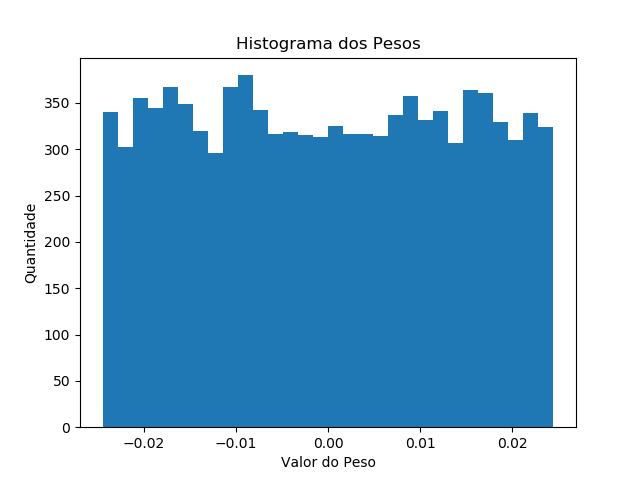
\includegraphics[width=1\linewidth]{figures/pesos_glorot_uniform.png}
			\end{figure}
		\end{column}
		\end{columns}
	\end{block}
\end{frame}
%==========================================================================================
\begin{frame}
	\frametitle{Métodos de Inicialização de Pesos}
	\begin{block}{Glorot Normal}
		\begin{columns}
			\begin{column}{0.6 \textwidth}
				\begin{itemize}
					\item $y \in [-\sigma, +\sigma]$
					\item Conhecida como \textbf{Xavier Normal}
					\item Leva em consideração o tamanho das camadas
					\item Ajuda a quebrar a simetria
				\end{itemize}
				$	y =  \sigma * np.random.randn(H, W) - \sigma$ \\
				Sendo:
				$\sigma = \sqrt{\frac{2}{in + out}}$ \\
				$in$ é a quantidade de neurônio da camada anterior e $out$ a quantidade de neurônio da camada atual
			\end{column}
			\begin{column}{0.4 \textwidth}
				\begin{itemize}
					\item Torna a convergência mais rápida e eficiente
					\item Uma das melhores inicializações de peso
				\end{itemize}
				\begin{figure}
					\centering
					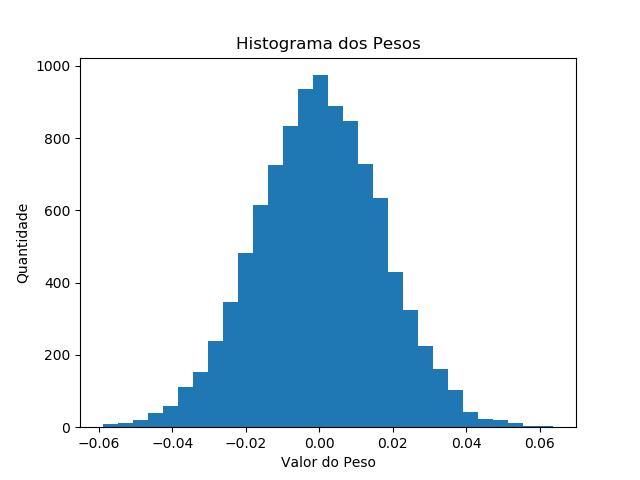
\includegraphics[width=1\linewidth]{figures/pesos_glorot_normal.png}
				\end{figure}
			\end{column}
		\end{columns}
	\end{block}
\end{frame}
%==========================================================================================
\begin{frame}
	\frametitle{Métodos de Inicialização de Pesos}
	\begin{block}{Qual método de inicialização utilizar?}
	\begin{figure}
		\centering
		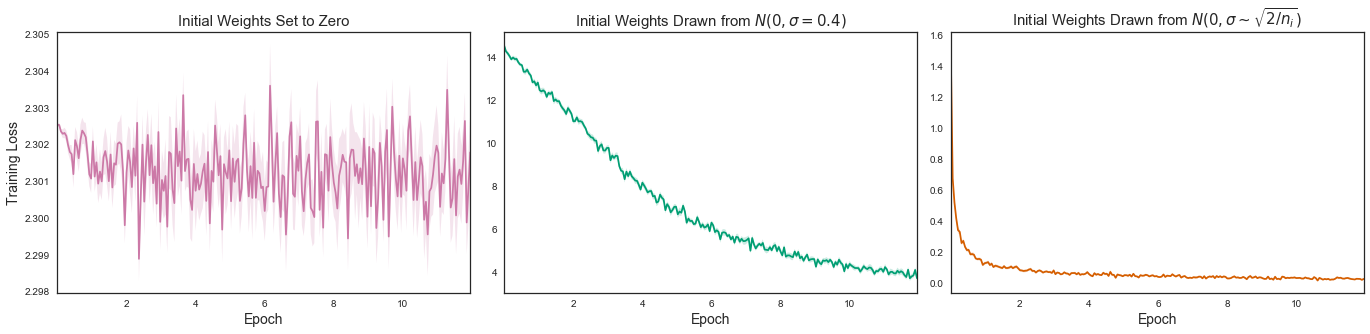
\includegraphics[width=1\linewidth]{figures/weights_init}
	\end{figure}
	Vamos ver isso na prática utilizando o notebook das Redes Neurais! \\
	Vamos refazer nossos experimentos e analisar os resultados
	\end{block}
\end{frame}
%==========================================================================================
\begin{frame}
	\frametitle{Métodos de Inicialização de Pesos}
	\begin{block}{Qual método de inicialização utilizar?}
		\begin{figure}
			\centering
			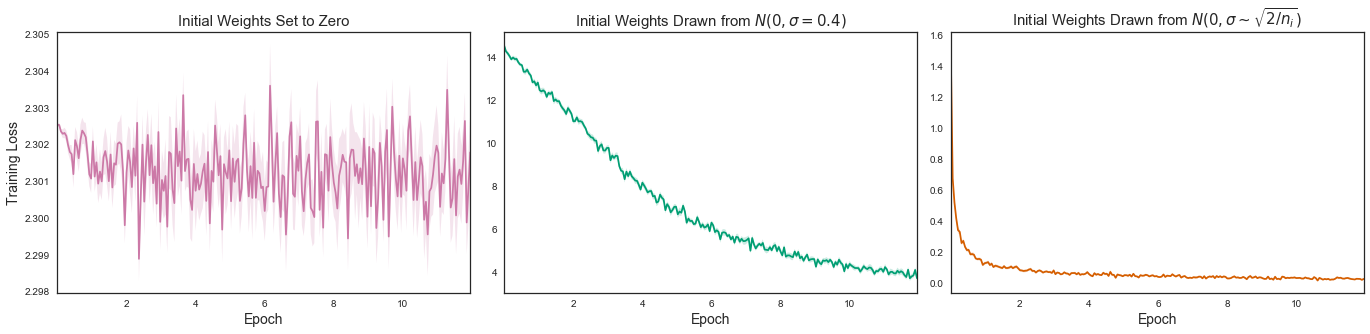
\includegraphics[width=1\linewidth]{figures/weights_init}
		\end{figure}
	\end{block}
\end{frame}
%==========================================================================================
\begin{frame}
	\frametitle{Técnicas de Regularização}
	\begin{block}{Dropout}
		\begin{itemize}
			\item Zerar aleatoriamente a ativação de alguns neurônios por camada utilizando uma probabilidade $p$
			\item Se $p=0.5$ é a probabilidade de zerar 50\% dos neurônios
			\item Cuidado para não tornar a rede ineficiente
			\item A cada iteração diferentes neurônios serão desabilitados, dando a ideia do treinamento de varias sub-redes
			\item os neurônios subsequentes não recebem dados de todos neurônios anteriores.
			\item Uma das melhores técnicas de regularização
			\item Só aplicado no banco de treinamento
			\item Só usado quando ocorre overfitting
		\end{itemize}
	\end{block}
\end{frame}
%==========================================================================================
\begin{frame}
	\frametitle{Técnicas de Regularização}
	\begin{block}{Dropout}
		\begin{figure}
			\centering
			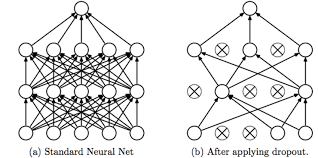
\includegraphics[width=1\linewidth]{figures/dropout}
		\end{figure}
	\end{block}
\end{frame}
%==========================================================================================
\begin{frame}
	\frametitle{Técnicas de Regularização}
	\begin{block}{Regularização L1}
		\begin{itemize}
			\item Criar uma rede menor capaz de resolver o problema
			\item Solução esparsas, atualizando alguns pesos e bias para zeros
			\item Semelhante ao Dropout
			\item Ela deixa apenas os atributos mais relevantes para a rede
			\item A rede é obrigada a aprender com pesos pequenos! E ter o mesmo resultado
			\item A dificuldade é estimar o $\lambda$
			\item Só usado quando ocorre overfitting
		\end{itemize}
	$$J = L(y, w, b) + \frac{\lambda}{m} \sum ||w||$$
	$L(y, w, b)$ é nossa Cost Function \\
	Na L1 é adicionado o termo $ \frac{\lambda}{m} \sum ||w||$  somar o valor absoluto dos pesos e multiplicar por um fator de regularização $\lambda$ e dividir pela Qtd. de amostras. Adicionado isso á nossa MSE, MAE,...
	\end{block}
\end{frame}
%==========================================================================================
\begin{frame}
	\frametitle{Técnicas de Regularização}
	\begin{block}{Regularização L1}
		A derivada da regularização... \\
		Vamos tomar como exemplo a MSE
		$$J = \frac{1}{2} \sum (y - \hat{y})^2 + \frac{\lambda}{m} \sum |w|$$
		A derivada da MSE é:
		$\frac{\partial J1}{\partial w} = -(y - \hat{y})x$ \\
		A derivada do termo pode ser dado por:
		$$\frac{\partial J2}{\partial w} =  \left\{\begin{matrix}
			+1, w > 0
			\\ 
			-1, w < 0
		\end{matrix}\right.$$
	Vamos aplicar isso na formula de atualização dos pesos:
	$w = w - \eta \frac{\partial J}{\partial w}$ Valor inicial - LR * derivada dos pesos 
	\end{block}
\end{frame}
%==========================================================================================

\begin{frame}
	\frametitle{Técnicas de Regularização}
	\begin{block}{Regularização L1}
		Vamos aplicar isso na formula de atualização dos pesos:
		$w = w - \eta \frac{\partial J}{\partial w}$ Valor inicial - LR * derivada dos pesos \\
		Agora... Já que a derivada da soma é a soma das derivadas \\
		$w = w - \eta [\frac{\partial J1}{\partial w} + \frac{\partial J2}{\partial w}]$ \\
		Agora vamos atualizar os pesos da seguinte forma:
		$$w =  \left\{\begin{matrix}
			w - \eta [-(y-\hat{y})x + \frac{\lambda}{m}], w > 0
			\\ 
			w - \eta [-(y-\hat{y})x - \frac{\lambda}{m}], w < 0
		\end{matrix}\right.$$
	\end{block}
\end{frame}
%==========================================================================================

\begin{frame}
	\frametitle{Técnicas de Regularização}
	\begin{block}{Regularização L2}
		\begin{itemize}
			\item Criar uma rede na qual nenhum atributo seja tão mais importante que os outros
			\item Diminui e espalha os valores dos pesos
			\item Mais utilizada que a L1
			\item Conhecida como Weight decay
			\item A dificuldade é estimar o $\lambda$
			\item Só usado quando ocorre overfitting
		\end{itemize}
		$$J = L(y, w, b) + \frac{\lambda}{2m} \sum w_i^2$$
	\end{block}
\end{frame}
%==========================================================================================
\begin{frame}
	\frametitle{Técnicas de Regularização}
	\begin{block}{Regularização L2}
		A derivada da regularização... \\
		Vamos tomar como exemplo a MSE
		$$J = \frac{1}{2} \sum (y - \hat{y})^2 + \frac{\lambda}{2m} \sum w_i^2$$
		A derivada da MSE é:
		$\frac{\partial J1}{\partial w} = -(y - \hat{y})x$ \\
		A derivada do termo pode ser dado por:
		$$\frac{\partial J2}{\partial w} =  \frac{\lambda w}{m}$$
		Vamos aplicar isso na formula de atualização dos pesos:
		$w = w - \eta \frac{\partial J}{\partial w}$ Valor inicial - LR * derivada dos pesos 
	\end{block}
\end{frame}
%==========================================================================================
\begin{frame}
	\frametitle{Técnicas de Regularização}
	\begin{block}{Regularização L2}
		Vamos aplicar isso na formula de atualização dos pesos:
		$w = w - \eta \frac{\partial J}{\partial w}$ Valor inicial - LR * derivada dos pesos \\
		Agora... Já que a derivada da soma é a soma das derivadas \\
		$w = w - \eta [\frac{\partial J1}{\partial w} + \frac{\partial J2}{\partial w}]$ \\
		Agora vamos atualizar os pesos da seguinte forma:
		$$w =  w - \eta [-(y-\hat{y})x + \frac{\lambda w}{m}]$$
	\end{block}
\end{frame}
%==========================================================================================
\begin{frame}
	\frametitle{Técnicas de Regularização}
	\begin{block}{Regularização L2}
		Vamos ver o impacto da regularização nestas imagens
		\begin{figure}
			\centering
			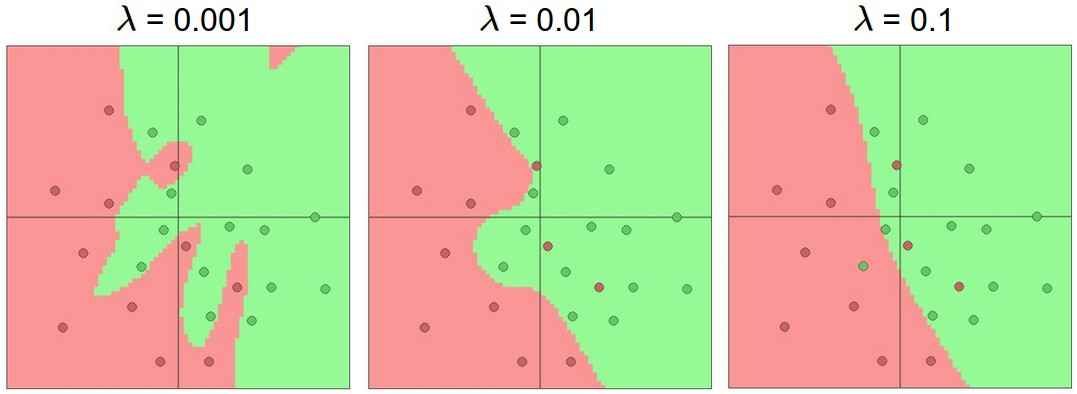
\includegraphics[width=1\linewidth]{figures/comparacao_regularizacao}
		\end{figure}
	Vamos implementar no notebook de redes neurais os métodos de regularização vistos
	\end{block}

\end{frame}
%==========================================================================================
\begin{frame}
	\frametitle{Técnica Momentum}
	\begin{block}{Momentum}
		\begin{itemize}
			\item Utilizada no gradiente descendente
			\item Adiciona velocidade ao Gradiente Descendente
			\item Soma o gradiente da iteração anterior $t-1$ multiplicado por um fator momentum $\mu$
			\item 	\href{https://github.com/mafaldasalomao/pavic_treinamento_ml/blob/main/Machine_Learning/figures/nomomentum1d.gif?raw=true}{\beamergotobutton{Sem Momentum}}
			\item \href{https://github.com/mafaldasalomao/pavic_treinamento_ml/blob/main/Machine_Learning/figures/momentum1d.gif?raw=true}{\beamergotobutton{Com Momentum}}
			\item Fonte \href{https://machinelearningcoban.com/2017/01/16/gradientdescent2/}{\beamergotobutton{Fonte}}
			
		\end{itemize}
		
		$$\triangledown w = \eta \frac{\partial J}{\partial w} + \mu \triangledown w^{t-1}$$
		Vamos implementar no notebook de redes neurais o nosso momentum
	\end{block}
\end{frame}
%==========================================================================================


%==========================================================================================
\begin{frame}
	\frametitle{Mini-Batch}
	\begin{block}{Mini-Batch}
		\begin{itemize}
			\item Divide o treinamento em conjuntos menores (memória)
			\item É importante dar shuffle (embaralhar) antes de cada epoch
			\item 1 epoch = processar todos os batchs
			\item Em geral, é a estratégia de GD mais utilizada	
			
		\end{itemize}
		Vamos tomar um dataset com $100$ amostras e seja dividi-lo em $10$ batchs. Cada batch terá $10$ amostras.
		\begin{figure}
			\centering
			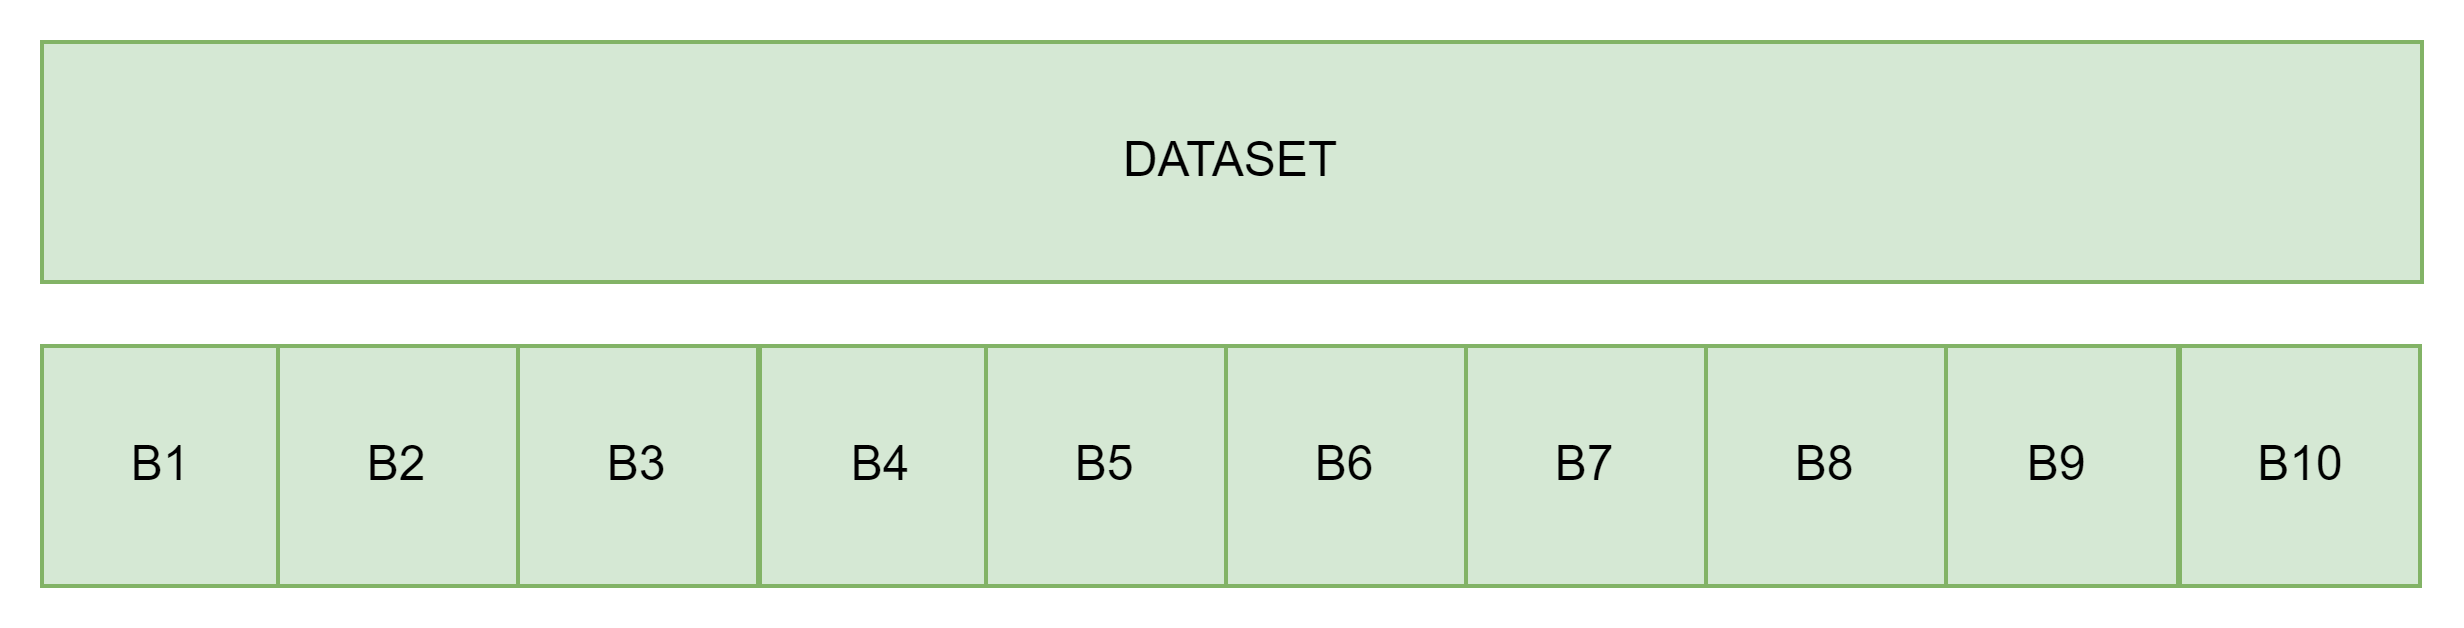
\includegraphics[width=1\linewidth]{figures/minibatch.png}
		\end{figure}
		
	\end{block}
\end{frame}
%==========================================================================================
\begin{frame}
	\frametitle{Gradiente Descendente}
	\begin{block}{Gradiente Descendente}
		Qual a diferença entre o Gradiente Estocástico para o Gradiente Baseado em Mini-batch e Bath \\
		\begin{columns}
			\begin{column}{0.3 \textwidth}
				\textbf{Stochastic Gradient} \\
				Amostra por amostra\\
				Aponta para a direção da amostra \\
				Converge lentamente \\
				Anula vetorização
			\end{column}
			\begin{column}{0.3 \textwidth}
				\textbf{Mini-Batch GD} \\
				Calcula as atualizações por lote \\
				Aponta para a direção que desce \\
				Converge rápido \\
				Rápida execução
			\end{column}
			\begin{column}{0.3 \textwidth}
				\textbf{Batch GD} \\
				Todas as amostras de uma vez \\
				Aponta para a direção que desce sempre \\
				Converge rápido \\
				Lenta execução
			\end{column}
		\end{columns}
		
	\end{block}
\end{frame}

	
%==========================================================================================
\begin{frame}
	\frametitle{Learning Rate Decay}
	\begin{block}{Learning Rate Decay}
		\begin{itemize}
			\item A learning rate alta irá dificultar o aprendizado do algoritmo, mas se livrará de mínimos locais
			\item A learning rate baixa irá ajudar no aprendizado da rede mas irá ter problemas com mínimos locais
			\item Com a Learning Rate Decay, a taxa de aprendizado será reduzida ao longo das épocas
		\end{itemize}
	\end{block}
\end{frame}	
	%==========================================================================================
	\begin{frame}
		\frametitle{Learning Rate Decay}
		\begin{block}{Learning Rate Decay - Time-based}
			$$\lambda_t = \frac{1}{1 + \alpha *t}$$ 
			Onde $t$ são as épocas
			\begin{columns}
				\begin{column}{0.3 \textwidth}
					\begin{figure}
						\centering
						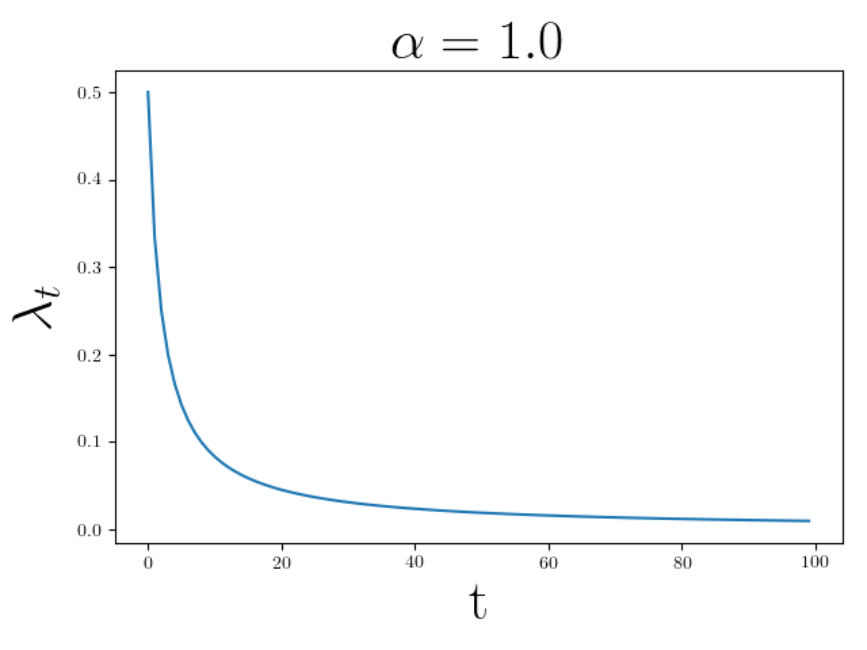
\includegraphics[width=1\linewidth]{figures/lr_decay1.png}
					\end{figure}
				\end{column}
				\begin{column}{0.3 \textwidth}
					\begin{figure}
						\centering
						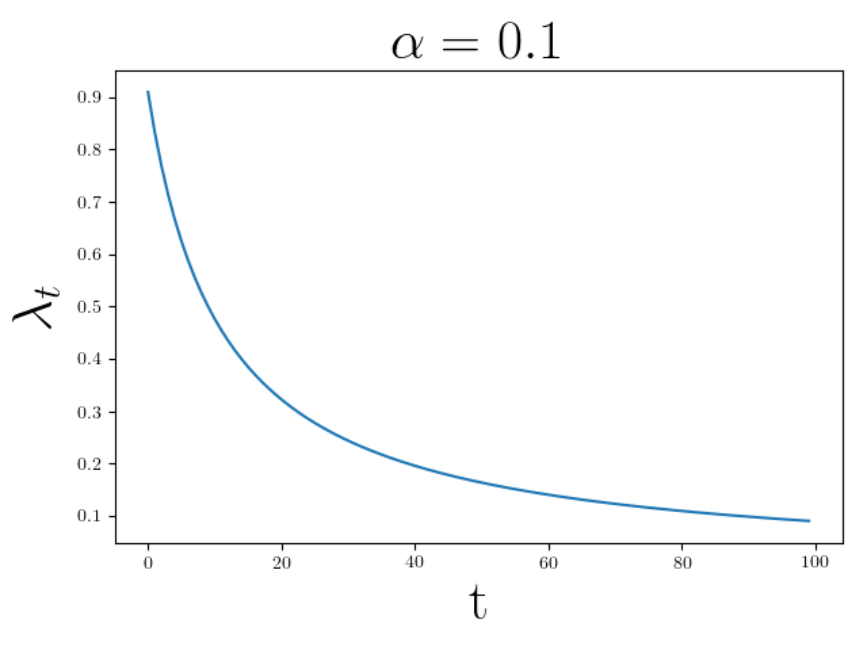
\includegraphics[width=1\linewidth]{figures/lr_decay2.png}
					\end{figure}
				\end{column}
				\begin{column}{0.3 \textwidth}
					\begin{figure}
						\centering
						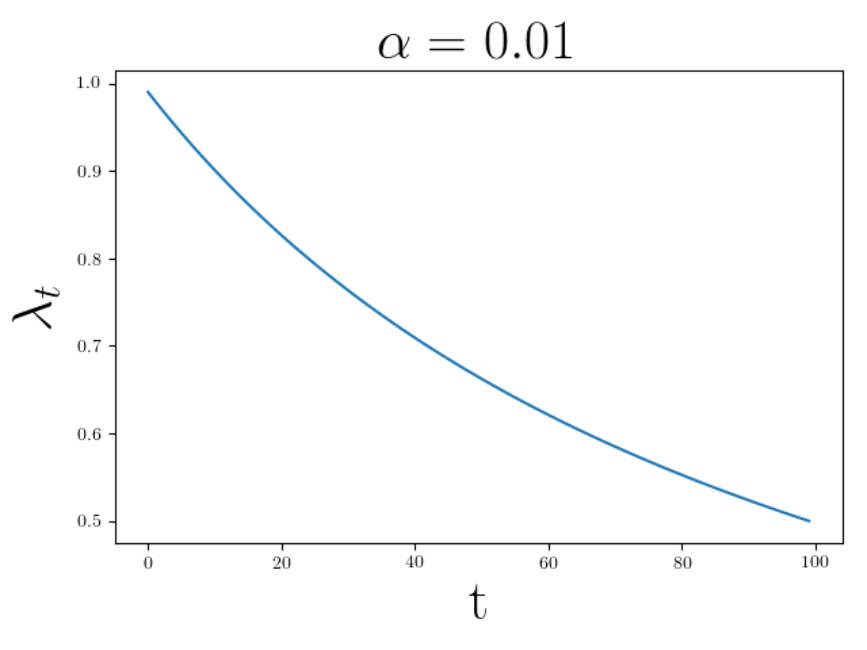
\includegraphics[width=1\linewidth]{figures/lr_decay3.png}
					\end{figure}
				\end{column}
			\end{columns}
		\end{block}
	\end{frame}	

%==========================================================================================
\begin{frame}
	\frametitle{Learning Rate Decay}
	\begin{block}{Learning Rate Decay - Exponential}
		$$\lambda_t = \lambda_0 *\alpha^t$$ 
		Onde $\alpha^t$ é o fator exponencial do decaimento da Learning rate
		\begin{columns}
			\begin{column}{0.3 \textwidth}
				\begin{figure}
					\centering
					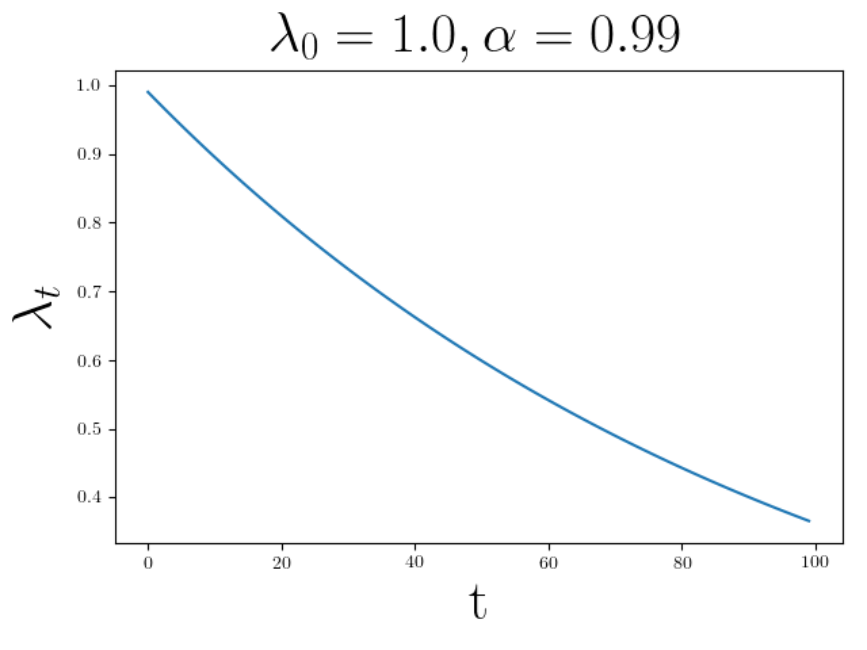
\includegraphics[width=1\linewidth]{figures/lr_decay4.png}
				\end{figure}
			\end{column}
			\begin{column}{0.3 \textwidth}
				\begin{figure}
					\centering
					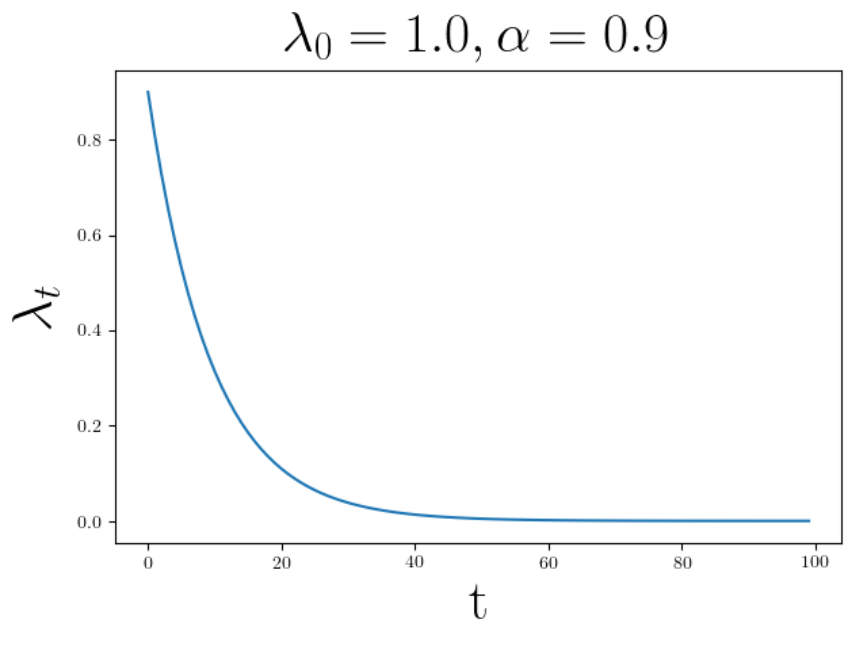
\includegraphics[width=1\linewidth]{figures/lr_decay5.png}
				\end{figure}
			\end{column}
			\begin{column}{0.3 \textwidth}
				\begin{figure}
					\centering
					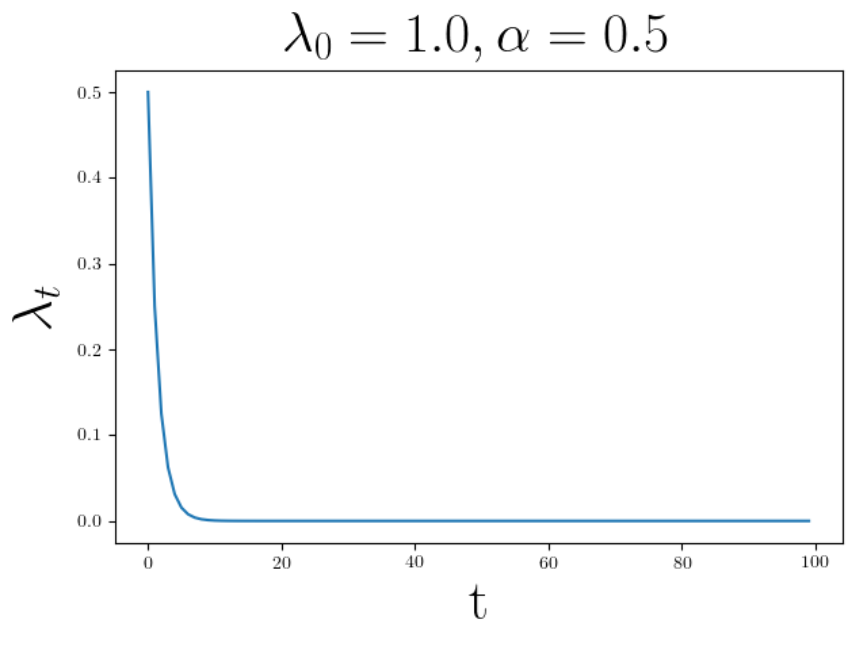
\includegraphics[width=1\linewidth]{figures/lr_decay6.png}
				\end{figure}
			\end{column}
		\end{columns}
	\end{block}
\end{frame}	
%==========================================================================================
\begin{frame}
		\frametitle{Learning Rate Decay}
		\begin{block}{Learning Rate Decay - Staircase}
			$$\lambda_t = \lambda_0 *\alpha^{t/ds}$$ 
			Onde $\alpha^{t/ds}$ é o fator exponencial do decaimento da Learning rate e o $ds$ é de quanta em quanta épocas ocorrerá o decay.
			\begin{columns}
				\begin{column}{0.3 \textwidth}
					\begin{figure}
						\centering
						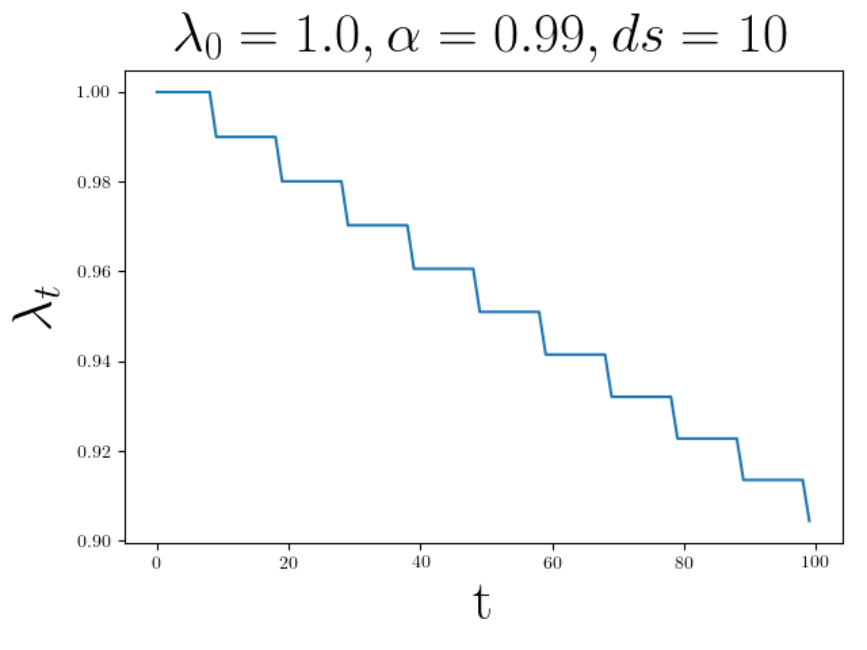
\includegraphics[width=1\linewidth]{figures/lr_decay7.png}
					\end{figure}
				\end{column}
				\begin{column}{0.3 \textwidth}
					\begin{figure}
						\centering
						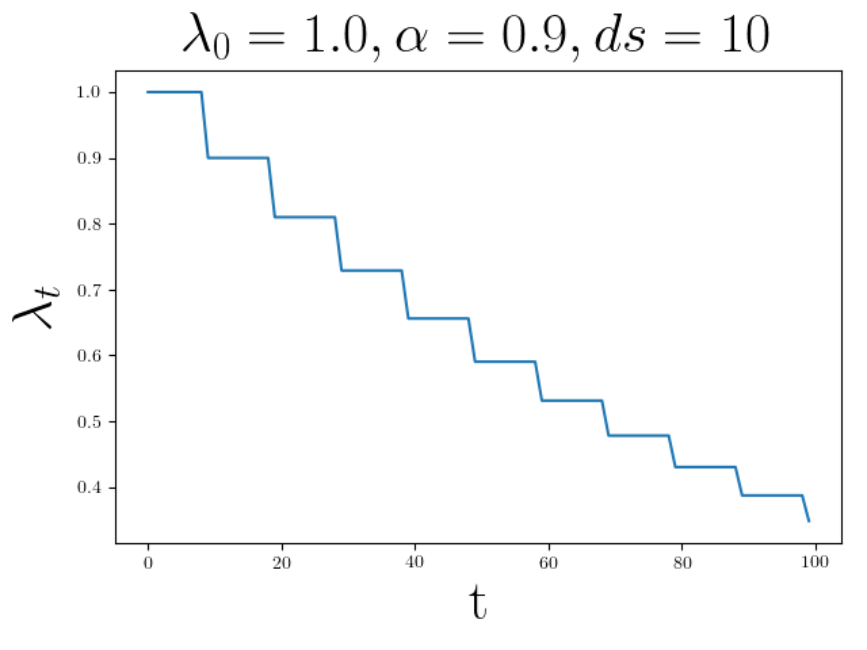
\includegraphics[width=1\linewidth]{figures/lr_decay8.png}
					\end{figure}
				\end{column}
				\begin{column}{0.3 \textwidth}
					\begin{figure}
						\centering
						\includegraphics[width=1\linewidth]{figures/lr_decay9.png}
					\end{figure}
				\end{column}
			\end{columns}
		\end{block}
	\end{frame}	
	
%==========================================================================================
\begin{frame}
	\frametitle{Stop Early}
	\begin{block}{Stop Early}
		\begin{itemize}
			\item A ideia é guardar seu melhor modelo. Quando a perda tiver valor mínimo em validação!
			\item Fator patient indica quando o modelo deve parar de treinar a partir da última melhor acurácia. Por exemplo, se na época 7 o modelo apresentou acurácia de 75\% e nas 10 (patient) próximas épocas o modelo não melhorou, então o treinamento é finalizado.
		\end{itemize}
		\begin{figure}
			\centering
			\includegraphics[width=0.35\linewidth]{figures/early_stop}
		\end{figure}
	\end{block}
\end{frame}	
	
%==========================================================================================
\begin{frame}
	\frametitle{Batch Normalization}
	\begin{block}{Batch Normalization}
		\begin{itemize}
			\item Normaliza entradas ou saídas das camadas de ativação
			\item Estima a média e desvio padrão baseado no batch (média móvel)
			\item Regulariza camadas e não neurônios
			\item Pode substituir o dropout
			\item Uma das melhores técnicas
			\item Não usado na validação ou teste!
		\end{itemize}
	\end{block}
\end{frame}	

%==========================================================================================
\begin{frame}
	\frametitle{Batch Normalization}
	\begin{block}{Batch Normalization - FeedForward}
	\begin{columns}
		\begin{column}{0.5 \textwidth}
			\begin{figure}
				\centering
				\includegraphics[width=1\linewidth]{figures/batch_norm_feed.png}
			\end{figure}
		\end{column}
		\begin{column}{0.5 \textwidth}
			\begin{itemize}
				\item Cada batch será normalizado subtraindo da média $\mu$ e dividindo pelo desvio padrão $\sigma^2$ = $\hat{x}_i$
				\item $\gamma$ e $\beta$ são parâmetros que a rede vai aprender
				\item se $\gamma = \sigma^2 $ e $\mu = \beta$ a função se anula, assim a rede pode recusar o batch normalization sozinha!
			\end{itemize}
		\end{column}
	\end{columns}

	\end{block}
\end{frame}	
	
%==========================================================================================
\begin{frame}
	\frametitle{Batch Normalization}
	\begin{block}{Batch Normalization - Backpropagation}
		\begin{figure}
			\centering
			\includegraphics[width=1\linewidth]{figures/batch_norm_back.png}
		\end{figure}
	\end{block}
\end{frame}		
	
%==========================================================================================
\begin{frame}
	\frametitle{Freezing}
	\begin{block}{Freezing}
		\begin{itemize}
			\item Congelamento de certas camadas no \textbf{treinamento}
			\item Muito usada em transfer learning e Fine-tuning
		\end{itemize}
		\begin{figure}
			\centering
			\includegraphics[width=0.7\linewidth]{figures/simple_nn.png}
		\end{figure}
	\end{block}
\end{frame}			
	
	
	
	
\begin{frame}	
\frametitle{Highlighting text}
%
%\begin{align}
%	a + b  q q= c \\        
%	a = c - b
%\end{align}
In this slide, some important text will be
\alert{highlighted} because it's important.
Please, don't abuse it.

\begin{block}{Remark}
Sample text
\end{block}

\begin{alertblock}{Important theorem}
Sample text in red box
\end{alertblock}

\begin{examples}
Sample text in green box. The title of the block is ``Examples".
\end{examples}
\end{frame}

\end{document}